\documentclass[12pt,twoside]{report}

% some definitions for the title page
\newcommand{\reporttitle}{A Virtual Volumetric Screen}
\newcommand{\reportauthor}{Robert Buxton}
\newcommand{\supervisor}{Dr Nicole Salomons}
\newcommand{\reporttype}{MEng Individual Project}
\newcommand{\degreetype}{Computing MEng}  

% load some definitions and default packages
%%%%%%%%%%%%%%%%%%%%%%%%%%%%%%%%%%%%%%%%%
% University Assignment Title Page 
% LaTeX Template
% Version 1.0 (27/12/12)
%
% This template has been downloaded from:
% http://www.LaTeXTemplates.com
%
% Original author:
% WikiBooks (http://en.wikibooks.org/wiki/LaTeX/Title_Creation)
%
% License:
% CC BY-NC-SA 3.0 (http://creativecommons.org/licenses/by-nc-sa/3.0/)
% 
%
%%%%%%%%%%%%%%%%%%%%%%%%%%%%%%%%%%%%%%%%%
%----------------------------------------------------------------------------------------
%	PACKAGES AND OTHER DOCUMENT CONFIGURATIONS
%----------------------------------------------------------------------------------------
\usepackage[usenames,dvipsnames]{xcolor}
\usepackage[a4paper,hmargin=2.0cm,vmargin=2.0cm,includeheadfoot]{geometry}
\usepackage{textpos}
\usepackage[style=numeric, backend=biber]{biblatex} % for bibliography
\usepackage{csquotes}
\usepackage{tabularx,longtable,multirow,subfigure,caption}%hangcaption
\usepackage{fancyhdr} % page layout
\usepackage{url} % URLs
\usepackage[english]{babel}
\usepackage{amsmath}
\usepackage{graphicx}
\usepackage{svg}
\usepackage[many,minted]{tcolorbox}
\usepackage{epstopdf} % automatically replace .eps with .pdf in graphics
\usepackage{array}
\usepackage{latexsym}
\usepackage[pdftex,hypertexnames=false,colorlinks]{hyperref} % provide links in pdf
\usepackage{opensans}
\usepackage{float}
\usepackage{adjustbox}
\usepackage{listings}
\usepackage{fontspec}
\usepackage[all]{hypcap}
\usepackage{enumitem}

\addbibresource{references.bib}

\hypersetup{pdftitle={},
  pdfsubject={},
  pdfauthor={},
  pdfkeywords={},
  pdfstartview=FitH,
  pdfpagemode={UseOutlines},% None, FullScreen, UseOutlines
  bookmarksnumbered=true, bookmarksopen=true, colorlinks,
  citecolor=black,%
  filecolor=black,%
  linkcolor=black,%
  urlcolor=black}


% Removes annoying errors
\hbadness=99999 


\setmainfont{XCharter}
\setmonofont{CMU Typewriter Text}
%%% Default fonts
% \renewcommand*{\rmdefault}{bch}
% \renewcommand*{\ttdefault}{cmtt}

%%% Default settings (page layout)
\setlength{\parindent}{0em}  % indentation of paragraph

\setlength{\parindent}{0em}  % indentation of paragraph

\setlength{\headheight}{14.5pt}
\pagestyle{fancy}
\renewcommand{\chaptermark}[1]{\markboth{\chaptername\ \thechapter.\ #1}{}}
%\fancyhead[RO]{\sffamily \textbf{\thepage}} %Page no.in the right on even pages
%\fancyhead[LE]{\sffamily \textbf{\thepage}} %Page no. in the left on odd pages

\fancyfoot[ER,OL]{\thepage}%Page no. in the left on
%odd pages and on right on even pages
\fancyfoot[OC,EC]{\sffamily }
\renewcommand{\headrulewidth}{0.1pt}
\renewcommand{\footrulewidth}{0.1pt}
\captionsetup{margin=10pt,font=small,labelfont=bf}


%--- chapter heading

\def\@makechapterhead#1{%
  \vspace*{10\p@}%
  {\parindent \z@ \raggedright \sffamily
    \interlinepenalty\@M
    \Huge\bfseries \thechapter \space\space #1\par\nobreak
    \vskip 30\p@
  }}

%--- chapter heading

\def\@makechapterhead#1{%
  \vspace*{10\p@}%
  {\parindent \z@ \raggedright \sffamily
    %{\Large \MakeUppercase{\@chapapp} \space \thechapter}
    %\\
    %\hrulefill
    %\par\nobreak
    %\vskip 10\p@
    \interlinepenalty\@M
    \Huge\bfseries \thechapter \space\space #1\par\nobreak
    \vskip 30\p@
  }}

%---chapter heading for \chapter*  
\def\@makeschapterhead#1{%
  \vspace*{10\p@}%
  {\parindent \z@ \raggedright
    \sffamily
    \interlinepenalty\@M
    \Huge \bfseries  #1\par\nobreak
    \vskip 30\p@
  }}
\allowdisplaybreaks

% load some macros
% Here, you can define your own macros. Some examples are given below.

% \newcommand{\R}[0]{\mathds{R}} % real numbers
% \newcommand{\Z}[0]{\mathds{Z}} % integers
% \newcommand{\N}[0]{\mathds{N}} % natural numbers
% \newcommand{\C}[0]{\mathds{C}} % complex numbers
% \renewcommand{\vec}[1]{{\boldsymbol{{#1}}}} % vector
% \newcommand{\mat}[1]{{\boldsymbol{{#1}}}} % matrix

\newcommand{\tocite}{{\color{red} \small ToCite }} % placeholder for later citation
\newcommand{\todo}{{\color{red} \small TODO }} % placeholder for later citation

\lstdefinestyle{tree}{
literate=
  {├}{{\smash{\raisebox{-1ex}{\rule{1pt}{\baselineskip}}}\raisebox{0.5ex}{\rule{1ex}{1pt}}}}1
{─}{{\raisebox{0.5ex}{\rule{1.5ex}{1pt}}}}1
{└}{{\smash{\raisebox{0.5ex}{\rule{1pt}{\dimexpr\baselineskip-1.5ex}}}\raisebox{0.5ex}{\rule{1ex}{1pt}}}}1
}

\newcommand{\nixstore}[2][1]{\textcolor{Purple}{\texttt{/nix/store/}}\textcolor{RoyalBlue}{\texttt{#1}-}\textcolor{Orange}{\texttt{#2}}}

\newcommand{\mynewminted}[3]{%
  \newminted[#1]{#2}{#3}%
  \tcbset{myminted/#1/.style={minted language=#2,minted options={#3}}}}


%Programming Languages
\mynewminted{nix}{nix}{
  breaklines,
  linenos,
  autogobble,
  numbersep=2mm,
  fontsize=\footnotesize,
  frame=none}

\mynewminted{cpp}{cpp}{
  breaklines,
  linenos,
  autogobble,
  numbersep=2mm,
  fontsize=\footnotesize,
  frame=none}

\mynewminted{shell}{shell}{
  breaklines,
  autogobble,
  fontsize=\footnotesize,
  frame=none}


\newtcbinputlisting[auto counter,number within=section,list inside=mypyg]{\codeBoxFile}[4][]{%
  center,
  listing engine=minted,
  listing only,
  title={{\color{Black} \textbf{Listing \thetcbcounter:}} {\small #4}},
  % list entry={\protect\numberline{\thetcbcounter}#3},
  listing file={#3},
  enhanced jigsaw,
  breakable,
  colframe = Apricot!25,
  colback  = Apricot!10,
  coltitle = Apricot!20!black,
  drop fuzzy shadow,
  before skip = 20pt,
  after skip = 20pt,
  myminted/#2,
  #1}

%Boxes
\newtcolorbox[auto counter,number within=section]{figureBox}[2][]
{
  center,
  enhanced jigsaw,
  breakable,
  colframe = Apricot!25,
  colback  = Apricot!10,
  coltitle = Apricot!20!black,
  drop fuzzy shadow,
  title    = {{\color{Black} \textbf{Figure \thetcbcounter:}} {\small #2}},
  before skip = 20pt,
  after skip = 20pt,
  before upper={\centering \color{Gray!20!black}},
  #1,
}

\newtcbox[auto counter,number within=section]{\pictureBox}[2][]
{
  enhanced jigsaw,
  nobeforeafter,
  colframe = Apricot!25,
  colback= Apricot!25,
  coltitle = Apricot!20!black,
  drop fuzzy shadow,
  boxsep=3pt,
  left=0pt,
  right=0pt,
  top=0pt,
  bottom=0pt,
  title    = {{\color{Black} \textbf{Figure \thetcbcounter:}} {\small #2}},
  #1,
}

%Invisible box

\newtcolorbox{invisBox}{
  center,
  enhanced jigsaw,
  breakable,
  before skip=20pt,
  after skip=20pt,
  left=0pt,
  right=0pt,
  top=0pt,
  bottom=0pt,
  colframe=white, % Frame color
  colback=white,  % Background color
  opacityframe=0, % Frame opacity
  opacityback=0   % Background opacity
}

% load title page
\begin{document}
% !TEX root = ./main.tex

% Last modification: 2015-08-17 (Marc Deisenroth)
\begin{titlepage}

\newcommand{\HRule}{\rule{\linewidth}{0.5mm}} % Defines a new command for the horizontal lines, change thickness here

%----------------------------------------------------------------------------------------
%	LOGO SECTION
%----------------------------------------------------------------------------------------


\includegraphics[width = 4cm]{./figures/imperial}\\[0.5cm] 

\center % Center everything on the page
 
%----------------------------------------------------------------------------------------
%	HEADING SECTIONS
%----------------------------------------------------------------------------------------

\textsc{\LARGE \reporttype}\\[1.5cm] 
\textsc{\Large Department of Computing}\\[0.5cm] 
\textsc{\large Imperial College of Science, Technology and Medicine}\\[0.5cm] 

%----------------------------------------------------------------------------------------
%	TITLE SECTION
%----------------------------------------------------------------------------------------

\HRule \\[0.4cm]
{ \huge \bfseries \reporttitle}\\ % Title of your document
\HRule \\[1.5cm]
 
%----------------------------------------------------------------------------------------
%	AUTHOR SECTION
%----------------------------------------------------------------------------------------

\begin{minipage}{0.4\textwidth}
\begin{flushleft} \large
\emph{Author:}\\
\reportauthor % Your name
\end{flushleft}
\end{minipage}
~
\begin{minipage}{0.4\textwidth}
\begin{flushright} \large
\emph{Supervisor:} \\
\supervisor % Supervisor's Name
\end{flushright}
\end{minipage}\\[4cm]




%----------------------------------------------------------------------------------------


%----------------------------------------------------------------------------------------
%	DATE SECTION
%----------------------------------------------------------------------------------------

{\large \today} % Date, change the \today to a set date if you want to be precise


\vfill % Fill the rest of the page with whitespace
Submitted in partial fulfillment of the requirements for the \degreetype~of Imperial College London

\end{titlepage}



% page numbering etc.
\pagenumbering{roman}
\clearpage{\pagestyle{empty}\cleardoublepage}
\setcounter{page}{1}
\pagestyle{fancy}

% %%%%%%%%%%%%%%%%%%%%%%%%%%%%%%%%%%%%
\begin{abstract}
	This thesis presents the development of a virtual volumetric screen designed to simulate volumetric displays for Human-Computer Interaction (HCI) research. The primary objective is to create a cost-effective, reproducible, and simple system that enables researchers to explore the usability of volumetric displays without requiring access to expensive and specialised hardware. The system employs head and hand tracking to render 3D content on a standard 2D monitor, creating the illusion of depth and allowing natural interaction with virtual objects. \\
	
	A comprehensive user study was conducted to evaluate the effectiveness of the system. The study compared user performance in tasks requiring spatial interaction under different conditions: 3D versus 2D views and direct hand interaction versus teleoperation. The results showed a significant improvement in task performance when using a 3D view with direct hand interaction, highlighting the importance of intuitive and immersive interaction modes in volumetric display research. \\
	
	Future work includes expanding the system's compatibility with different hardware and operating systems, improving hand tracking accuracy, and exploring multi-user support. 
\end{abstract}

% \cleardoublepage
% %%%%%%%%%%%%%%%%%%%%%%%%%%%%%%%%%%%%
\section*{Acknowledgments}
I would like to thank \textbf{in order of importance}:
\begin{itemize}[noitemsep]
	% \item ChatGPT
    \item My supervisor Dr Nicole Salomons for her guidance and support throughout this project so far.
    \item My loving family who still think I am studying physics (\textbf{Mabel}) for some reason.
\end{itemize}
\clearpage{\pagestyle{empty}\clearpage}

%%%%%%%%%%%%%%%%%%%%%%%%%%%%%%%%%%%%
%--- table of contents
\fancyhead[RE,LO]{\sffamily {Table of Contents}}
\tableofcontents


\clearpage{\pagestyle{empty}\clearpage}
\pagenumbering{arabic}
\setcounter{page}{1}
\fancyhead[LE,RO]{\slshape \rightmark}
\fancyhead[LO,RE]{\slshape \leftmark}

%%%%%%%%%%%%%%%%%%%%%%%%%%%%%%%%%%%%
\chapter{Introduction}
\section{Motivations}

Volumetric Displays are a new and exciting technology that has the potential to revolutionize the way we interact with computers. They are a type of 3D display that can be viewed from any angle without the need for special glasses by multiple people simultaneously. \tocite These displays differ from a virtual reality experience in that they are not immersive, but rather they are a window into a virtual world (See Fig~\ref{fig:volumetric-display-examples}). There is a not a consensus what the best way to build a volumetric display is and as I cover in the background section there are many approaches being attempted by research groups both academic and industrial. 

\begin{figureBox}[label={fig:volumetric-display-examples}]{Two different volumetric displays}
    \begin{minipage}[t]{0.48\textwidth}
   
      \small {a) Example one.}
    \end{minipage}\hfill
    \begin{minipage}[t]{0.48\textwidth}

      \small {b) Example two.}
    \end{minipage}
\end{figureBox}

It is difficult to conduct human-computer interaction (HCI) research into volumetric displays because these devices are not widely available, expensive to manufacture, and have high bandwidth requirements. This makes it difficult to conduct user studies and experiments. People have created virtual simulations of volumetric displays to try and solve this problem, \tocite but these solutions are often complicated and difficult and expensive to replicate.

\section{Objectives}

With this paper, we aim to provide a cheap, multi-platform, lightweight and simple platform for simulating volumetric displays. We hope that this will enable researchers to conduct HCI research into volumetric displays without the need for expensive hardware. We aim to make the following contributions:
\subsection{Volumetric Simulator}
We plan to create a platform for simulating volumetric displays that is:
\begin{itemize}
    \item \textbf{Multi-platform}: We package our platform in nix \cite{dolstra2004nix} which allows it to be run on any platform that supports nix  (Linux, macOS, and (Windows through WSL \tocite)) on a large range of nix supported hardware \tocite by running a single line of code \texttt{sudo nix run github:RobbieBuxton/VolumetricSim}.
    
    \item \textbf{Lightweight}: By using simple rending algorithms in OpenGL to render the volumetric display our software is relatively computationally cheap to run compared to typical rendering engines that might be used for HCI research like Unity \tocite. 
    
    \item \textbf{Cheap}: By relying just on a depth camera and a normal monitor our software requires minimal hardware to run. This makes it cheap to run and easy to replicate.
    
    \item \textbf{Simple}: We have designed our software to be as simple as possible by taking advantage of the nix package manager to handle all the dependencies and by depending on simple external libraries like \texttt{dlib} \tocite to handle more complicated tasks like face detection. This makes it easy to replicate and modify.
    
    \item \textbf{Reproducible:} By building with nix we can guarantee that any experiments conducted using the simulator will be completely reproducible.
\end{itemize}

\subsection{User experiment}
We plan to conduct an HCI user study to demonstrate the utility of our volumetric simulation platform. We will conduct a user study to compare the effectiveness of using hand tracking to interact directly with an ethereal/incorporeal volumetric display compared to a via tele-operation with a corporeal/tangible display (See Fig~\ref{fig:user experiment}). 

\begin{figureBox}[label={fig:user experiment}]{User experiment}
    % \includegraphics[width = 0.5\linewidth]{}
\end{figureBox}

%%%%%%%%%%%%%%%%%%%%%%%%%%%%%%%%%%%%
\chapter{Ethical Discussion}
\section{User Study}
We ran a user study to evaluate our simulator titled "A Virtual Volumetric Screen User Study". We undertook Imperial College London's "Science Engineering Technology Research Ethics Committee process" which was reviewed by the "Research Governance and Integrity Team" and the head of the computing department. We gained approval on the 2nd May 2024 and ran our study between May and July \textcolor{red}{find first and last date of participants}. 

\subsection{Human participants}
As we ran our study on human participants we had to ensure we conducted our study in an ethical way. We consulted the Equality Act 2010 to make sure we did not exclude any participants \tocite. We were also careful to not use any participants that might feel perceived pressure to participate or might feel influenced by the researchers conducting the study. Participants were presented with an information sheet and a consent form before the study began.   

\subsection{Data collection}
While collecting data for our study we were careful to comply with the local regulations (\textbf{GDPR}) \tocite. All data was stored on a secure computer on campus and was only accessible by the researchers, or was stored on Imperials secure cloud network. We also made sure to anonymise the data when presenting it in our report. Data will be retained until 30th June 2034.

\section{Volumetric Simulator}
\subsection{Military applications}
This technology in theory could be used for military applications, however, we believe is unlikely to be used for such purposes, and if it was, it would not be directly used in combat and would be no more dangerous than other existing technologies.

\subsection{Copywrite Limitations}
\subsubsection{Open Source}
We will be using the Azure Kinect SDK which is licensed under the MIT license. We will also be using the Nix package manager which is licensed under the LGPL-2.1 license. Furthermore, we will also be using the Nixpkgs repository which is licensed under the MIT license. We will also be using the \texttt{dlib} library which is licensed under the Boost Software License 1.0 (BSL-1.0). We will also be using the OpenGL library which is licensed under the open-source license for the use of sample Implementation (SI). Furthermore, we will also be using the GLFW library which is licensed under the zlib license. We will also be using the GLM library which is licensed under the MIT license. We will also be using the OpenCV license under the Apache License.

\subsubsection{Proprietary}
Furthermore, we use Microsoft's proprietary depth engine designed to work with the Azure Kinect SDK which is not open source.

\textcolor{red}{Add other libraries we use}
\label{sect:ethics}

%%%%%%%%%%%%%%%%%%%%%%%%%%%%%%%%%%%%
\chapter{Background}
\section{Volumetric displays}

Volumetric displays \cite{1492264} provide a three-dimensional viewing experience by emitting light from each voxel, or volume element, in a 3D space. This approach enables the accurate representation of virtual 3D objects while providing accurate focal depth, motion parallax, and vergence. Vergence refers to the rotation of a viewer's eye to fixate on the same point they are focusing on. Moreover, volumetric displays allow multiple users to view the same display from different angles, providing unique perspectives of the same object simultaneously.

\subsection{Swept Volume Displays}
Swept volume displays are one prominent category of volumetric displays. They employ a moving 2D display to create a 3D image through the persistence of vision effects. This is achieved by moving the 2D display through a 3D space at high speeds while emitting light from the display where it reaches the position of each corresponding voxel. Common techniques for achieving this include using a rotating mirror \cite{10.1117/12.480930}, an emitting screen, typically an LED-based \cite{Gately:11}, or a transparent projector screen \cite{keane_volumetric_2016}. There currently exist commercial products that implement this technique as can be seen in Fig~\ref{fig:voxon} and Fig~\ref{fig:brightbox}.

\begin{invisBox}
  
  \pictureBox[label={fig:voxon}]{The VXR4612 3D Volumetric Display, a projector-based persistence of vision display produced by Voxon Photonics. \cite{voxon2}}{
    \adjustbox{height=4cm, keepaspectratio}{
      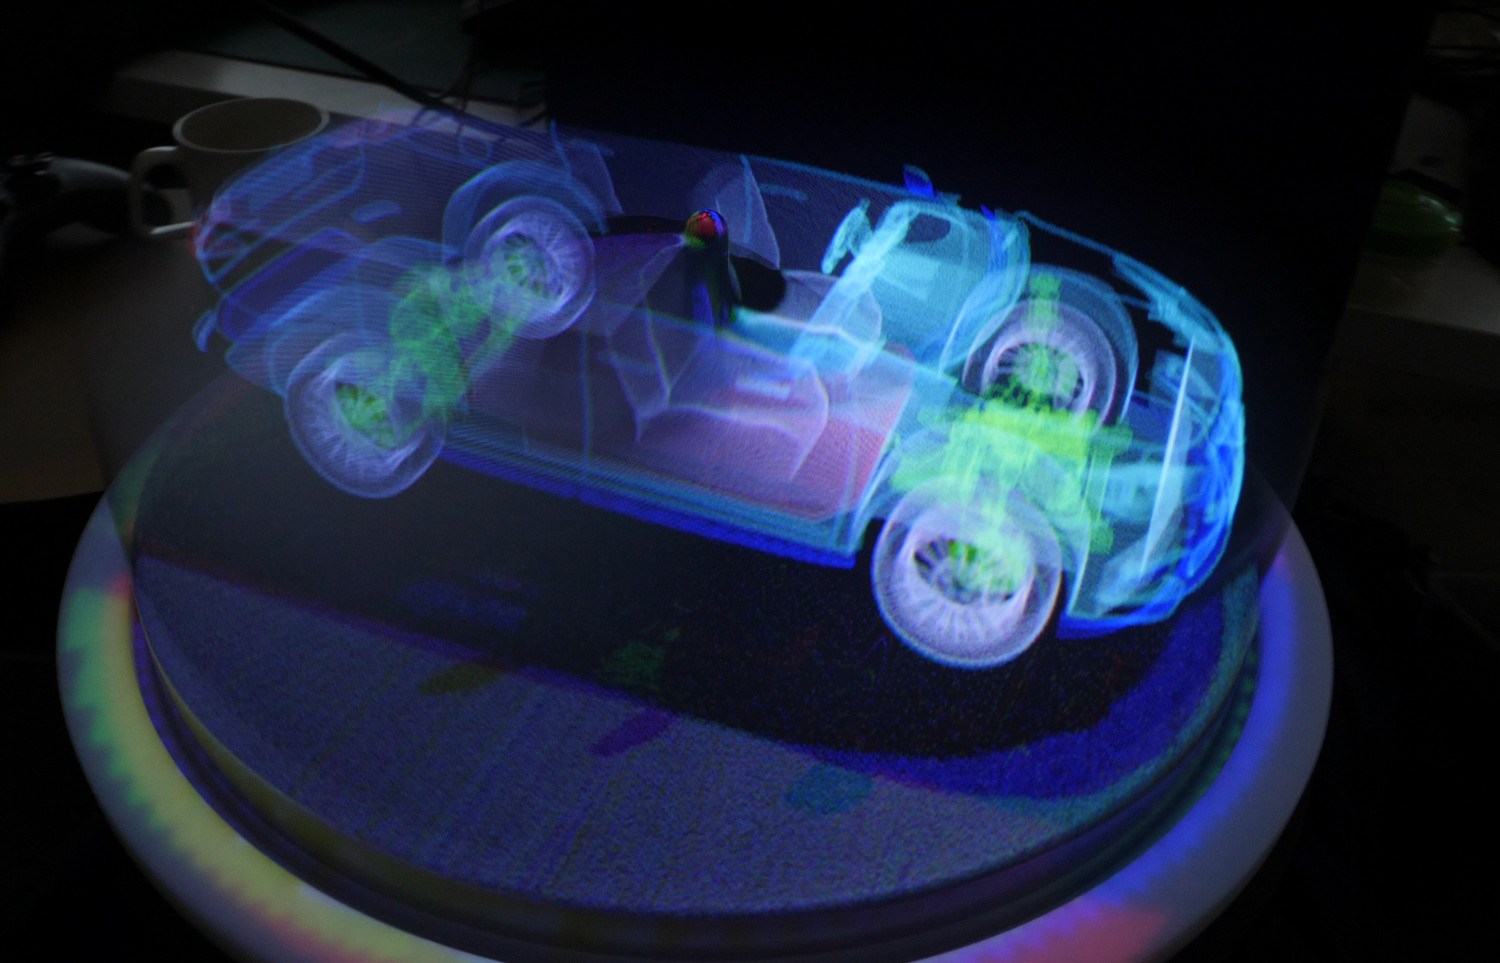
\includegraphics{./background/figures/3d/voxon.jpg}
    }
  }
  \hfill
  \pictureBox[label={fig:brightbox}]{A Volumetric Display / Holographic Signage, an LED-based persistence of vision display produced by Brightvox Inc. \cite{brightvox_2023}}{
  \adjustbox{height=4.5cm, keepaspectratio}{
    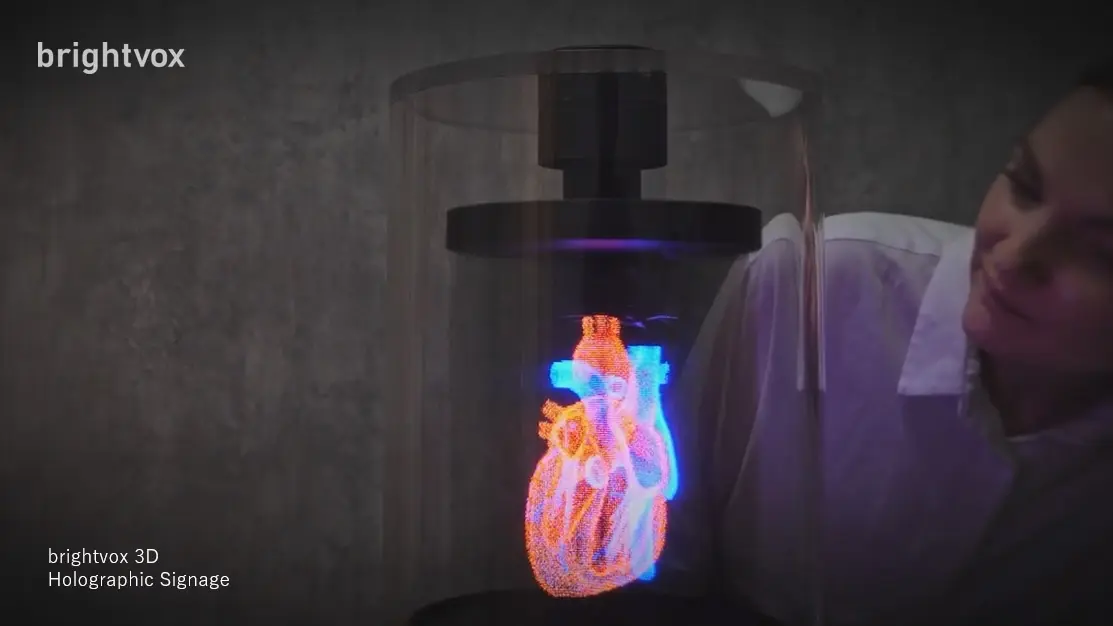
\includegraphics{./background/figures/3d/brightvox.png}
    }
  }
\end{invisBox}

\subsection{Static Volume Displays}
Static volume displays are another category. They employ a static transparent medium that when interacted with creates a 3D image. The result is that light is emitted from the display at each point in a 3D space. Techniques for achieving this range from using a 3D array of LEDs \cite{10.1145/2341931.2341937}, lasers and phosphorus gas \cite{https://doi.org/10.1002/anie.202003160}, or a transparent laser-induced damaged medium that can be projected into \cite{10.1145/1179849.1179982}. There has been research into photon-activated dye \cite{Patel2017} and even quantum dot-based displays \cite{Hirayama2015}. An example of one such display can be seen in Fig~\ref{fig:passive-optical}.

\subsection{Trapped Particle Displays}
Acoustic Trapping Displays displays are a relatively new category of volumetric displays. They employ a 3D array of particles that are suspended in air using acoustic levitation. \cite{10.1063/1.5113467} \cite{Hirayama2019} This is achieved by using an array of ultrasonic transducers to create a standing wave that can trap particles in the nodes of the wave. By moving the nodes of the wave through a 3D space and illuminating the particles with light, a 3D image can be created. This technique is still in its infancy and can struggle to provide a convincing persistence of vision effect. Another direction some researchers have taken is to use a photophoretic trap to trap particles in air \cite{Smalley2018}. The advantage of this sort of display is that space that is not being used to display an object is empty and can be passed through. This is in contrast to swept volume displays/most static volume displays where the space not being used to display an object is filled with the display's hardware. An example of one such display can be seen in Fig~\ref{fig:acoustic}.

\begin{invisBox}
	\pictureBox[label={fig:passive-optical}]{Columbia University's passive optical scattering volumetric display \cite{10.1145/1179849.1179982}}{
	  \adjustbox{height=5.25cm, keepaspectratio}{
		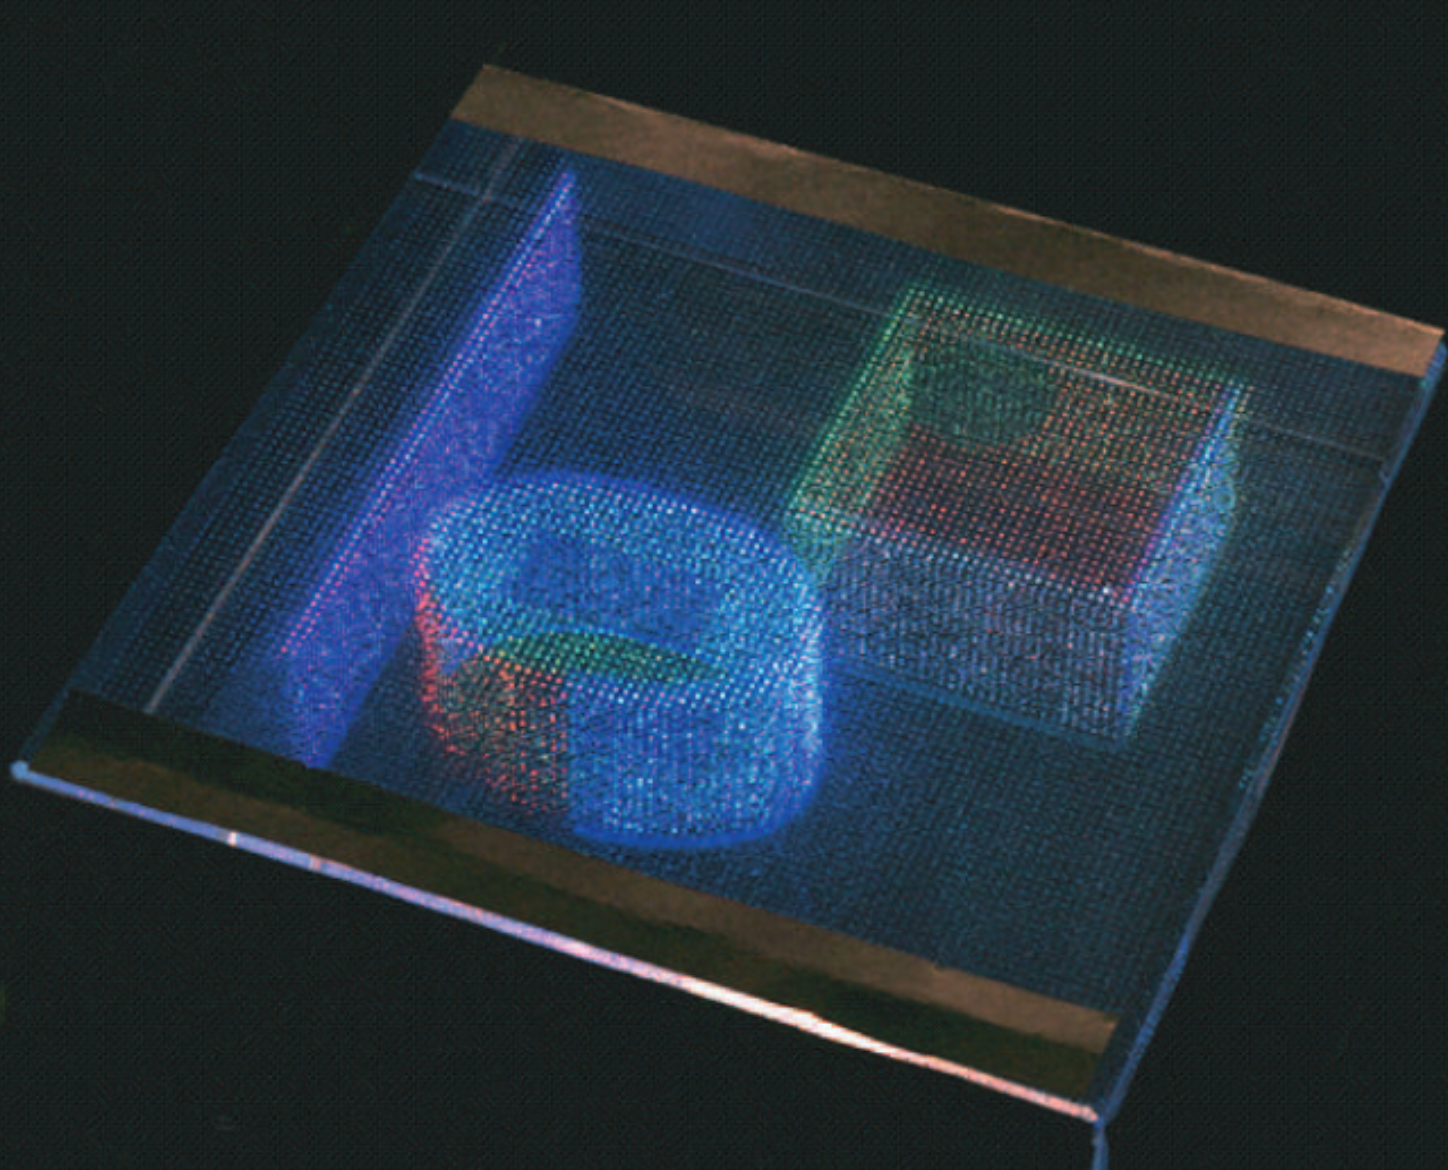
\includegraphics{./introduction/figures/passive optical scatterers.png}
	  }
	}
	\hfill
	\pictureBox[label={fig:acoustic}]{Bristol University's acoustic trapping volumetric display \cite{10.1063/1.5113467}}{
	\adjustbox{height=5.75cm, keepaspectratio}{
	  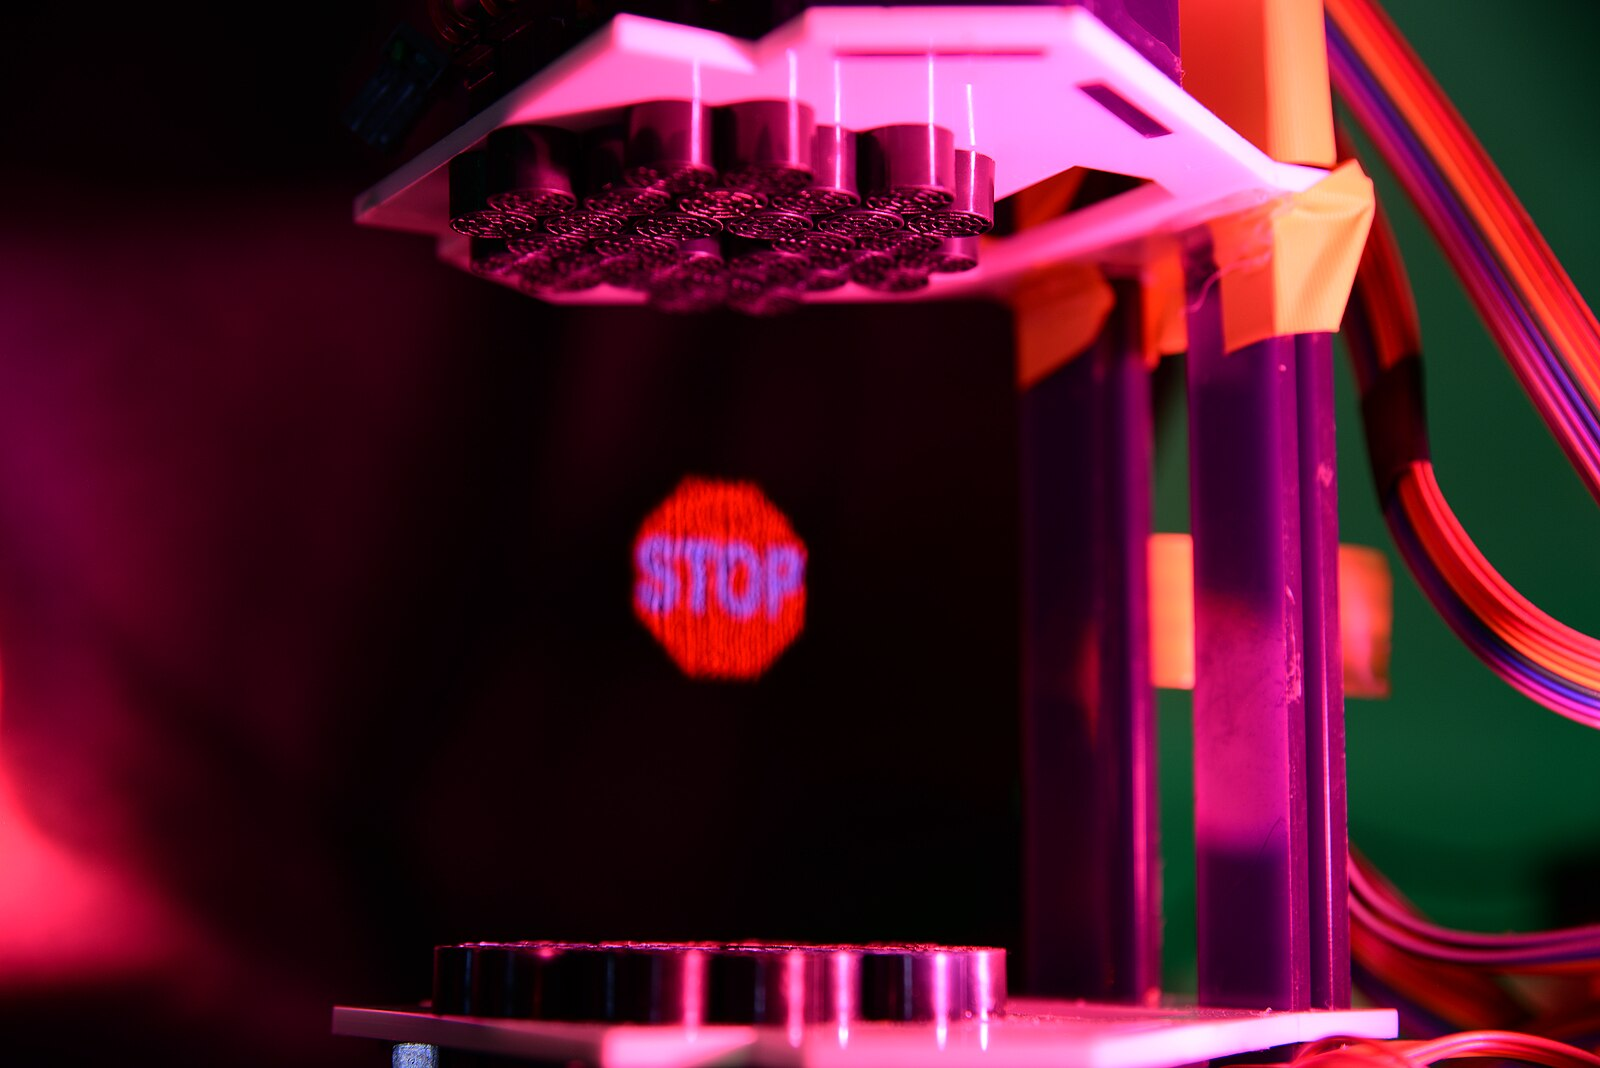
\includegraphics{./introduction/figures/acoustophoretic display.jpg}
	  }
	}
	\end{invisBox}
\subsection{Issues}

Volumetric displays often require custom/cutting-edge hardware (e.g. extremely high refresh rate projectors,  transparent micro LEDs, complex laser systems) which makes them expensive, difficult to manufacture and calibrate and not widely available. For example, the Voxon VX1, one of the few if only commercially available volumetric displays costs, \$11,700 USD \cite{noauthor_products_nodate} per unit. \\

Volumetric displays are also held back by their inherent high bandwidth requirements: To render objects in real-time at equivalent resolutions to current 2D displays while taking a raw voxel stream (as opposed to calculating voxels on hardware from primitive shapes) has an extremely high bandwidth requirement. If we want to render at \texttt{60fps} on a $4096 \times 2160 \times 1080$ voxel display with \texttt{24 bit} color, it would require a bandwidth of $1.37 \times 10^3$ bits per second/13.7 terabits per second which is orders of magnitude higher than what a normal display requires. To achieve that currently would require about 170 state-of-the-art Ultra High Bit Rate (UHBR) (80 gigabit) DisplayPort cables simultaneously. It was predicted in 2021 \cite{LAM2021050011} that due to these limitations and based on the historic trends of bandwidth in commercially available displays, volumetric displays will only become feasible in 2060 at the earliest. There are ways to reduce this bandwidth requirement through compression and other techniques \cite{4487481} but this still provides a major issue. \\

\subsection{Volumetric Screen Simulations}
Because of these issues, there has been some research into simulating volumetric displays. One commonly used method is the so-called fish tank virtual reality (FTVR) display \cite{10.1145/169059.169066} which has been commonly used to simulate volumetric displays, \cite{10.1145/3281505.3281540}, \cite{Zabarauskas2012}. A FTVR comprises a singular or set of 2D displays that are positioned in front of a user. The viewer's eyes are tracked in 3D space and the image on the displays is adjusted accordingly so that there appears to be a 3D image present in front of them. This is a relatively cheap and easy way to simulate a volumetric display, but it has some major drawbacks. The user is limited to a single focal depth and is limited to a single vergence (This can be fixed by wearing glasses to filter different images to each eye providing a stereo view \cite{5701756}). This system is also limited to just a single user at a time unless image filtering is used. 

Another approach that has been taken is to take advantage of virtual reality (VR) headsets. VR headsets are a relatively cheap and easy way to simulate a volumetric display. They are also able to provide a stereo view and can be used by multiple users at once \cite{10.1145/3290605.3300763}.
\label{sect:3d}
\section{Nix/NixOS}
\subsection{Introduction to Nix}

\textbf{Nix} \cite{dolstra2004nix} is an open-source, "purely functional package manager” used in Unix-like operating systems to provide a functional and reproducible approach to package management. Started in 2003 as a research project Nix \cite{dolstra2006purely} is widely used in both industry \cite{NixCommunityNixOSWiki} and academia \cite{10.1145/3152493.3152556} \cite{https://doi.org/10.1002/qua.26872} \cite{LHCbNix}, and its associated public package repository \texttt{nixpkgs} \cite{NixPkgs} as of Jan 2024 has over 80,000 unique packages making it the largest up-to-date package repository in the world  \cite{Marakasov_2024}. Out of Nix has also grown \textbf{NixOS} \cite{10.1145/1411204.1411255} a Linux distribution that is conceived and defined as a deterministic and reproducible entity that is declared functionally and is built using the \textbf{Nix} package manager. \\

Nix packages are defined in the \textbf{Nix Language} a lazy functional programming language where packages are treated like purely functional values that are built by side effect-less functions and once produced are immutable. Packages are built with every dependency down to the \texttt{ELF} interpreter and \texttt{libc} (C standard library) defined in nix. All packages are installed in the store directory, typically \texttt{/nix/store/} by their unique hash and package name as can be seen in Fig~\ref{fig:nix-store-path} as opposed to the traditional Unix Filesystem Hierarchy Standard (FHS).

%% Nix Store Path
\begin{figureBox}[label={fig:nix-store-path}, width=0.8\linewidth]{Nix Store Path}
  \begin{tabbing}
    \={\color{Purple}\texttt{/nix/store/}}\={\color{RoyalBlue}\texttt{sbldylj3clbkc0aqvjjzfa6slp4zdvlj}}-\={\color{Orange}\texttt{hello-2.12.1}} \\
    \>\small{Prefix} \>\small {Hash part} \>\small {Package name}
  \end{tabbing}
\end{figureBox}

Package source files, like tarballs and patches, are also downloaded and stored with their hash in the store directory where packages can find them when building. Changing a package's dependencies results in a different hash and therefore location in the store directory which means you can have multiple versions or variants of the same package installed simultaneously without issue. This design also avoids "DLL hell" by making it impossible to accidentally point at the wrong version of a package. Another important result is that upgrading or uninstalling a package cannot ever break other applications. \\

Nix builds packages in a sandbox to ensure they are built exactly the same way on every machine by restricting access to nonreproducible files, OS features (like time and date), and the network \cite{nixcon-sandboxs}. A package can and should be pinned to a specific NixOS release (regardless of whether you are using NixOS or just the package manager). This means that once a package is configured to build correctly it will continue to work the same way in the future, regardless of when and where it is used and it will never not be able to be built. \\

These features are extremely useful for scientific work, CERN uses Nix to package the LHCb Experiment because it allows the software "to be stable for long periods (longer than even long-term support operating systems)" and it means that as Nix is reproducible; all the experiments are completely reproducible as all bugs that existed in the original experiment stay and ensure the accuracy of the results \cite{LHCbNix}. \\

To create a package Nix evaluates a \textbf{derivation} which is a specification/recipe that defines how a package should be built. It includes all the necessary information and instructions for building a package from its source code, such as the source location, build dependencies, build commands, and post-installation steps. By default, Nix uses binary caching to build packages faster, the default cache is \texttt{cache.nixos.org} is open to everyone and is constantly being populated by CI systems. You can also specify custom caches. The basic iterative process for building Nix packages can be seen in Fig~\ref{fig:nix-derivation-loop}.

\begin{figureBox}[label = {fig:nix-derivation-loop}, width=0.8\linewidth]{Nix Build Loop}
  { \footnotesize
  \begin{enumerate}
    \item A hash is computed for the package derivation and, using that hash, a Nix store path is generated, e.g \nixstore[sbldylj3clbkc0aqvjjzfa6slp4zdvlj]{hello-2.12.1}.
    \item  Using the store path, Nix checks if the derivation has already been built. First, checking the configured Nix store e.g {\color{Purple}\texttt{/nix/store/}} to see if the path e.g {\color{RoyalBlue}\texttt{sbldylj3clbkc0aqvjjzfa6slp4zdvlj}}-{\color{Orange}\texttt{hello-2.12.1}} already exists. If it does, it uses that, if it does not it continues to the next step.
    \item Next it checks if the store path exists in a configured binary cache, this is by default \texttt{cache.nixos.org}. If it does it downloads it from the cache and uses that. If it does not it continues to the next step.
    \item Nix will build the derivation from scratch, recursively following all of the steps in this list, using already-realized packages whenever possible and building only what is necessary. Once the derivation is built, it is added to the Nix store.
  \end{enumerate}
  }
\end{figureBox}

\subsection{Example of a Nix package}

To give an example of what a Nix package might look like. We have created a flake (one method of defining a package) in Listing~\ref{list:nix-flake} that builds a version of the classic example package "hello". 

\codeBoxFile[label = {list:nix-flake}]{nix}{./background/code/hello.nix}{flake.nix}

To dive deeper into what each line does we have given a breakdown below for the \texttt{flake.nix} \\
{ \small
\begin{itemize}
  \item \textbf{Line 2:} We have specified that we want to build our flake with the stable \textbf{nix channel} \texttt{nixos-23.11}, the most recent channel at the time of writing. This "channel" is just a release branch on the \texttt{nixpkgs} GitHub repository. Channels do receive conservative updates such as bug fixes and security patches but no major updates after the initial release. The first time we build the hello package from our \texttt{flake.nix} a \texttt{flake.lock} is automatically generated that pins us to a specific revision of \texttt{nixos-23.11}. Our built inputs will not change until we relock our flake to either a different revision of \texttt{nixos-23.11} or a new channel entirely. 

  \item \textbf{Line 5:} Here we define \texttt{outputs} as a function that accepts, \texttt{self} (the flake) and \texttt{nixpkgs} (the set of packages we just pinned to on line 2). Nix will resolve all inputs, and then call the \texttt{output} function.
  
  \item \textbf{Line 6:} Here we specify that we are defining the default package for users on \texttt{x86\_64-linux}. If we tried to build this package on a different CPU architecture like for example ARM (\texttt{aarch64-linux}) the flake would refuse to build as the package has not been defined for ARM yet. If we desired we could fix this by adding a \texttt{defaultPackage.aarch64-linux} definition.

  \item \textbf{Line 7-9:} Here we are just defining a shorthand way to refer to x86 Linux packages. This syntax is similar if not identical to Haskell.

  \item \textbf{Line 10:} Here we begin the definition of the derivation which is the instruction set Nix uses to build the package.
  
  \item \textbf{Line 14:} We specify here that we need \texttt{gcc} in our sandbox to build our package. \texttt{gcc} here is shorthand for \texttt{gcc12} but we could specify any c compiler with any version of that compiler we liked. If you desired you could compile different parts of your package with different versions of GCC.

  \item \textbf{Line 15:} Here we are slightly abusing the configure phase to generate a hello.c file. You would usually download a source to build from with a command like \texttt{fetchurl} while providing a hash. Each phase is essentially run as a bash script. Everything inside \texttt{mkDerivation} is happening inside a sandbox that will be discarded once the package is built (technically after we garbage collect). 
  
  \item \textbf{Line 16:} Here we actually build our package
  
  \item \textbf{Line 17:} In this line we copy the executable we have generated which is currently in the sandbox into the actual package we are producing which will be in the store directory \texttt{/nix/store}. 
\end{itemize}
}
Below we have given some examples of how to run and investigate our hello package in Listing~\ref{list:nix-terminal}.

\codeBoxFile[label = {list:nix-terminal},  width=0.75\linewidth]{shell}{./background/code/hello-nix.sh}{Terminal}

In Fig~\ref{fig:dependency-graph} we can see the package dependency graph of our \texttt{hello} package. We are only dependent on 4 packages \texttt{libunistring}, \texttt{libidn2}, \texttt{xgcc}, \texttt{glibc} all of which Nix have installed and configured separately the rest of the non-nix system (assuming we are not on NixOS). 

\begin{figureBox}[label = {fig:dependency-graph}, width=0.75\linewidth]{Dependency graph}
  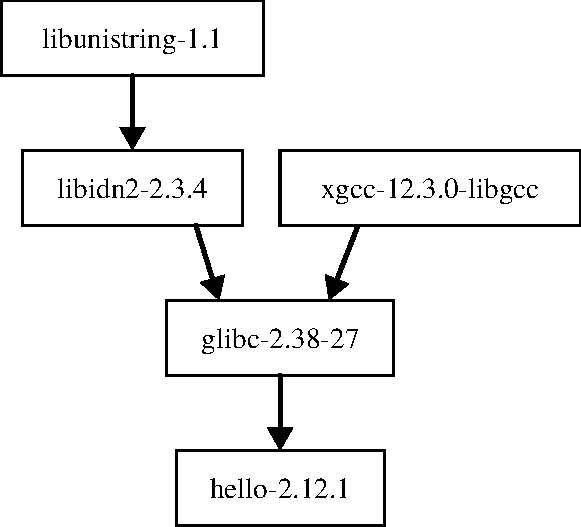
\includegraphics[width=0.7\linewidth]{./background/figures/nix/hello-pkg.pdf}
\end{figureBox}

\label{sect:nix}

%%%%%%%%%%%%%%%%%%%%%%%%%%%%%%%%%%%%
\chapter{Methods}
\section{Perspective Projection}

\begin{figureBox}[label={fig:ortho-vs-persp}, width=0.8\linewidth]{Orthographic and perspective projections}
    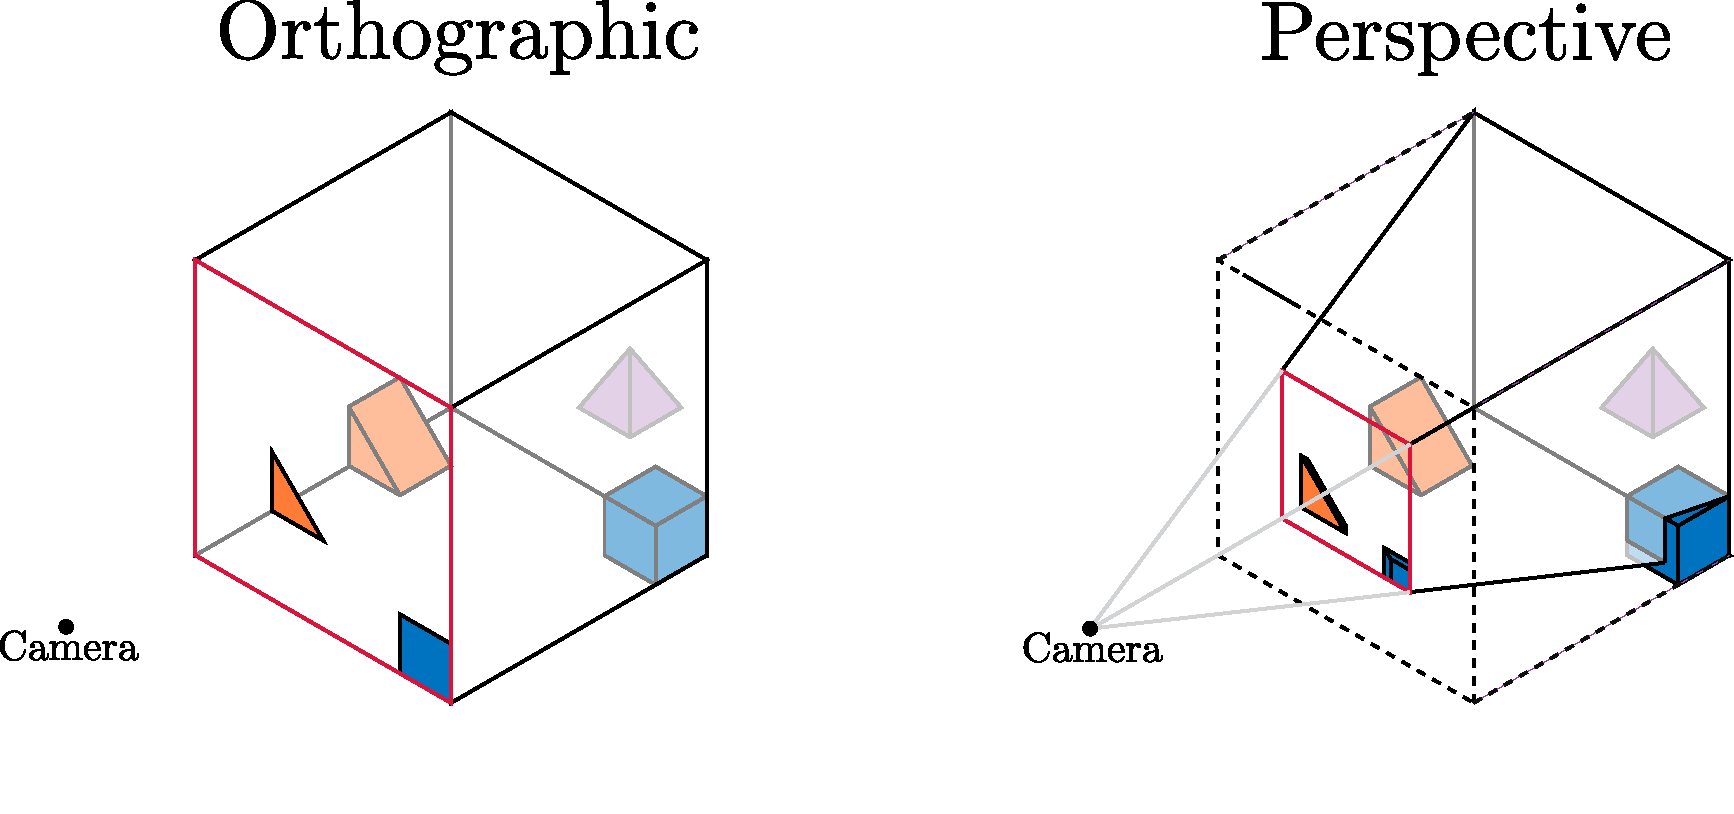
\includegraphics[width = 0.8\linewidth]{./background/figures/projection/ortho-vs-persp.pdf}
\end{figureBox}

To represent 3D objects on a 2D surface (our screen) OpenGL supports two types of projections: perspective and orthographic as seen in Fig~\ref{fig:ortho-vs-persp}. Orthographic features parallel projection lines (orthogonal to the projection plane), which means that it does not depict the effect of perspective. Distances are preserved, making it useful for technical drawings where measurements need to be precise and not skewed by perspective (All diagrams in this report are from the orthographic perspective). Unlike orthographic projection, perspective projection simulates the way the human eye perceives the world, with objects appearing smaller as they are farther from the viewpoint as the projection lines converge at a vanishing point. To create the illusion of 3D in this project we must use a perspective projection.

\subsection{Generating the perspective projection}

\begin{figureBox}[label={fig:persp-projection}, width=0.8\linewidth]{Using frustum to generate a perspective projection}
    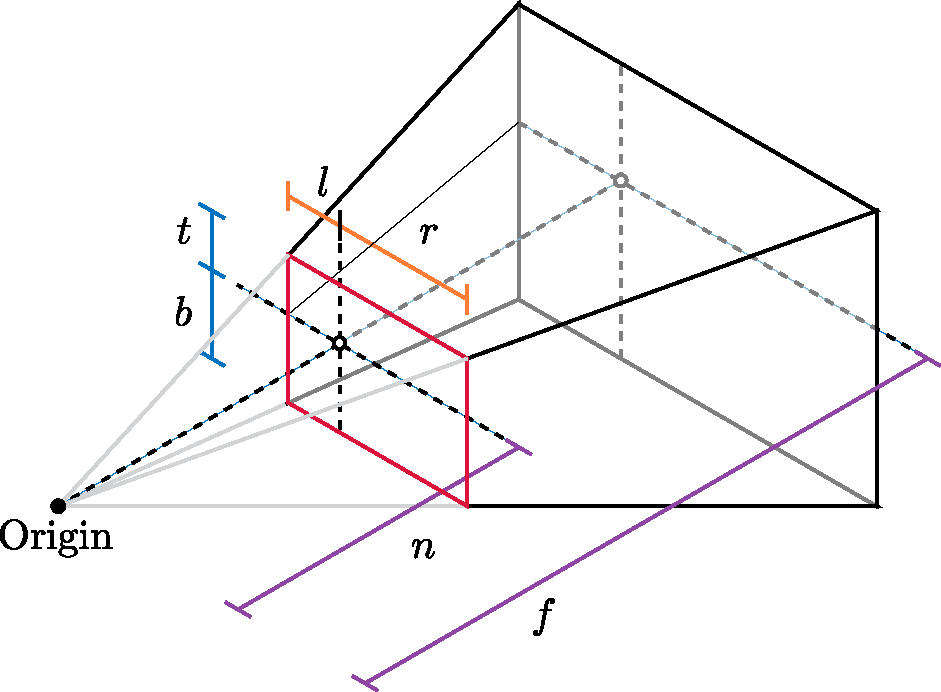
\includegraphics[width = 0.8\linewidth]{./background/figures/projection/persp-projection.pdf}
\end{figureBox}

OpenGL provides the \texttt{frustum} function as seen in Fig~\ref{fig:persp-projection} which can be used to construct a perspective matrix.     
\[
    \begin{bmatrix}
        \frac{2n}{r-l} & 0              & \frac{r+l}{r-l}  & 0                \\
        0              & \frac{2n}{t-b} & \frac{t+b}{t-b}  & 0                \\
        0              & 0              & -\frac{f+n}{f-n} & -\frac{2fn}{f-n} \\
        0              & 0              & -1               & 0                \\
    \end{bmatrix}
\] 
This maps a specified viewing frustum screen-space (with intermediate steps handled by OpenGL) \cite{hearn2004computer}. The viewing frustum is specified by six parameters: $f$, $l$, $r$, $b$, $t$, $n$ which represent left, right, bottom, top, near, and far. These parameters define the sides of the near-clipping plane, highlighted in red, relative to the origin of the coordinate system. These parameters do not represent distances or magnitudes in a traditional sense but rather define the vectors from the center of the near-clipping plane to its edges. \\


The $l$ and $r$ parameters specify the horizontal boundaries of the frustum on the near-clipping plane, with left typically being a negative value and right a positive value, defining the extent to which the frustum extends to the left and right of the origin. Similarly, the $b$ and $t$ parameters determine the vertical boundaries, with the bottom often negative and the top positive, expressing the extent of the frustum below and above the origin. \\

The $n$ and $f$ parameters are scalar values that specify the distances from the origin to the near and far clipping planes along the view direction. Altering the value of $n$ will change the angles of the lines (or vectors) that connect the corners of the near plane to the eye, effectively changing the "field of view". Changing the value $f$ affects the range of depth that is captured within the scene. \\

If we can track the position of a viewer's eye in real time then we can create the illusion of a 3D scene behind and in front of a display using \texttt{frustum}. This can be done fairly trivially following Robert Kooima's method he sets out in "Generalized Perspective Projection" to calculate $f$, $l$, $r$, $b$, $t$, $n$ as the viewer's eye moves \cite{kooima2009generalized}. \\

To encode the position and size of the screen we take 3 points, $p_a$, $p_b$ and $p_c$ which represent the lower-left, lower-right and upper-left points of the screen respectively when viewed from the front on. These points are in tracker space, the coordinate system of the device we use to track the eyes. This point can be used to generate an orthonormal basis of the screen of $s_r$, $s_u$ and $s_n$ which represents the directions up, right and normal to the screen respectively as seen in Fig~\ref{fig:perspective-screen}. We can compute these values from the screen corners as follows:
\[s_r = \frac{p_b-p_a}{||p_b-p_a||} \quad s_u = \frac{p_c-p_a}{||p_c-p_a||} \quad s_n = \frac{s_r\times s_u}{||s_r \times s_u||}\]

\begin{figureBox}[label={fig:perspective-screen}, width=0.8\linewidth]{Defining a screen in 3D space}
    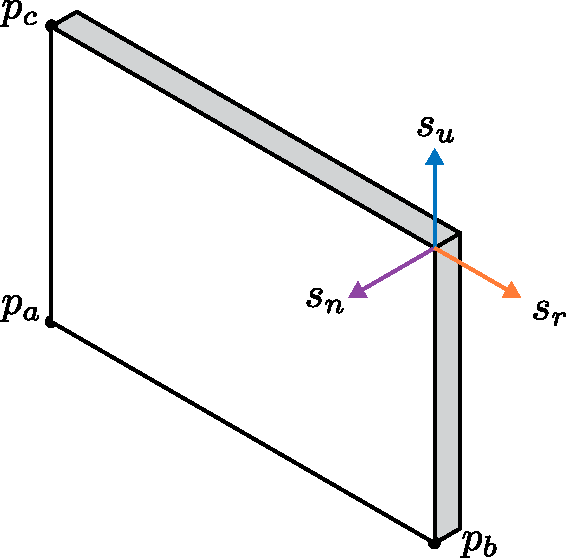
\includegraphics[width = 0.3\linewidth]{./background/figures/projection/screen.pdf}
\end{figureBox}

Introducing the viewer's eye which we will refer to as $p_e$. We can draw three vectors $v_a$, $v_b$, $v_c$ from the viewers eye $p_e$ to the corners of the screen $p_a$, $p_b$, $p_c$ as seen in Fig~\ref{fig:screen-extents}. In the diagram, we also have labeled the components of each of these vectors in the basis of the screen. We can compute these as follows:
\[ v_a = p_a - p_e \quad v_b = p_b - p_e \quad v_c = p_c - p_e\] 

To calculate the required values for \texttt{frustum} we must first find the point where a line drawn perpendicular to the plane of the screen that passes through $p_e$ strikes the plane of the screen. We refer to this point as the {\it screen-space-origin}, it is worth noting that this point can lie outside the screen (the rectangle bounded by $p_a$, $p_b$, $p_c$). We can find the distance of the {\it screen-space-origin} from the eye $p_e$ by taking its component of $v_a$, $v_b$, $v_c$ in the screen basis vector $s_n$, however, as $s_n$ is in the opposite direction we must invert it. Similarly, we can calculate $t$ by taking the component of $v_c$ in the basis vector $s_u$, $b$ by $v_b$ in $s_u$, $l$ by $v_c$ in $s_r$ and lastly $r$ by $v_b$ in $s_r$. We can compute these as follows:
\[ d= -(s_n \cdot v_a) \quad l = (v_c \cdot s_r) \quad r = (v_b \cdot s_r) \quad b = (v_c \cdot s_u) \quad t = (v_b \cdot s_u) \]

\begin{figureBox}[label={fig:screen-extents}, width=0.8\linewidth]{Screen Intersection with view}
    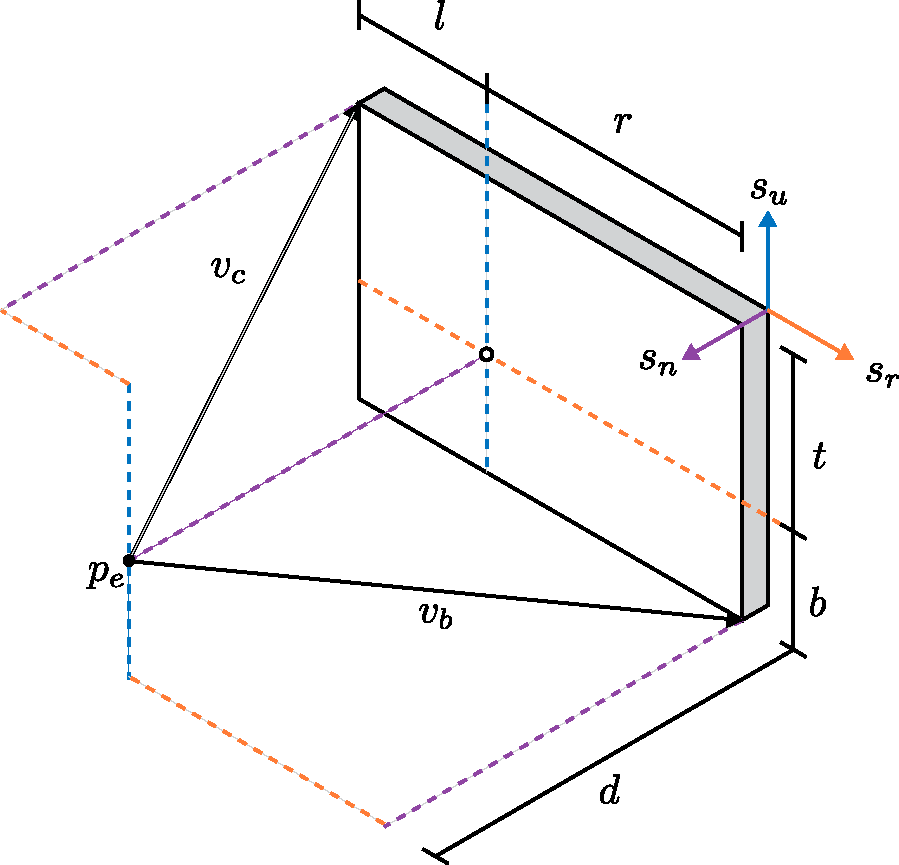
\includegraphics[width = 0.5\linewidth]{./background/figures/projection/eye-projection.pdf}
\end{figureBox}

We can now generate a projection matrix by calling \texttt{frustum} using $d$ as our near-clipping plane distance $n$ with an arbitrary value for the far-clipping plane $f$. Furthermore, we have now successfully generated our viewing frustum but we still have two problems. Firstly our frustum has been defined in tracker space so is pointed in the direction of our camera not the normal of our screen. We can remedy this problem by using a rotation matrix M to align our frustum with $s_n$, $s_u$ and $s_r$, the basis of our screen as seen in Fig~\ref{fig:basis-change}. M is defined as follows:
\[
    \begin{bmatrix}
        v_{rx} & v_{ry} & v_{rz} & 0 \\
        v_{ux} & v_{uy} & v_{uz} & 0 \\
        v_{nx} & v_{ny} & v_{nz} & 0 \\
        0      & 0      & 0      & 1 \\
    \end{bmatrix}
\]

\begin{figureBox}[label={fig:basis-change}, width=0.8\linewidth]{Moving the frustum from tracker space to screen space}
    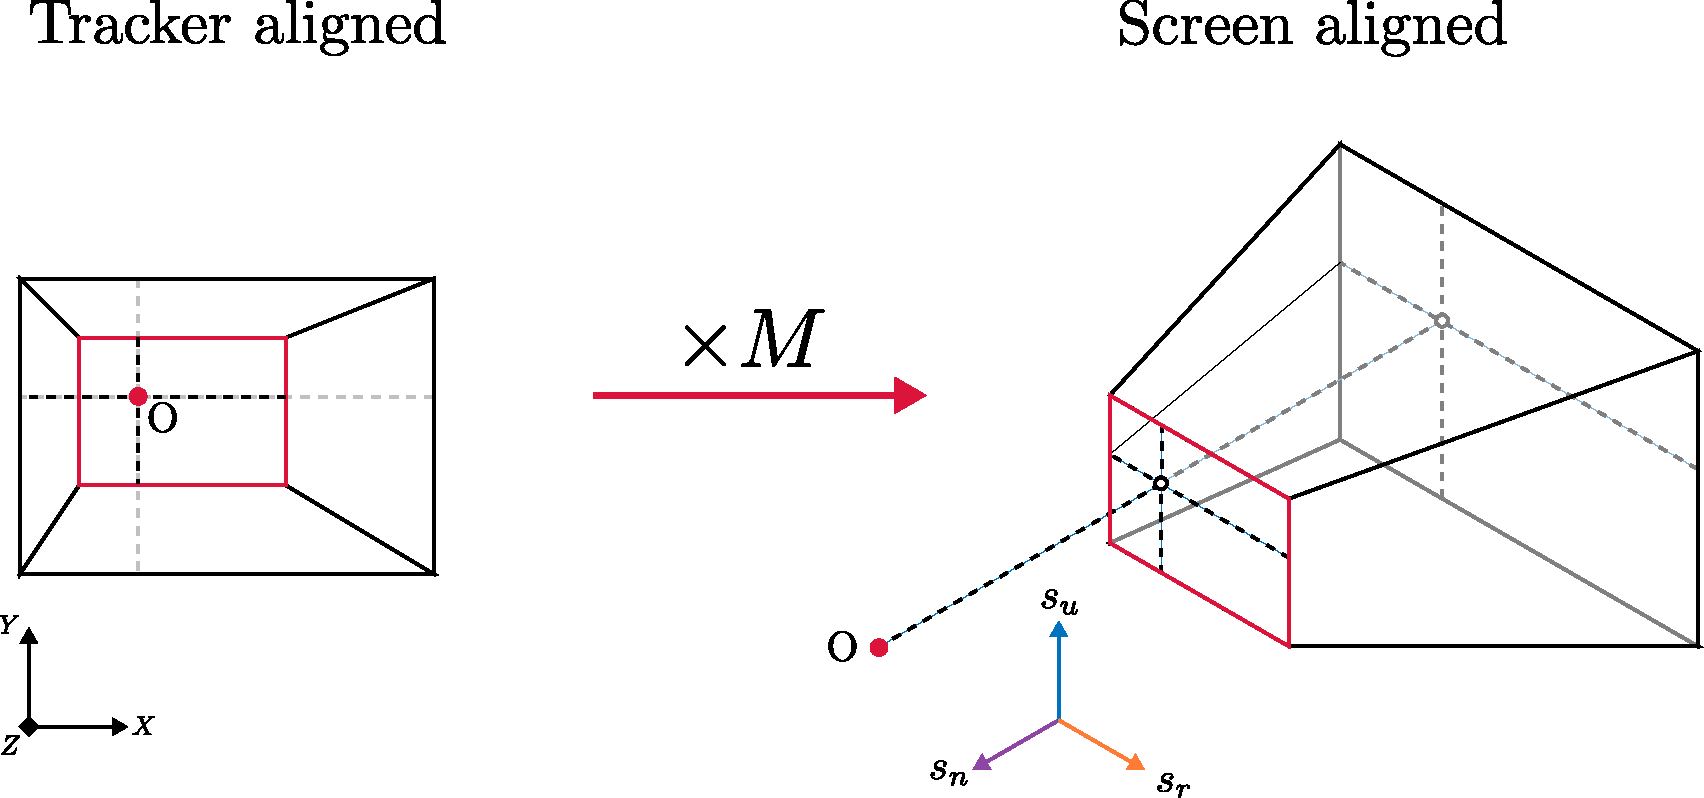
\includegraphics[width = 0.8\linewidth]{./background/figures/projection/realignment.pdf}
\end{figureBox}

The second problem we have is that we want our projection matrix to move around with the viewer's eye however the mathematics of perspective projection disallow this, with the camera forever trapped at the origin. To translate our viewing frustum to our eye position we must instead translate our eye position (and the whole world) to the apex/origin of our frustum. This can be done with a translation matrix $T$ as seen in Fig~\ref{fig:frust-translation}. $T$ can be generated with the OpenGL function \texttt{translate} where we want to offset it by the vector from our Origin to the viewers eye $p_e$. T is defined as follows:
\[
    \begin{bmatrix}
        1 & 0 & 0 & -p_{ex} \\
        0 & 1 & 0 & -p_{ey} \\
        0 & 0 & 1 & -p_{ez} \\
        0 & 0 & 0 & 1       \\
    \end{bmatrix}
\]

\begin{figureBox}[label={fig:frust-translation}, width=0.8\linewidth]{Translating the viewing frustum to sit inside the screen}
    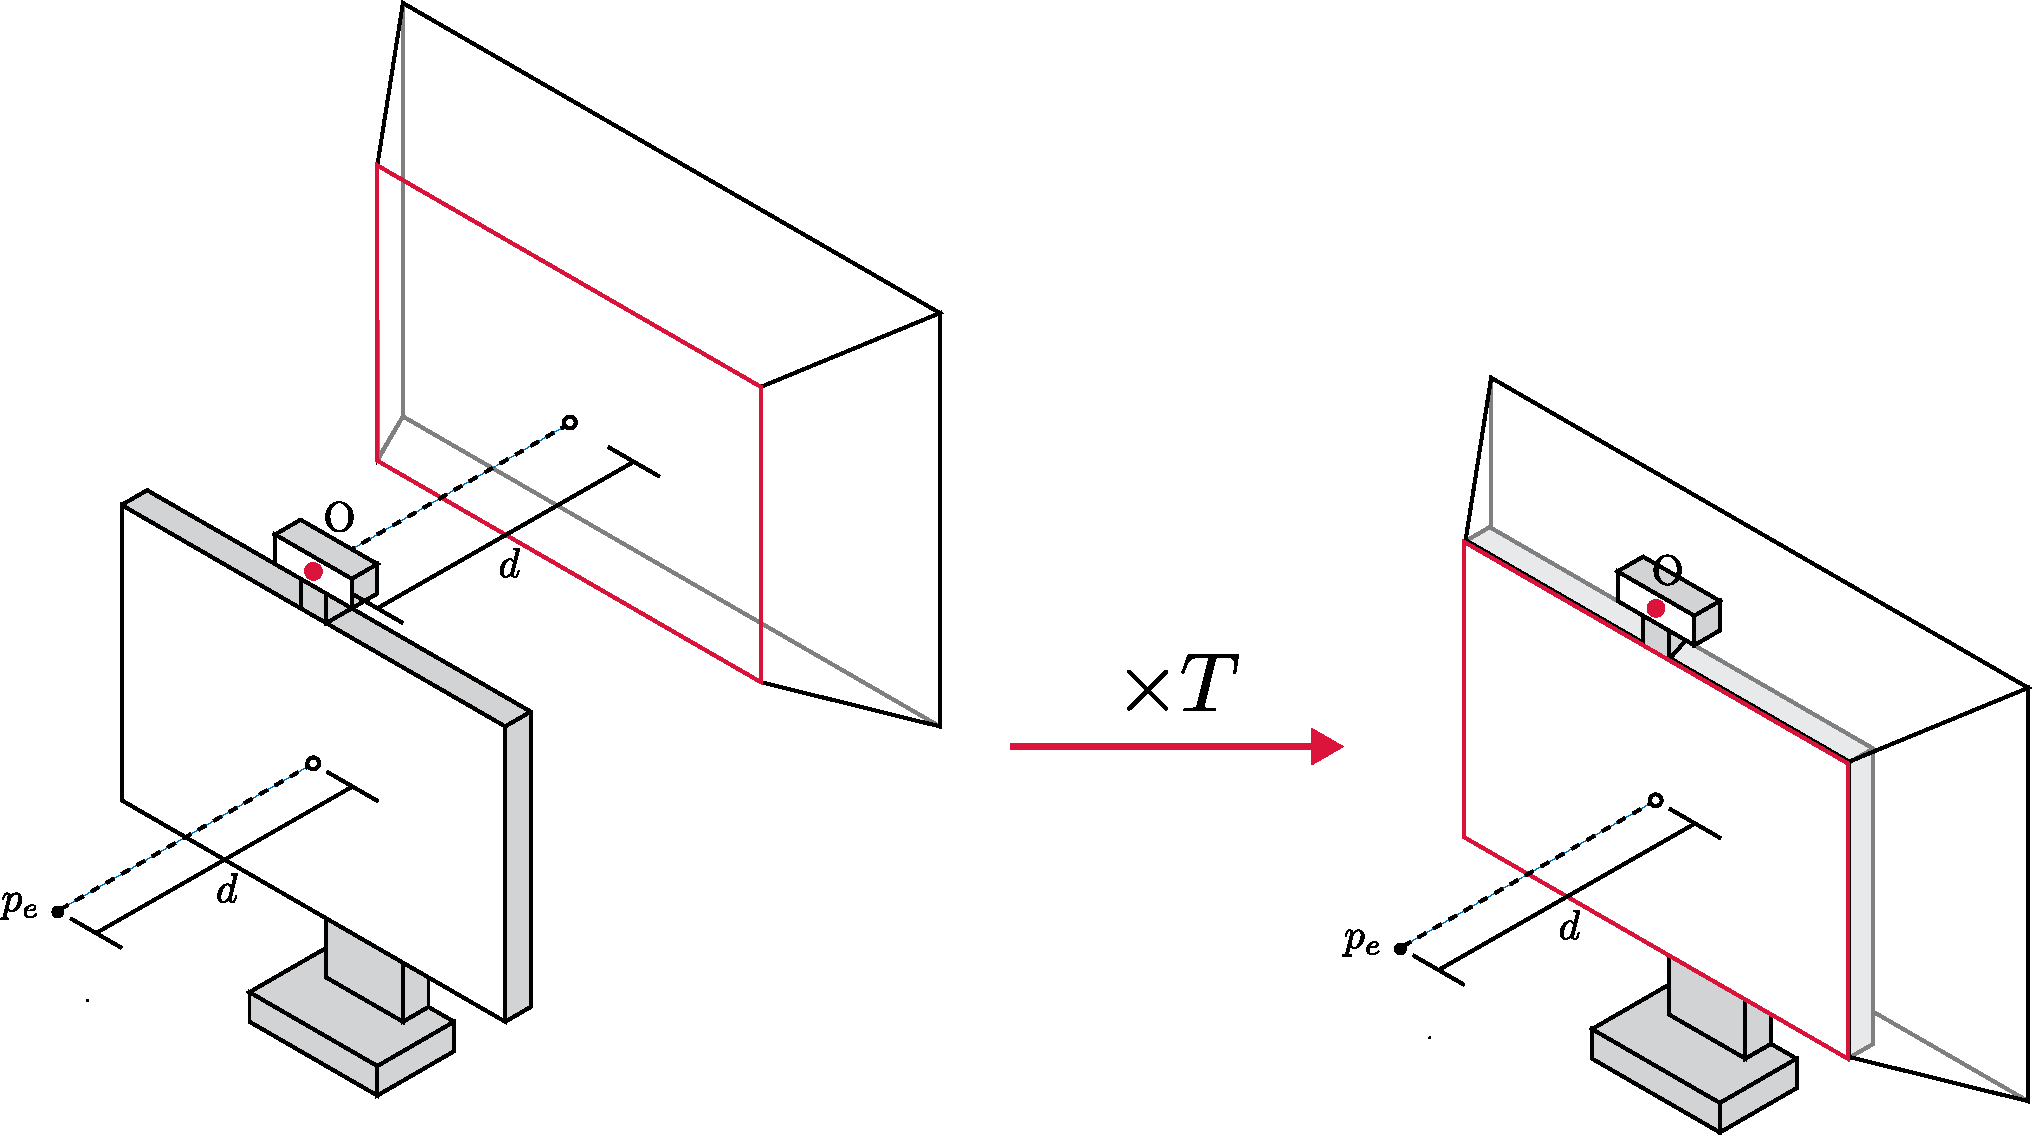
\includegraphics[width = 0.8\linewidth]{./background/figures/projection/frust-translation.pdf}
\end{figureBox}

We now have a working method for projecting virtual objects behind our screen onto our screen however it is also possible if we desire to project objects in front of the screen onto the screen as well as long as they lie within the pyramid formed between the edges of the screen and the viewer's eye. We can use similar triangles to scale the near-clipping plane from the plane of the screen to a small distance $n$ from our eye as seen in Fig~\ref{fig:extending-near}. Furthermore, we now have scaled-down values of $t$, $b$ $l$ and $r$ we can use for our new viewing frustum which we call $t_n$, $b_n$ $l_n$ and $r_n$. They are defined as follows:
\[
    l_n = (v_c \cdot s_r) \frac{n}{d} \quad r_n = (v_b \cdot s_r) \frac{n}{d} \quad b_n = (v_c \cdot s_u) \frac{n}{d} \quad t_n = (v_b \cdot s_u) \frac{n}{d}
\]

So our final viewing frustum takes in frustum extents $t_n$, $b_n$ $l_n$ and $r_n$ and $n$ and $f$ defining the distances to the near and far clipping plane.
\begin{figureBox}[label={fig:extending-near}, width=0.8\linewidth]{Extending the near plane to not clip out objects in front of the screen}
    \centering
    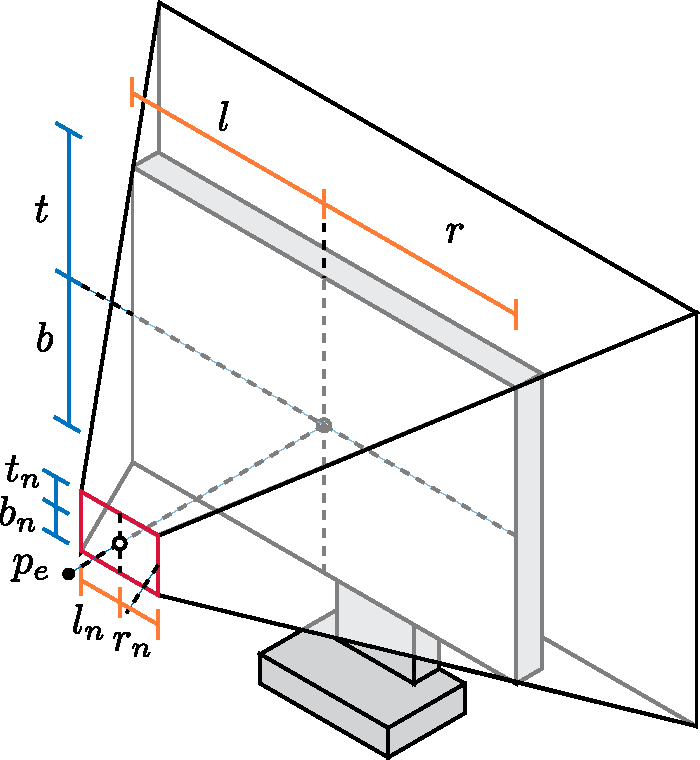
\includegraphics[width = 0.5\linewidth]{./background/figures/projection/extending-near.pdf}
\end{figureBox}

Following these steps, we can create an accurate projective providing the perspective we would expect to see if there was a scene in front and behind our screen. 

\subsection{Sample code}
Below we have attached some sample code of a function implementing the process we just described which is self-explanatory.

\codeBoxFile{cpp}{./background/code/projection.cpp}{projection.cpp, Sample code for creating the 3D illusion projection}

\label{sect:projection}

%%%%%%%%%%%%%%%%%%%%%%%%%%%%%%%%%%%%
\chapter{Implementation}
\section{Overview}

Building a Volumetric Simulator from scratch was a complex task that required the integration of various technologies and components. The most significant parts of the system are listed below, and we will discuss them in more detail in the following implementation sections.

\begin{itemize}[itemsep=-0.15em, label={}]
	\item \textbf{Simulator}: The simulator (\texttt{libvolsim.so}) is a shared library written in C++ that provides a graphical interface creating the illusion of a 3D display that can be interacted with.
	      \begin{itemize}[itemsep=-0.15em]
		      \item \textbf{Renderer Subsystem}: The rendering system is responsible for displaying the volumetric scene and the virtual objects within it. It uses OpenGL to render the scene based on user positional data from the tracking system, thus creating the illusion of 3D.
		      \item \textbf{Tracking Subsystem}: The tracking system monitors the user's hands and eyes within the scene. It employs machine learning models and a depth camera to track the user's head and eyes.
	      \end{itemize}
	\item \textbf{User Study CLI}: The User Study CLI (command-line interface) orchestrates the running of the simulator and stores the results of the user study in a MongoDB database. It also provides functionality to automatically analyse study data. This component is written in Python.
	\item \textbf{Build System}: The build system compiles the simulator and rendering system, as well as manages the execution of the user study. It uses Nix to handle dependencies and build the system in a declarative manner.
\end{itemize}

The user interacts with the \texttt{Study CLI}, to orchestrate running simulations by invoking the simulator's shared library \texttt{libvolsim.so}. The simulator returns its results/logs to the User Study CLI (in JSON format), which then stores the data in a MongoDB database. The User Study CLI can subsequently be used to analyse the results. A schematic of the system layout is shown in Fig~\ref{fig:system-layout}.

\begin{figureBox}[label={fig:system-layout}, width=1.0\linewidth]{Two examples of using our system}
    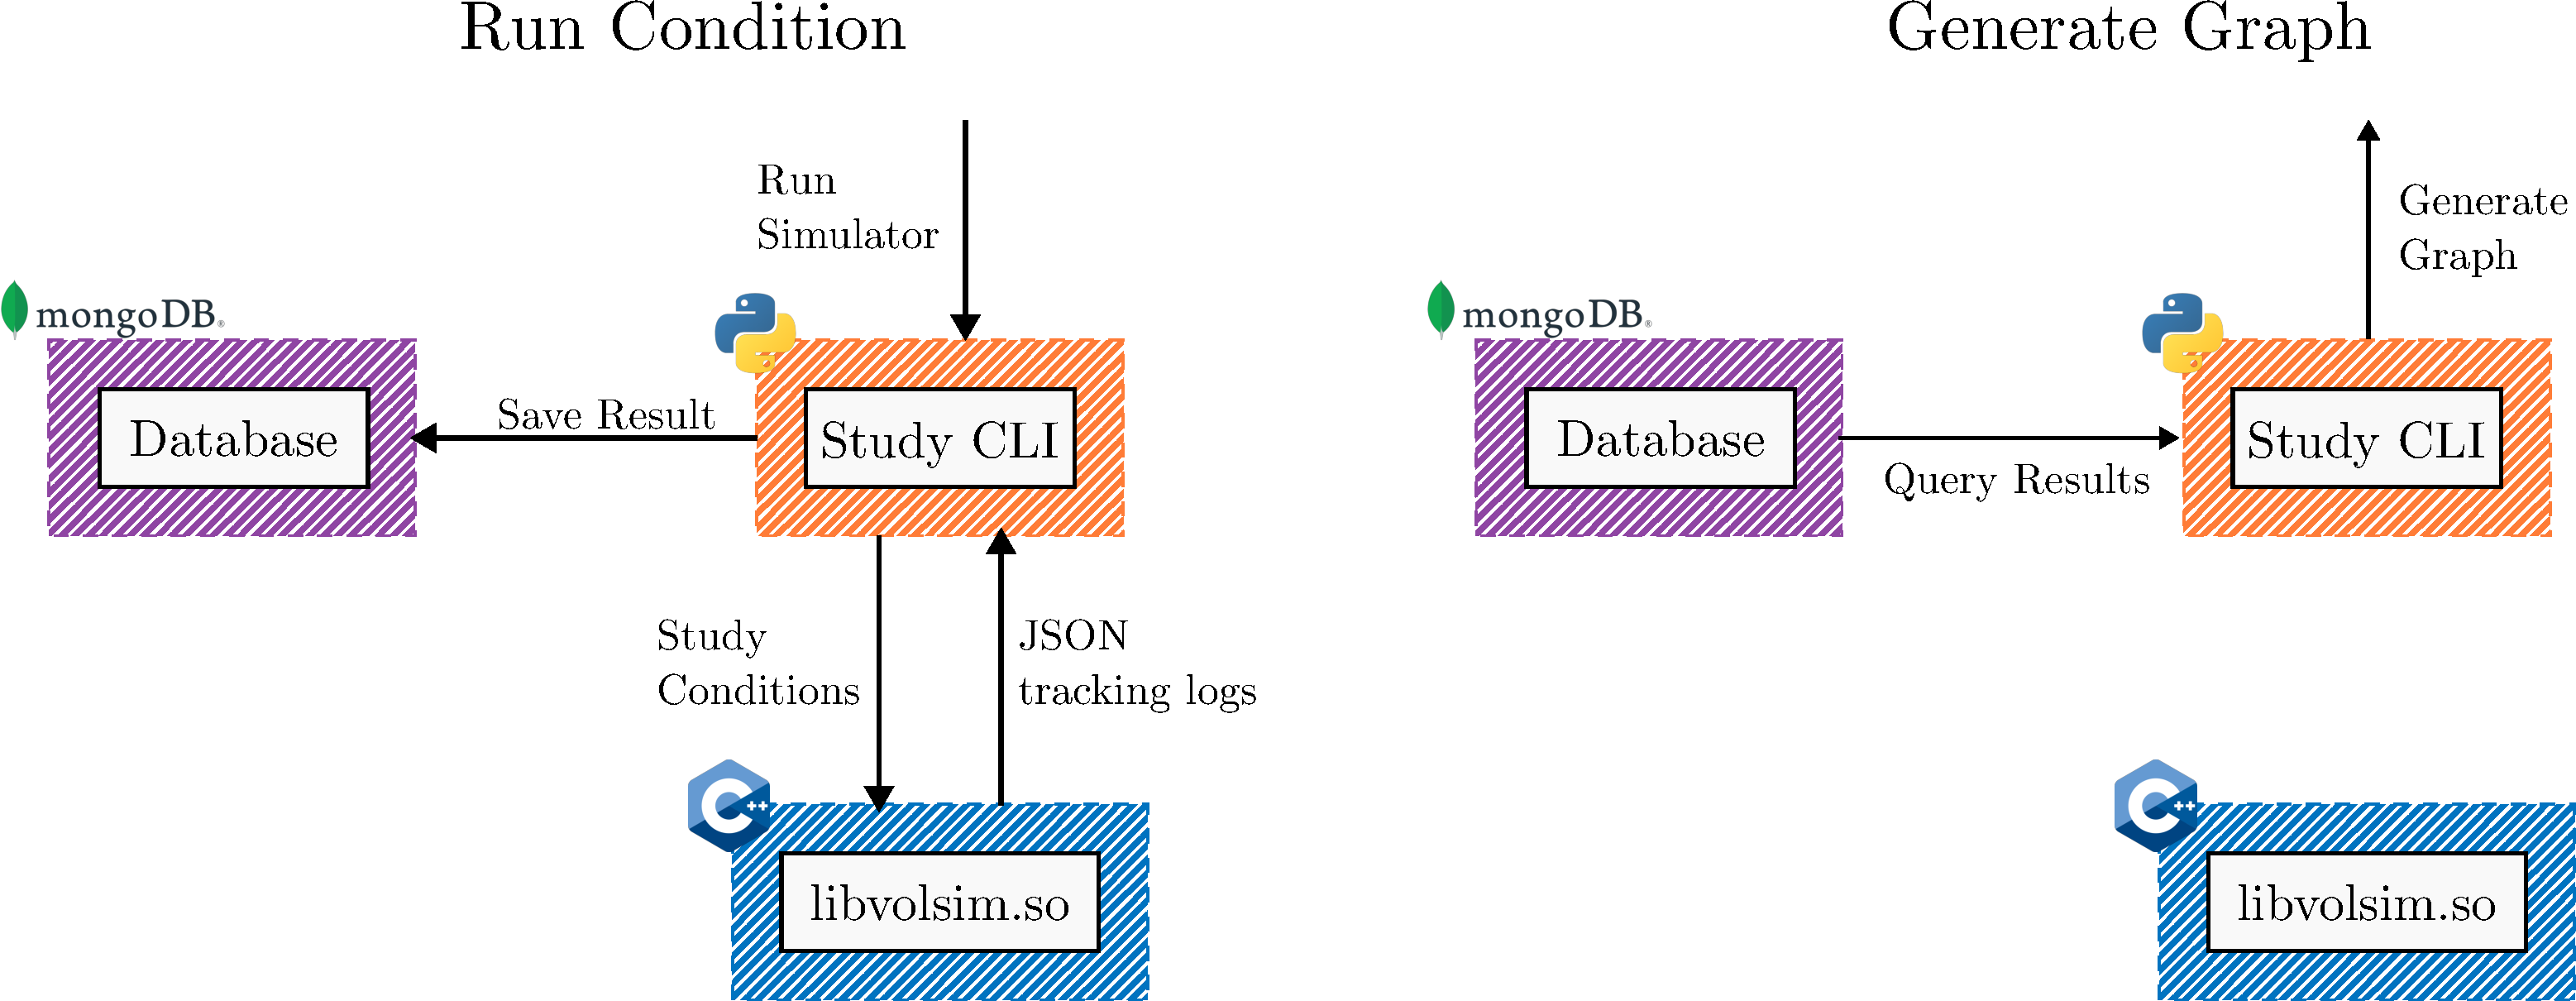
\includegraphics[width = 0.9\linewidth]{./implementation/figures/overall-system.pdf}
\end{figureBox}
\label{sect:overview}
\section{Build System}
\begin{enumerate}
	\item CUDA support
	\item Model loading support
	\item Easily Portable
	\item Having to package connect and mediapipe.
\end{enumerate}
\label{sect:buildsystem}
\section{Rendering System}
\subsection{Introduction}
The rendering system is a key component of the Volumetric Simulator, responsible for displaying models in a manner that makes them appear three-dimensional. It needs to be fast and responsive to maintain the illusion of 3D.

\subsection{OpenGL}

Our project requires the rendering system to render 3D models in real-time with low latency and a high frame rate. We decided to use OpenGL \cite{woo1999opengl} to achieve this due to its low-level control over the rendering pipeline and cross-platform compatibility. \\

We briefly considered using fully fledged game engines like Unity \cite{noauthor_unity_nodate} or Unreal Engine \cite{unrealengine}, but ultimately decided against them due to the significant overhead and lack of fine control over the rendering pipeline. Additionally, we utilised the OpenGL-compatible GLM \cite{noauthor_g-trucglm_2024} mathematical library for matrix manipulation and projections, as it was sufficiently fast and simple to use.

\subsection{Perspective}

As covered extensively in the background section, the user’s perspective is crucial for creating the illusion of 3D. To achieve this, we used positions provided by the tracking system to calculate the correct dimensions for the viewing frustums, rendering the scene from the user’s perspective. The results of this method, used to render a chessboard, can be seen in Fig.~\ref{fig:right-view} and Fig.~\ref{fig:left-view}.

\begin{invisBox}
	\pictureBox[label={fig:right-view}]{Right Perspective}{
		\adjustbox{height=5.75cm, keepaspectratio}{
			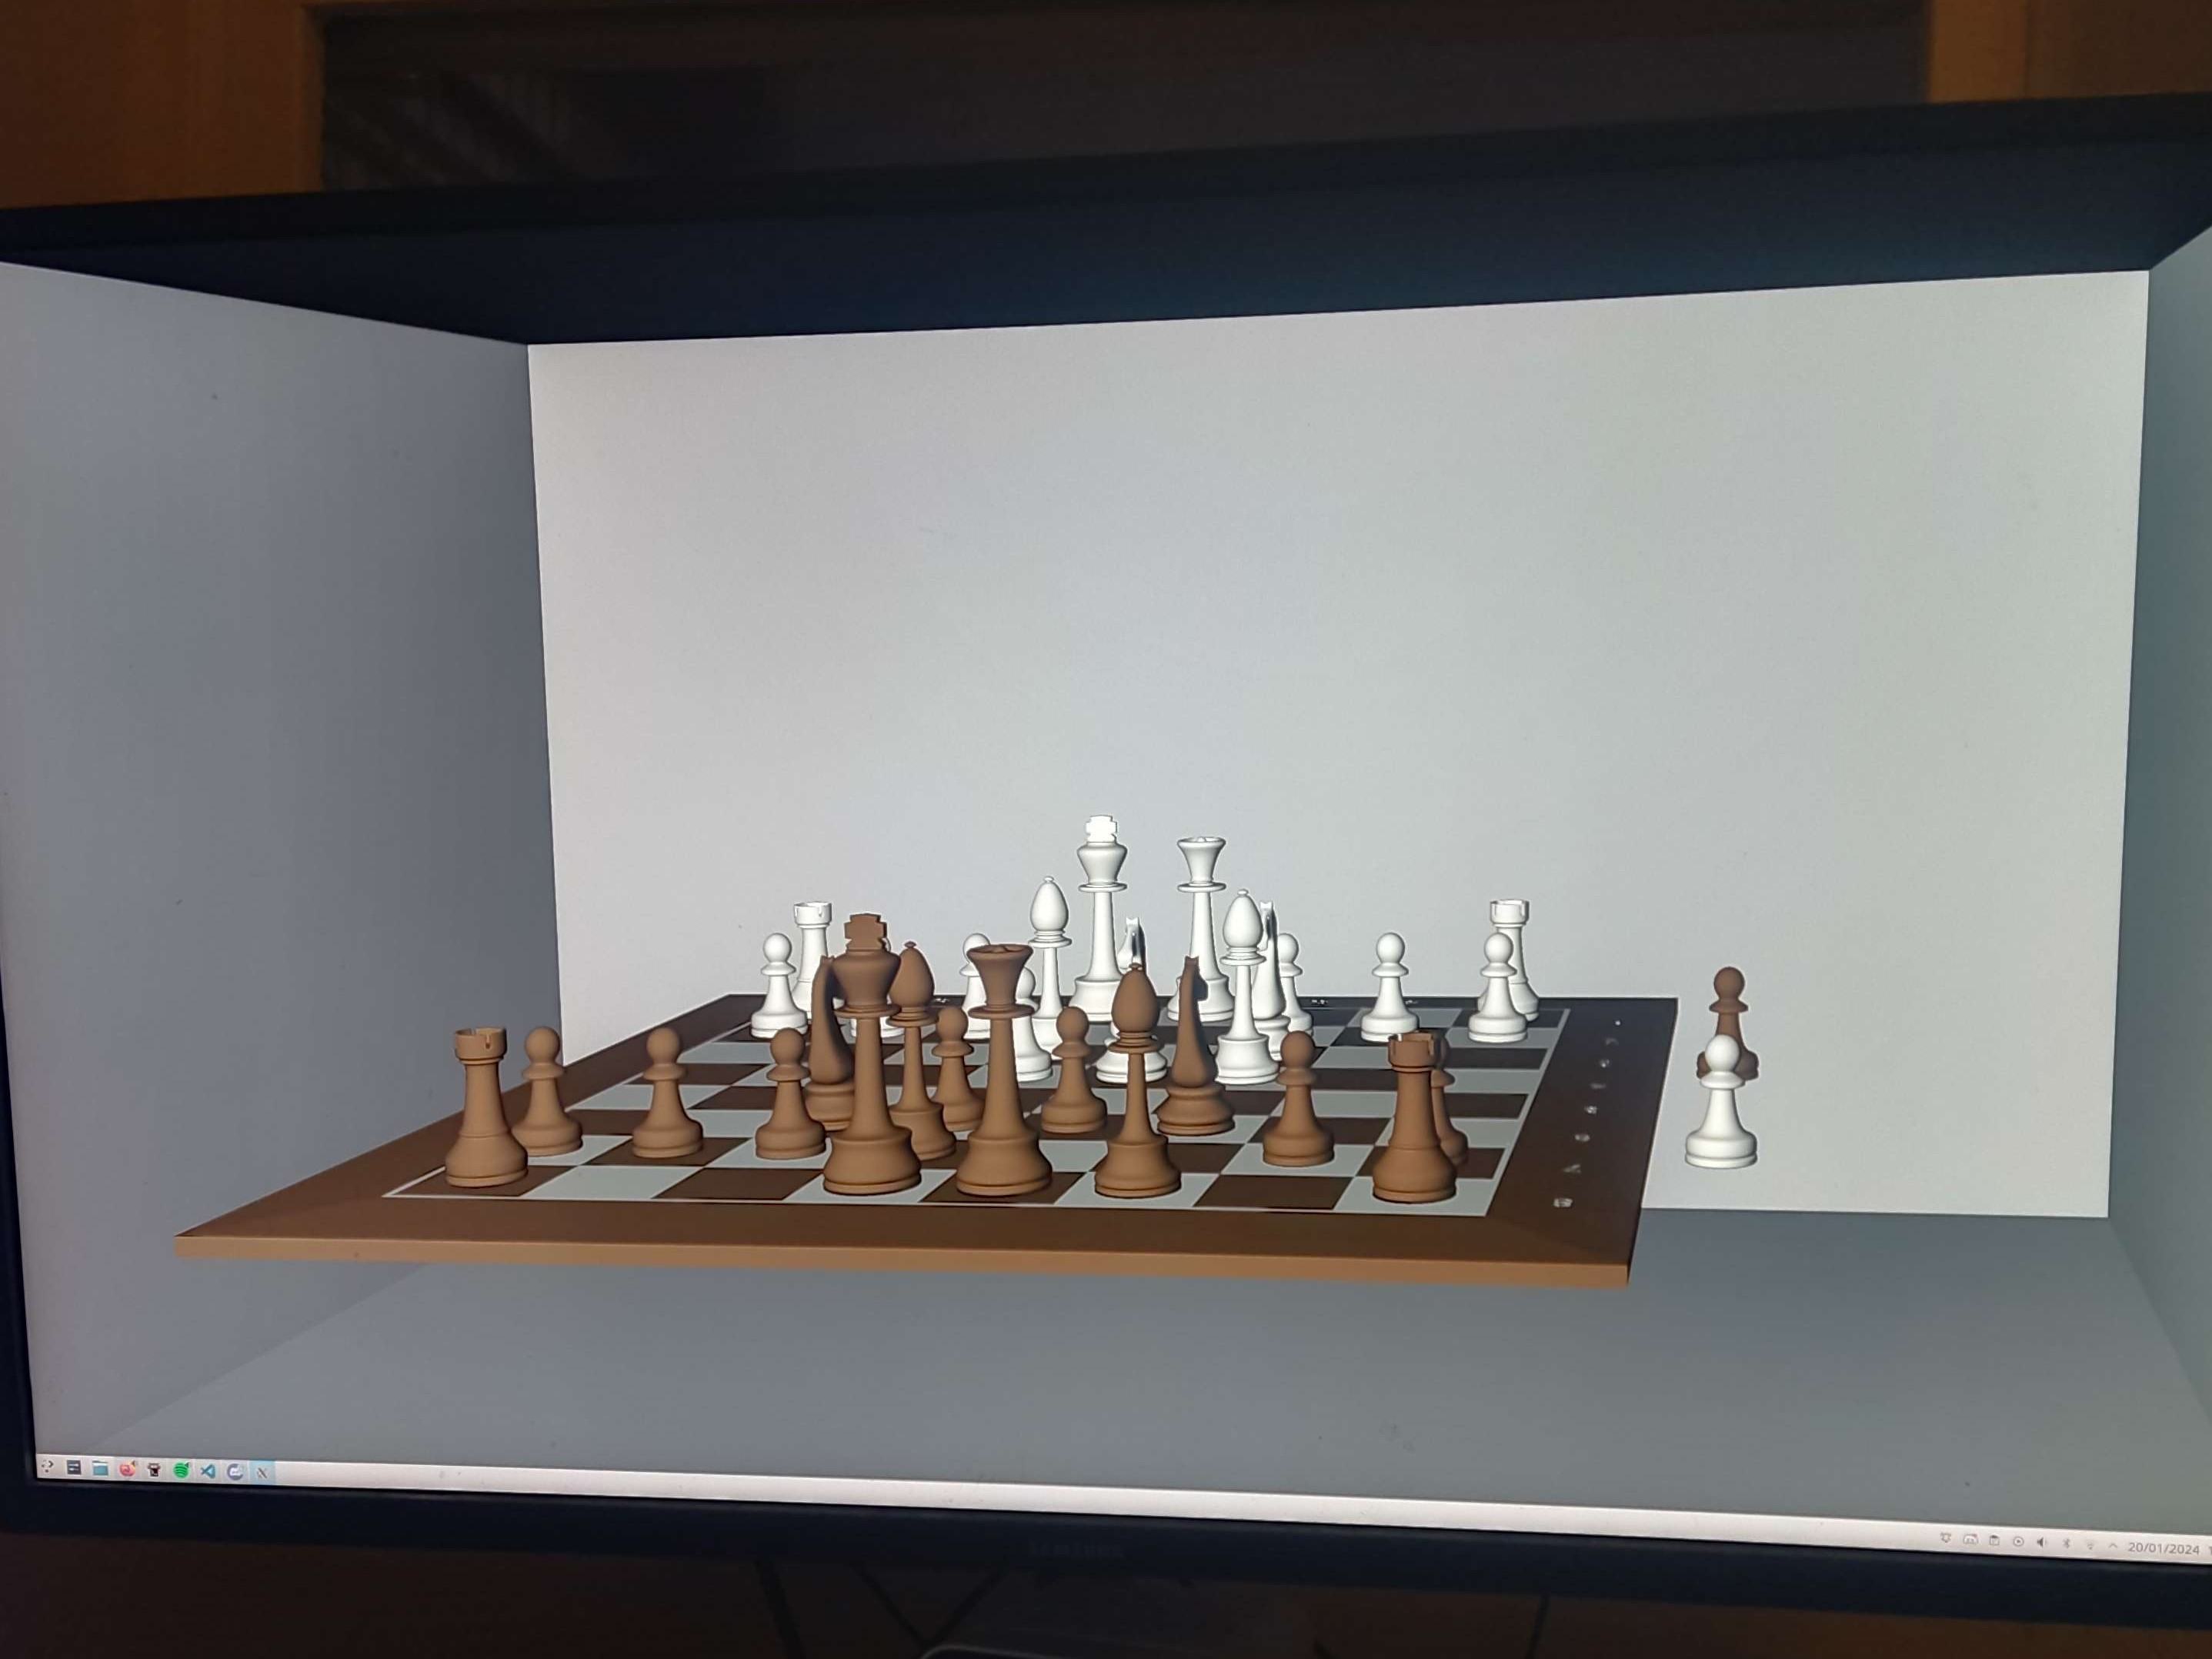
\includegraphics{./implementation/figures/perspective/right.jpg}
		}
	}
	\hfill
	\pictureBox[label={fig:left-view}]{Left Perspective}{
		\adjustbox{height=5.75cm, keepaspectratio}{
			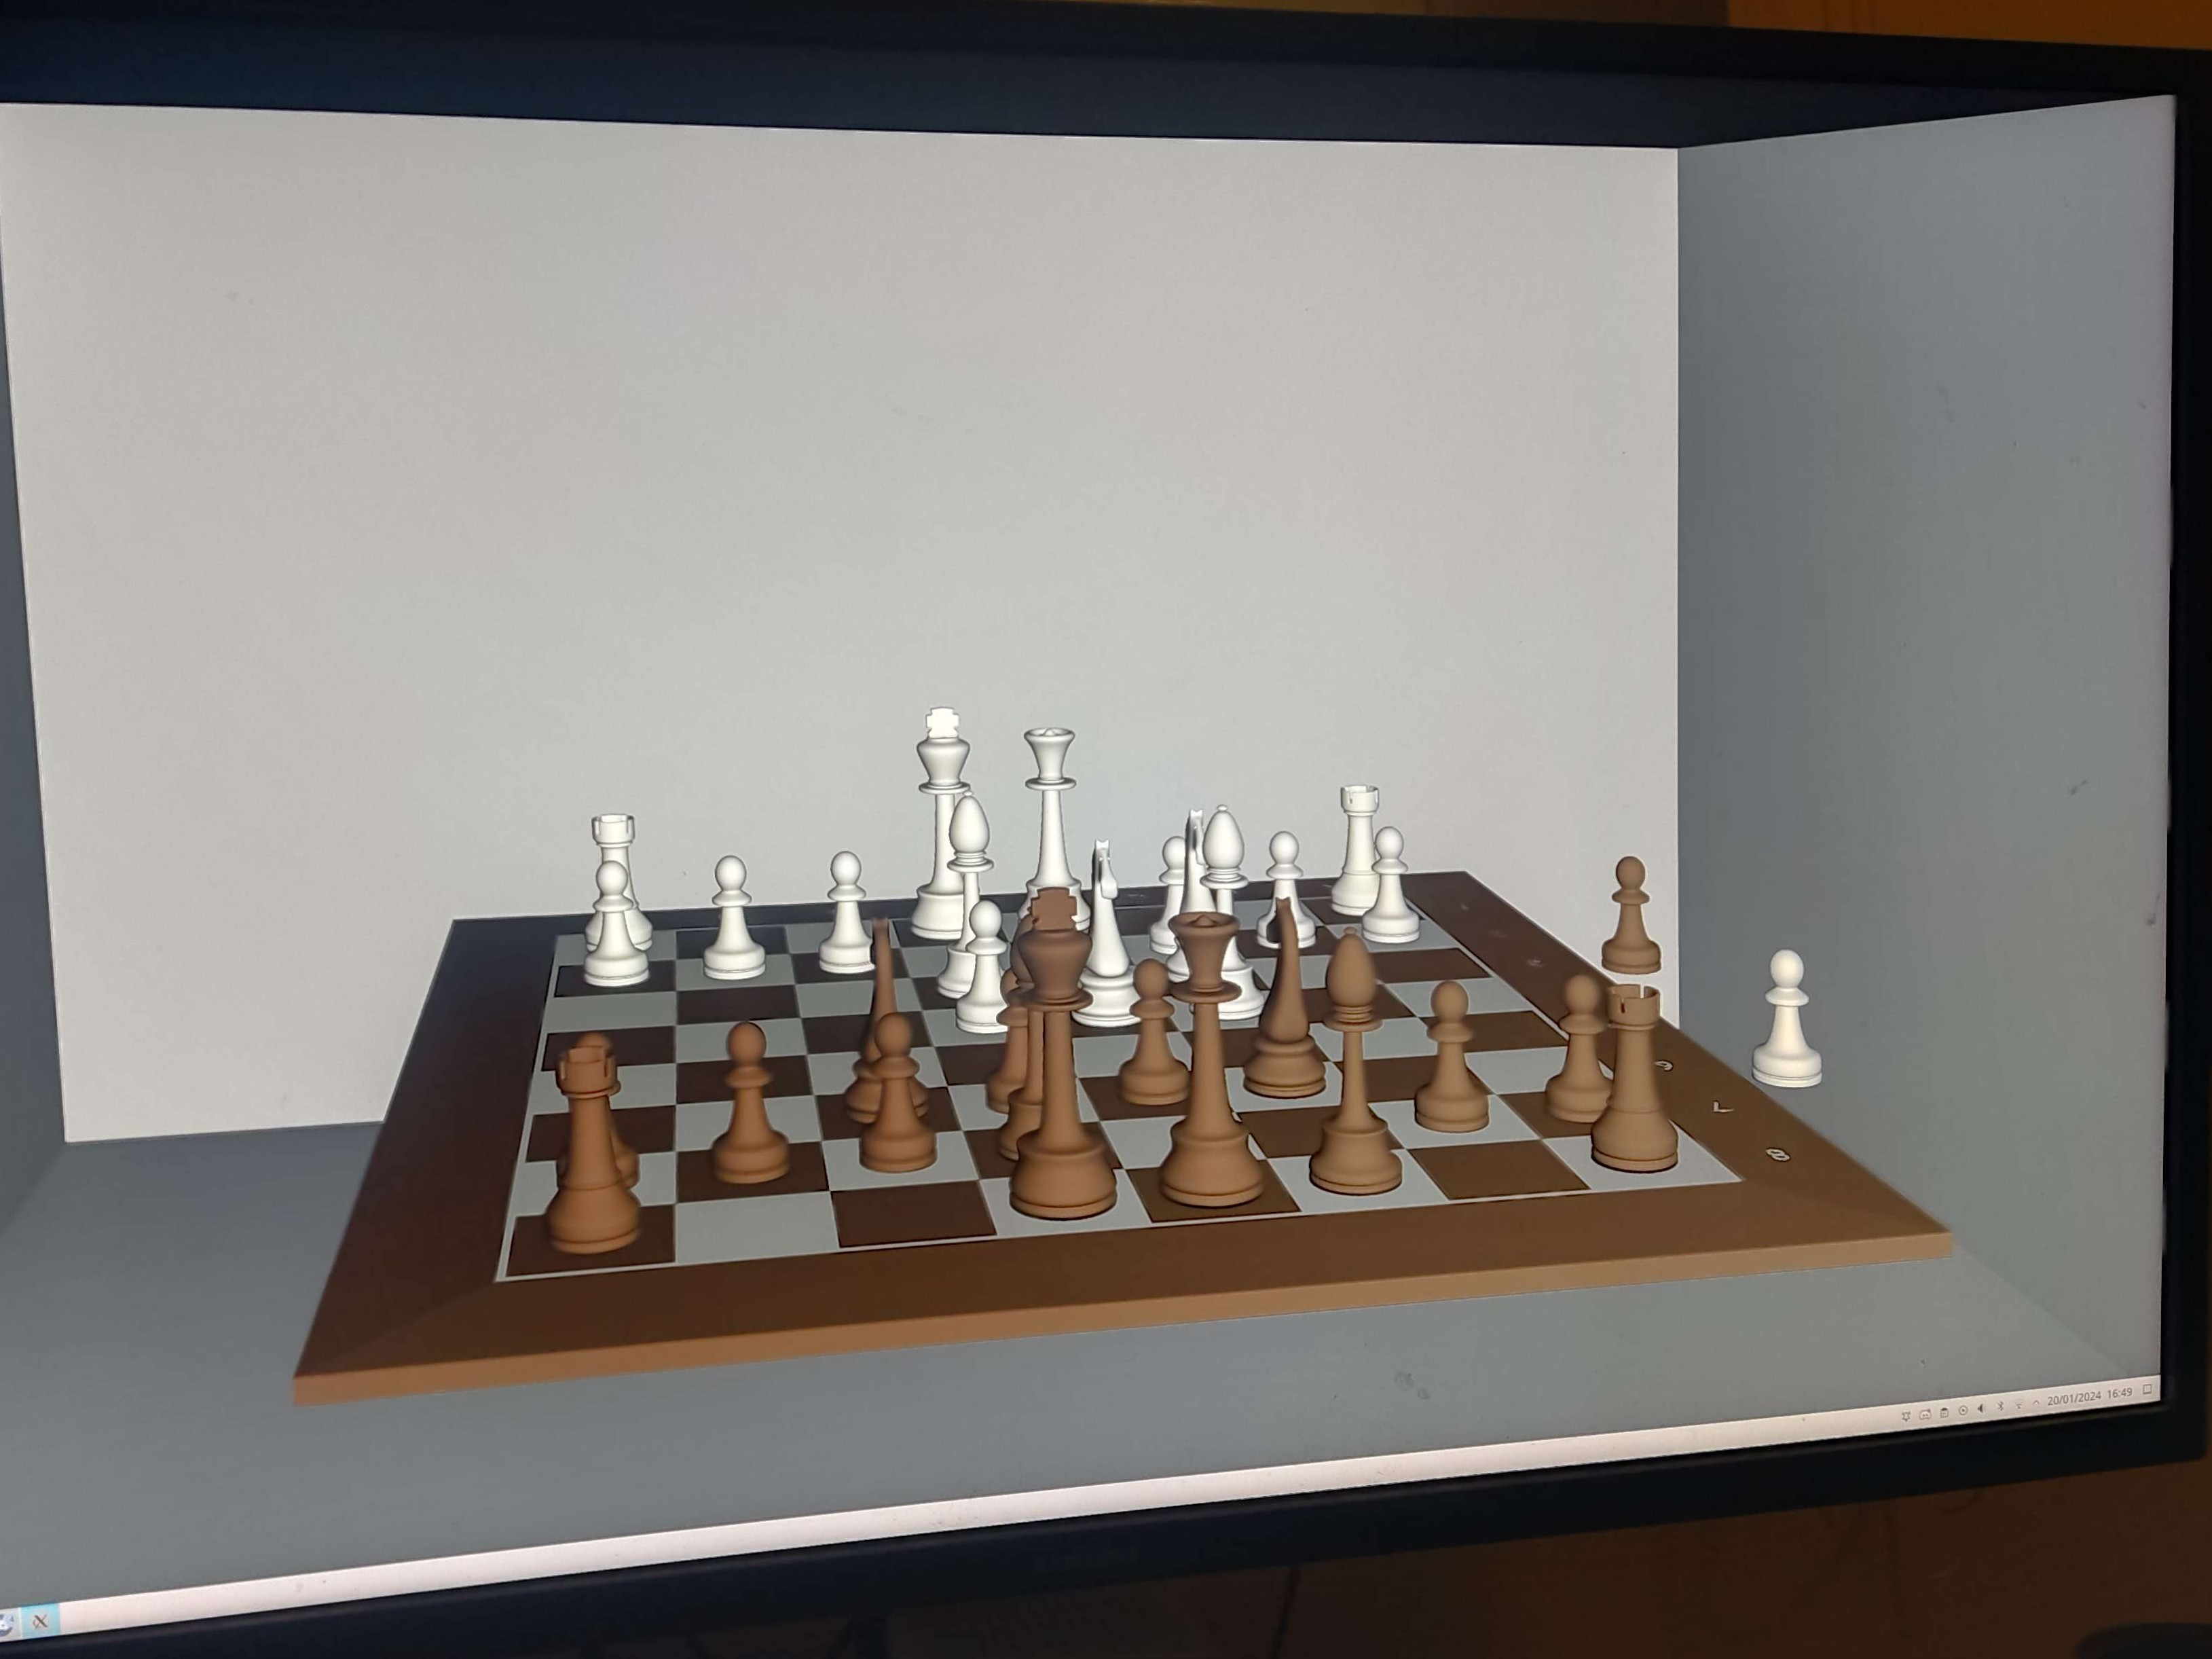
\includegraphics{./implementation/figures/perspective/left.jpg}
		}
	}
\end{invisBox}

\subsection{Object Loading}

Object loading support was added to the rendering system to facilitate the rendering of complex 3D models. We used the tinyobjloader library \cite{noauthor_tinyobjloadertinyobjloader_2024} to load \texttt{.obj} object files. We chose this library over alternatives like Assimp \cite{noauthor_assimpassimp_2024} due to its lightweight nature. We constructed our challenge for the user study by modifying primitives such as spheres, cylinders, and cubes loaded as \texttt{.obj} files using tinyobjloader to create an interactive task for the user.

\subsection{Lighting}

As shadows enhance the illusion of depth \cite{Kersten1997-xq}, we added a simple lighting model to the scene. We employed the Blinn-Phong \cite{10.1145/563858.563893} lighting model, which uses ambient, diffuse, and specular lighting. A comparison of the scene with and without lighting can be seen with the Erato Model \cite{McGuire2017Data} in Fig.~\ref{fig:erato} and Fig.~\ref{fig:erato-shadow}, respectively.

\begin{invisBox}
	\pictureBox[label={fig:erato}]{Erato}{
		\adjustbox{height=6.0cm, keepaspectratio}{
			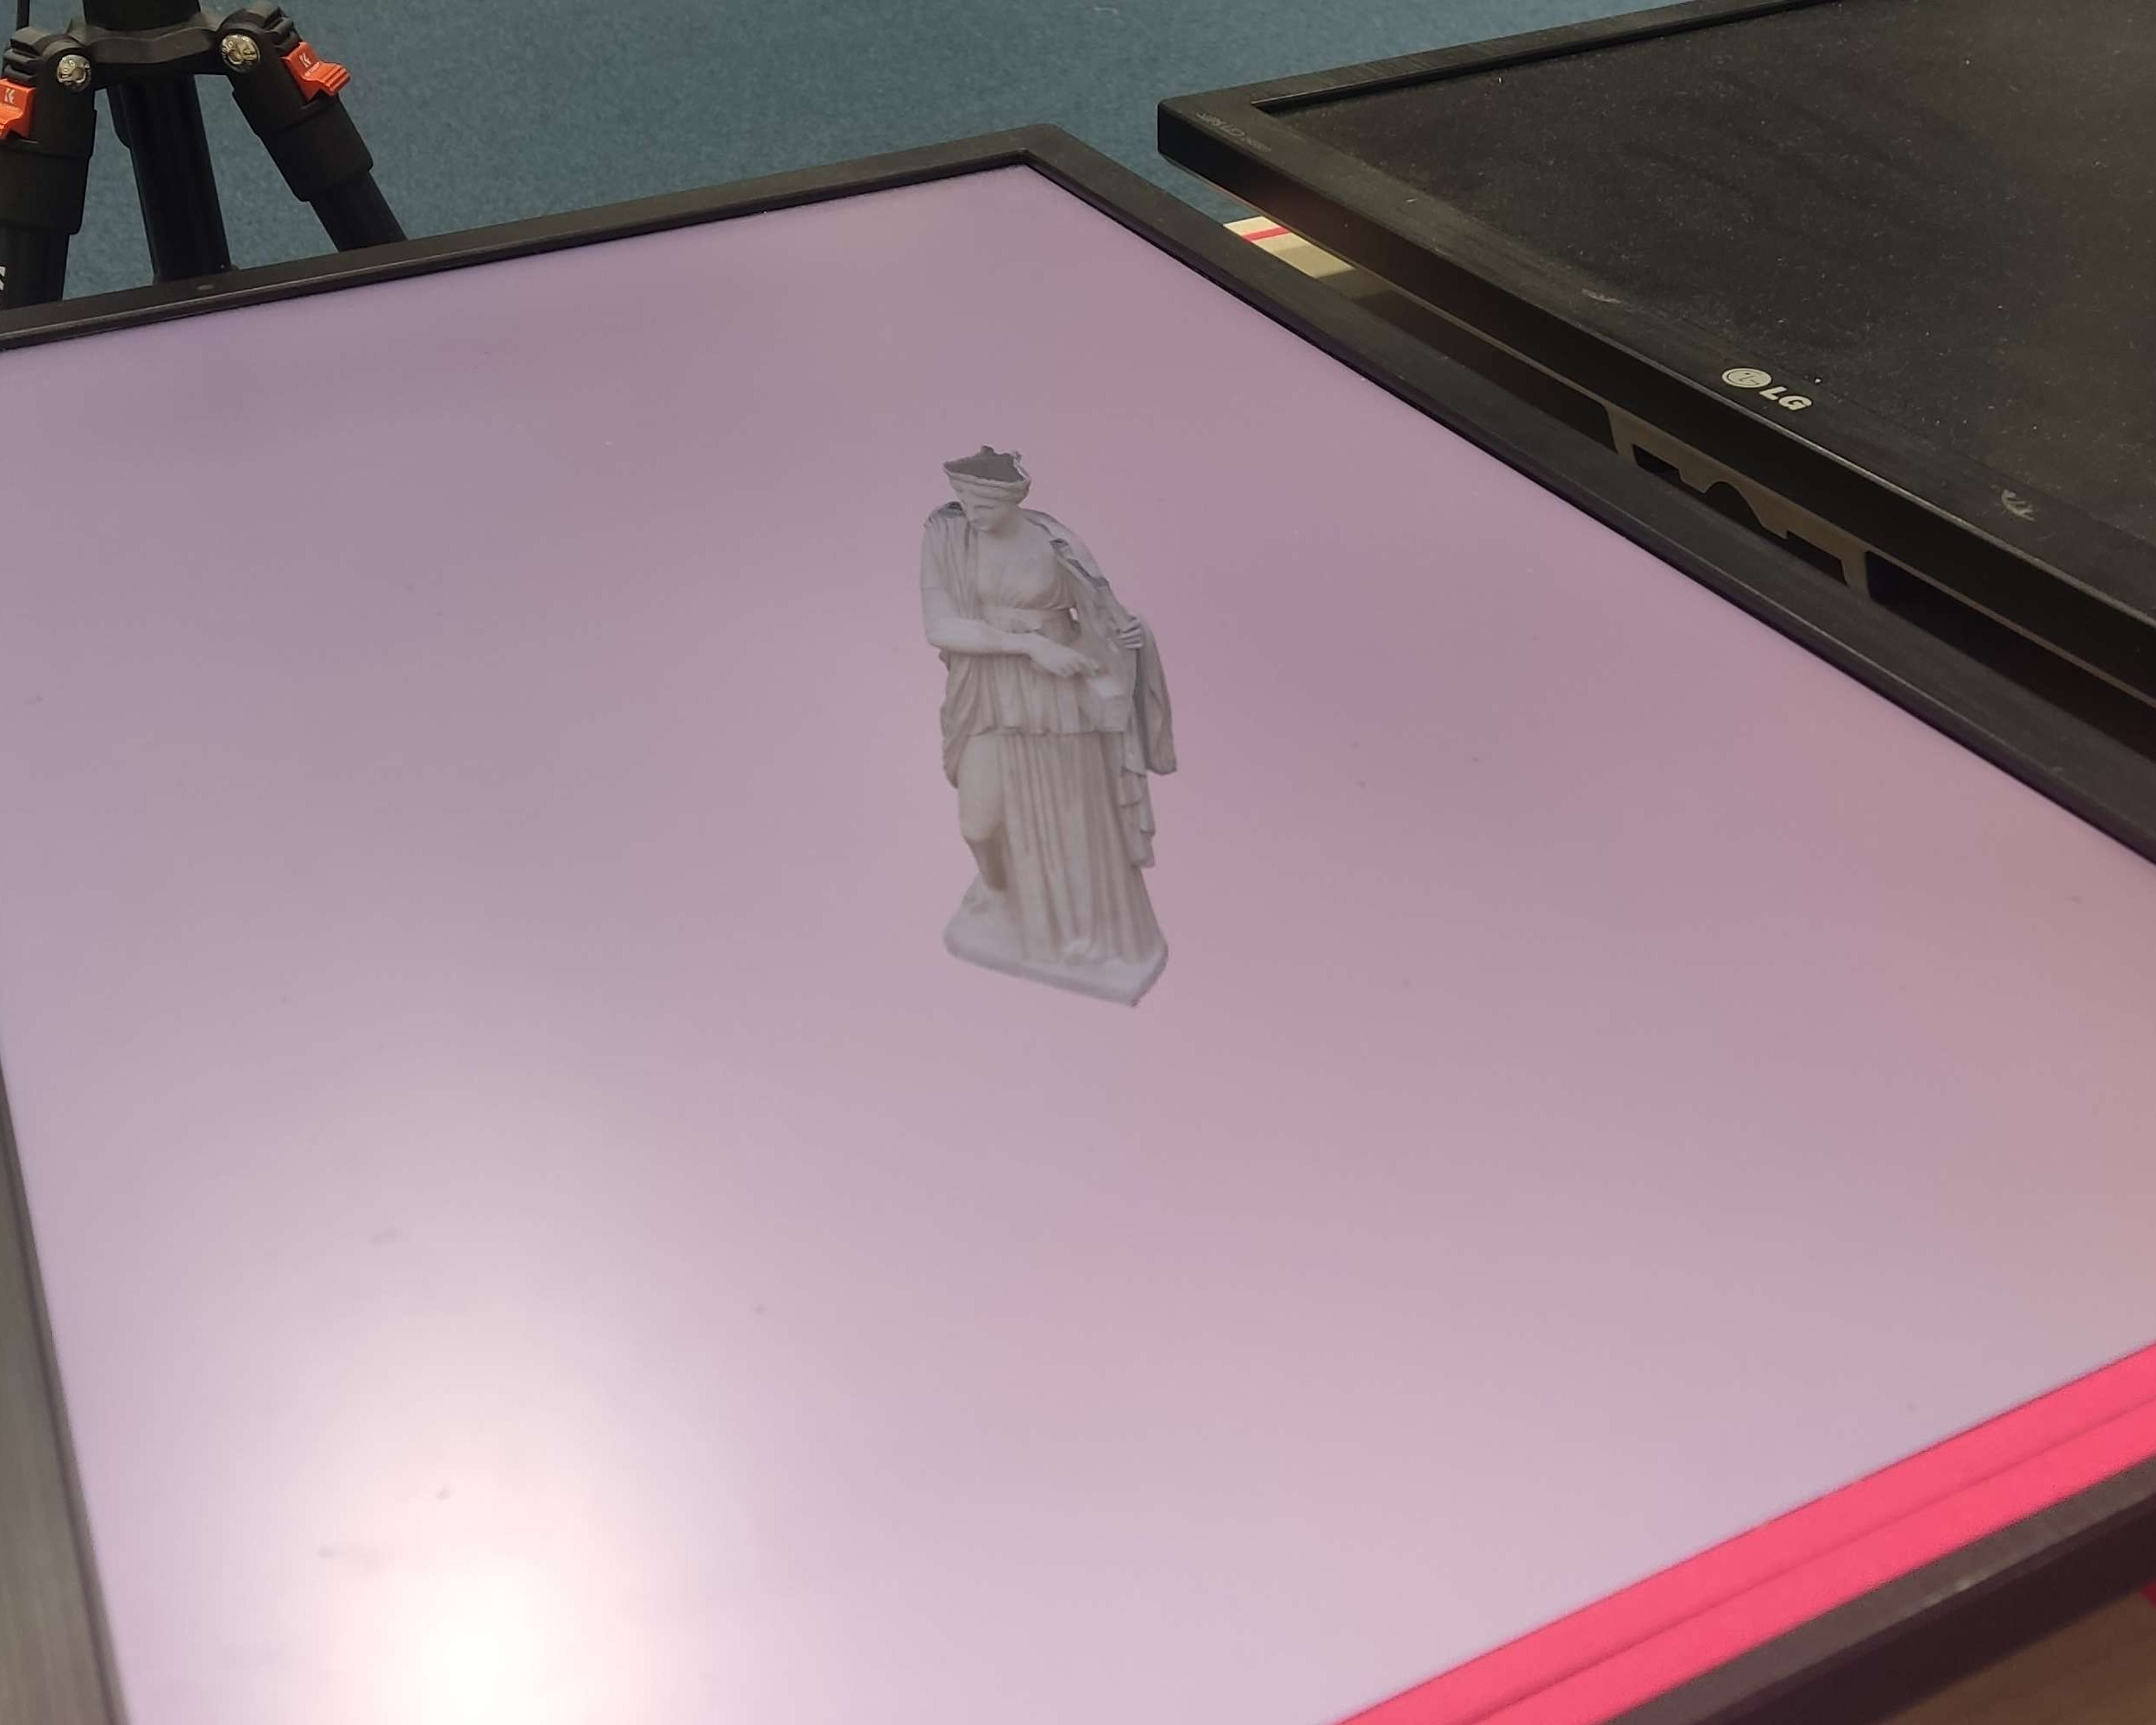
\includegraphics{./implementation/figures/perspective/erato.jpg}
		}
	}
	\hfill
	\pictureBox[label={fig:erato-shadow}]{Erato With Shadows}{
		\adjustbox{height=6.0cm, keepaspectratio}{
			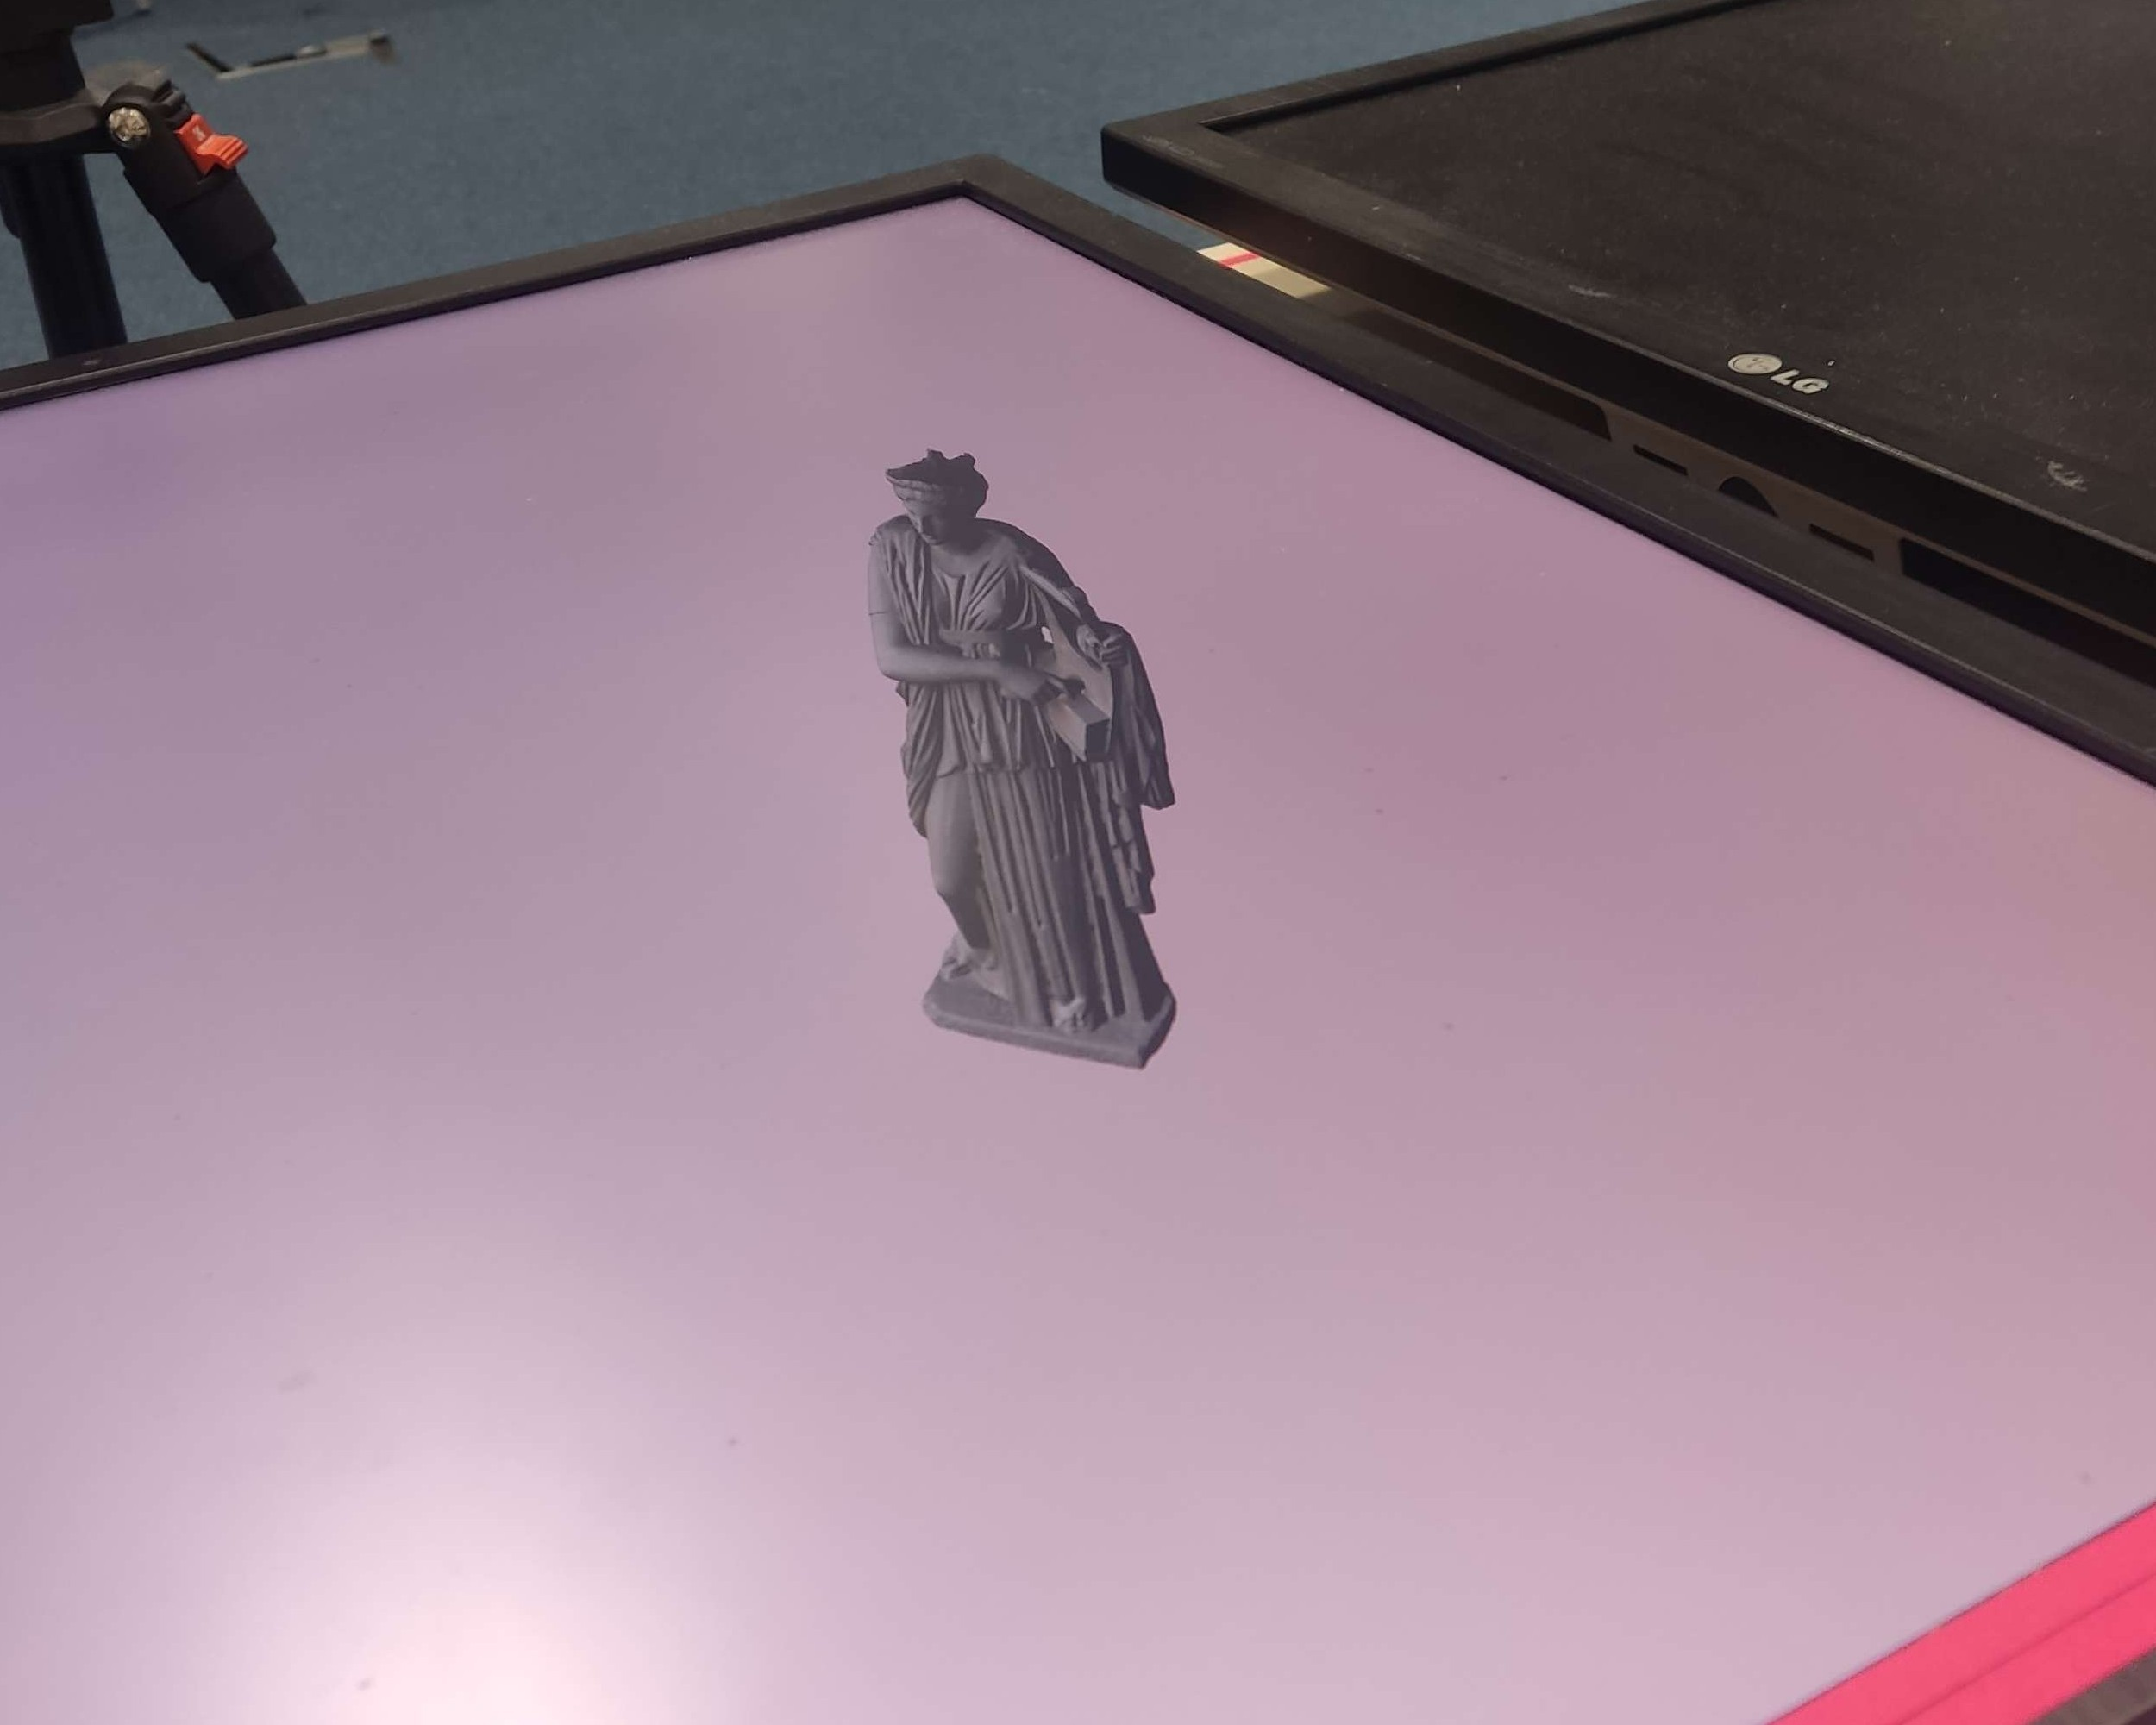
\includegraphics{./implementation/figures/perspective/erato_shadow.jpg}
		}
	}
\end{invisBox}

\label{sect:renderer}
\section{Tracking System}
\begin{enumerate}
	\item OpenCV for overall framework
	\item Dlib for face Tracking 
	\item Hand Tracking using MediaPipe
	\item Point cloud with tracked points.
\end{enumerate}
\label{sect:tracker}
\section{User Study}
\subsection{Introduction}
\begin{enumerate}
	\item The user study was conducted to evaluate the effectiveness of the system in improving the spatial reasoning skills of the participants.
\end{enumerate}

To validate the usefulness of our system we decided to conduct a Within-Subjects User Study. The user study was designed to show the capacity of the system for being used in research. The study was designed to test the effectiveness of users using volumetric displays under different conditions.

\subsection{Experimental Variables}
\begin{enumerate}
	\item Independent Variables:
	\begin{enumerate}
		\item 3D Perspective (On/Off)
		\item Interaction Offset (On/Off)
		\item So 4 conditions
	\end{enumerate}
	\item Dependent Variables:
	\begin{enumerate}
		\item Time taken to complete task
		\item Number of subtasks completed
		\item Eye and hand positions
	\end{enumerate}
	\item Control Variables:
	\begin{enumerate}
		\item The five tasks are the same in each condition.
		\item Position of participant
		\item Position of the tracking camera
		\item Position of the zone of interaction
		\item Size of the display. 
	\end{enumerate}
	\item Confounding Variables:
	\begin{enumerate}
		\item The participants may have different levels of experience with VR/Volumetric.
		\item Left-handed vs right-handed might make a difference for the tasks.
		\item Wearing glasses might make a difference for head tracking.
	\end{enumerate}
	\item 
\end{enumerate}

For this study we wanted to evaluate the difference in performance of participants in interacting with volumetric screens with their hands. 

Our two independent variables were: 
\begin{itemize}[itemsep=-0.25em]
	\item \textbf{3D Perspective}: (On/Off). This controls if the system is able to use the eye tracking system to create the illusion of a 3D volumetric display as can be seen in Fig~\todo.
	\item \textbf{Interaction Offset}: (On/Off). This controls if display is directly in front of the participant or if it is offset by a fixed amount as can be seen in Fig~\todo.
\end{itemize}
Giving us a total of 4 conditions to test.


The first condition we wanted to test was if there was any noticeable drop in performance when using the system in 2D (i.e with eye tracking disabled but still using hand tracking). The second condition was if there was a performance difference if participants "teleoperated" (controlled it with a fixed offset) the simulator vs using their hands directly. Combining these two conditions gives us the four conditions we tested as can be seen in Fig~\ref{fig:study-conditions}. 

\subsection{Tasks}
\begin{enumerate}
	\item Trace out points like a buzzwire game. 
	\item Draw Diagram of how the task works
	\item Draw Isometric view of the tasks
	\item Tasks are designed to be annoying if not in 3D.
	\item Timeout of 1 minute.
\end{enumerate}

In each of the 4 conditions the participant must complete the same 5 tasks. The tasks are designed to be simple but more difficult to complete if not in 3D. To complete a task a participant must trace the path between the points with their index and middle finger in the order the simulator presents to them. A green point is completed and an orange point represents the next point ot be completed as can be seen in Fig~\todo. \\ 

The participants have a timeout of 1 minute to complete the task. If they do not complete the task in the time limit, the task is marked as incomplete. The time each point is completed is recorded as well as the position of the hand and eye throughout the minute. The 5 different tasks are shown in Fig~\todo.

\subsection{Study Implementation}
\begin{enumerate}
	\item We run the study from a python based CLI (Click).
	\item We compile the simulator as a shared library and call it from the python CLI using a C-FFI.
	\item We receive the results and logs from python in json format and store them in a mongoDB database.
	\item This data is then used to generate the results.
\end{enumerate}

\subsection{Participants}
\begin{enumerate}
	\item We record age, gender, if they are left or right handed, and if they have any experience with VR, and if they wear glasses.
	\item The participants were given a random order of the four conditions.
	\item They complete the 5 tasks in each
	\item Fill out survey about each condition.
	\item Fill out survey about the system as a whole at the end.
	\item Ran the study in Huxley building.
\end{enumerate}

\subsection{Study Results}
\begin{enumerate}
	\item Use ANOVA test?
	\item ????
\end{enumerate}

\label{sect:userstudy}

% %%%%%%%%%%%%%%%%%%%%%%%%%%%%%%%%%%%%
\chapter{Evaluation}
\section{Simulator Evaluation}

To ensure that our system meets the quality standards necessary for research purposes and accurately simulates a volumetric display, we conducted a comprehensive evaluation using various metrics.

\subsection{Overall System}

The initial step in our evaluation process involved assessing the performance of the system.

\textcolor{red}{TODO don't edit this part}
\begin{enumerate}
    \item Benchmark the system, including GPU and CPU usage using tools such as HTOP and NVIDA-SMI.
\end{enumerate}

\subsection{Tracking System: Frame Rate, Latency, and Timings}

To gain deeper insights into the performance and quality of the tracking system, we conducted several tests. The primary focus was on the inter-update gap, defined as the time interval between consecutive tracker frames being sent to the renderer.

\begin{figureBox}[label={fig:framerate-overall}, width=1.0\linewidth]{Tracker Inter-Update Gap (over 5 mins)}
    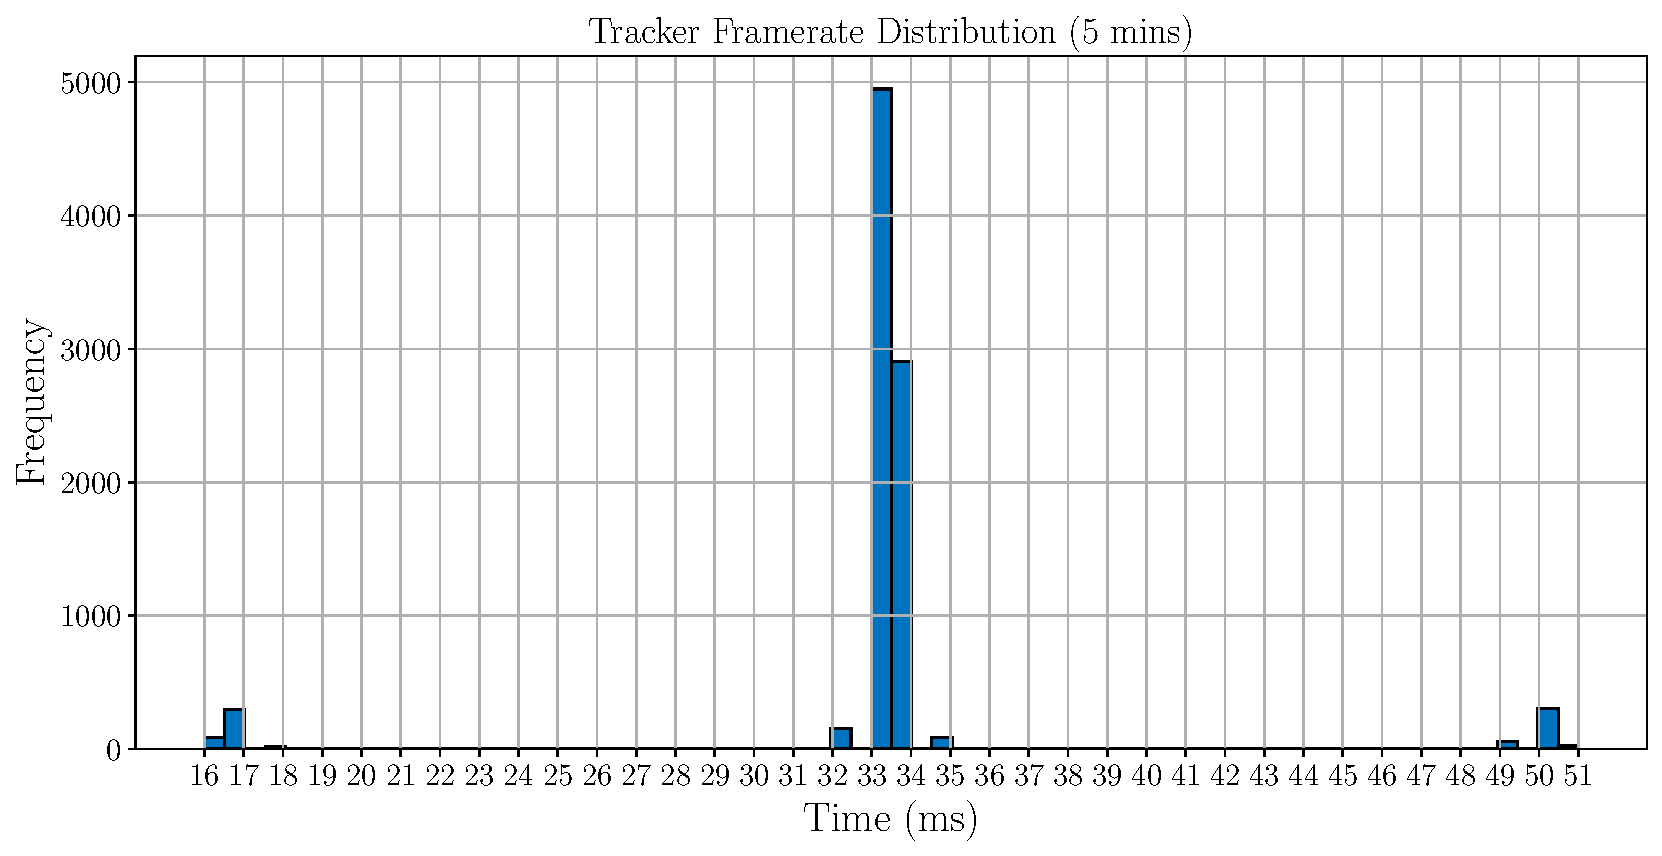
\includegraphics[width = 1.0\linewidth]{./evaluation/figures/framerate-overall.pdf}
\end{figureBox}

As depicted in Figure \ref{fig:framerate-overall}, the system's frame rate remained relatively consistent, with 90.83\% of frames maintaining a latency between 30 and 35 ms. A peculiar observation was the cluster of latencies at 16-18 ms (4.46\%) and 49-51 ms (4.39\%). This anomaly is attributed to the frame rate of the renderer, as our system performs lazy conversion of 2D points to 3D only when necessary. Our renderer operates at 60 fps, constrained by our monitors, resulting in frame intervals approximating to 16.666 ms. Although our tracker functions at 30 fps (33.33 ms inter-update gap), there can be an inter-update gap of 16 ms if the tracker is delayed past the initial 33.33 ms, causing an additional delay of approximately 16.66 ms, resulting in a total gap of around 50 ms. However, during this waiting period, another frame is processed and ready for the next cycle, giving the appearance of a higher frame rate than 30 fps.

\subsubsection{Downscaling Benchmarks}

In exploring the impact of downscaling on performance, we determined that a single instance of downscaling sufficed to meet our performance requirements. Further downscaling did not yield significant performance benefits and adversely affected tracking quality. Figure \ref{fig:pydown} illustrates our findings, showing a noticeable performance improvement when reducing the resolution from the source $2048 \times 1536$ to $1024 \times 793$. Additional reductions in resolution did not provide further speed benefits, as the bottleneck was the 30 fps frame rate of the Kinect camera.

\begin{figureBox}[label={fig:pydown}, width=1.0\linewidth]{Comparing Inter-Update Gap By Resolutions (over 1 min)}
    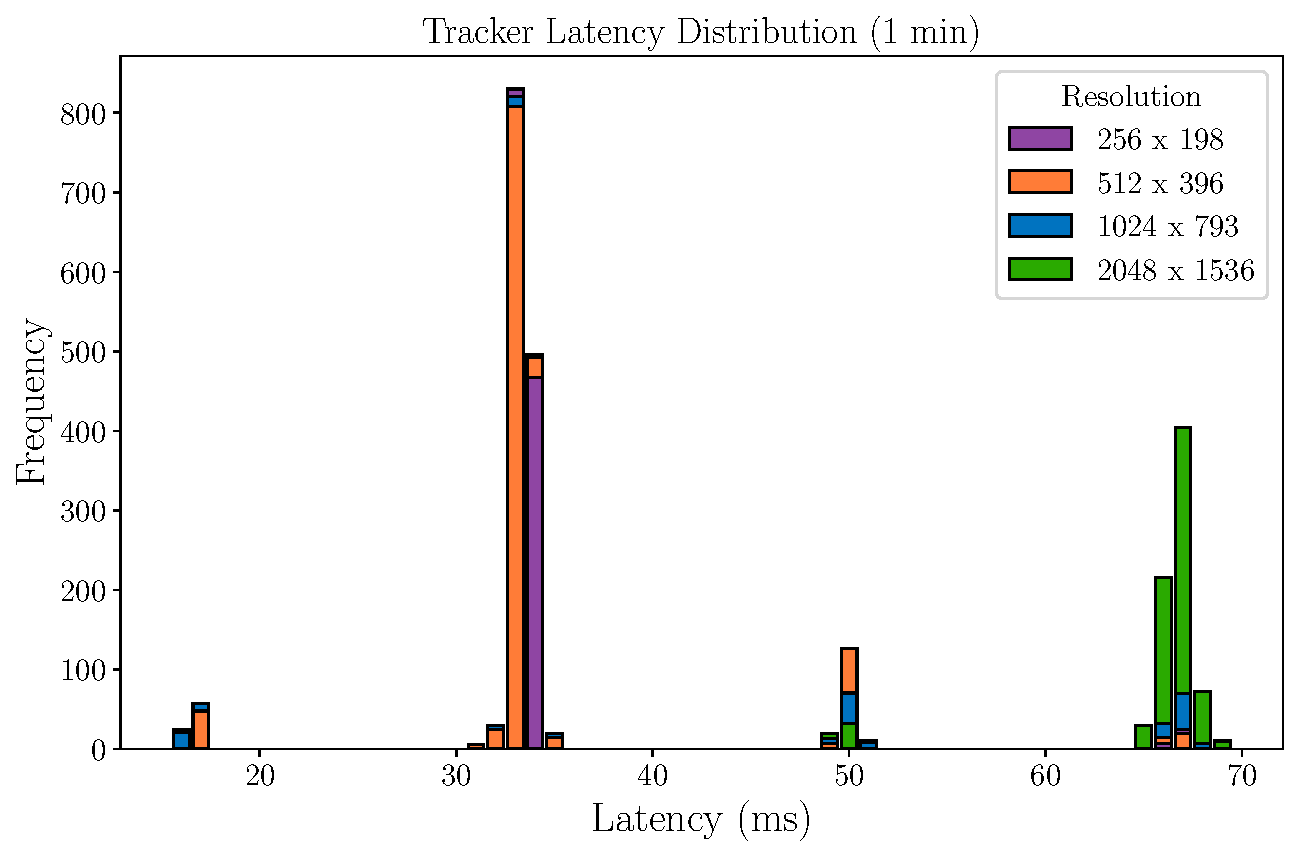
\includegraphics[width = 1.0\linewidth]{./evaluation/figures/pydown.pdf}
\end{figureBox}

\subsubsection{Timings by Subprocess}

Further investigation revealed that among the three concurrent threads (capturing from the Kinect camera, tracking hand and eye movements, and rendering with OpenGL), the primary bottleneck was waiting for the Kinect camera to complete the capture. Figure \ref{fig:process-times-distributions} highlights that expediting the tracking algorithm offered limited benefit due to this bottleneck.

\begin{figureBox}[label={fig:process-times-distributions}, width=1.0\linewidth]{Comparing Thread Competition Times}
    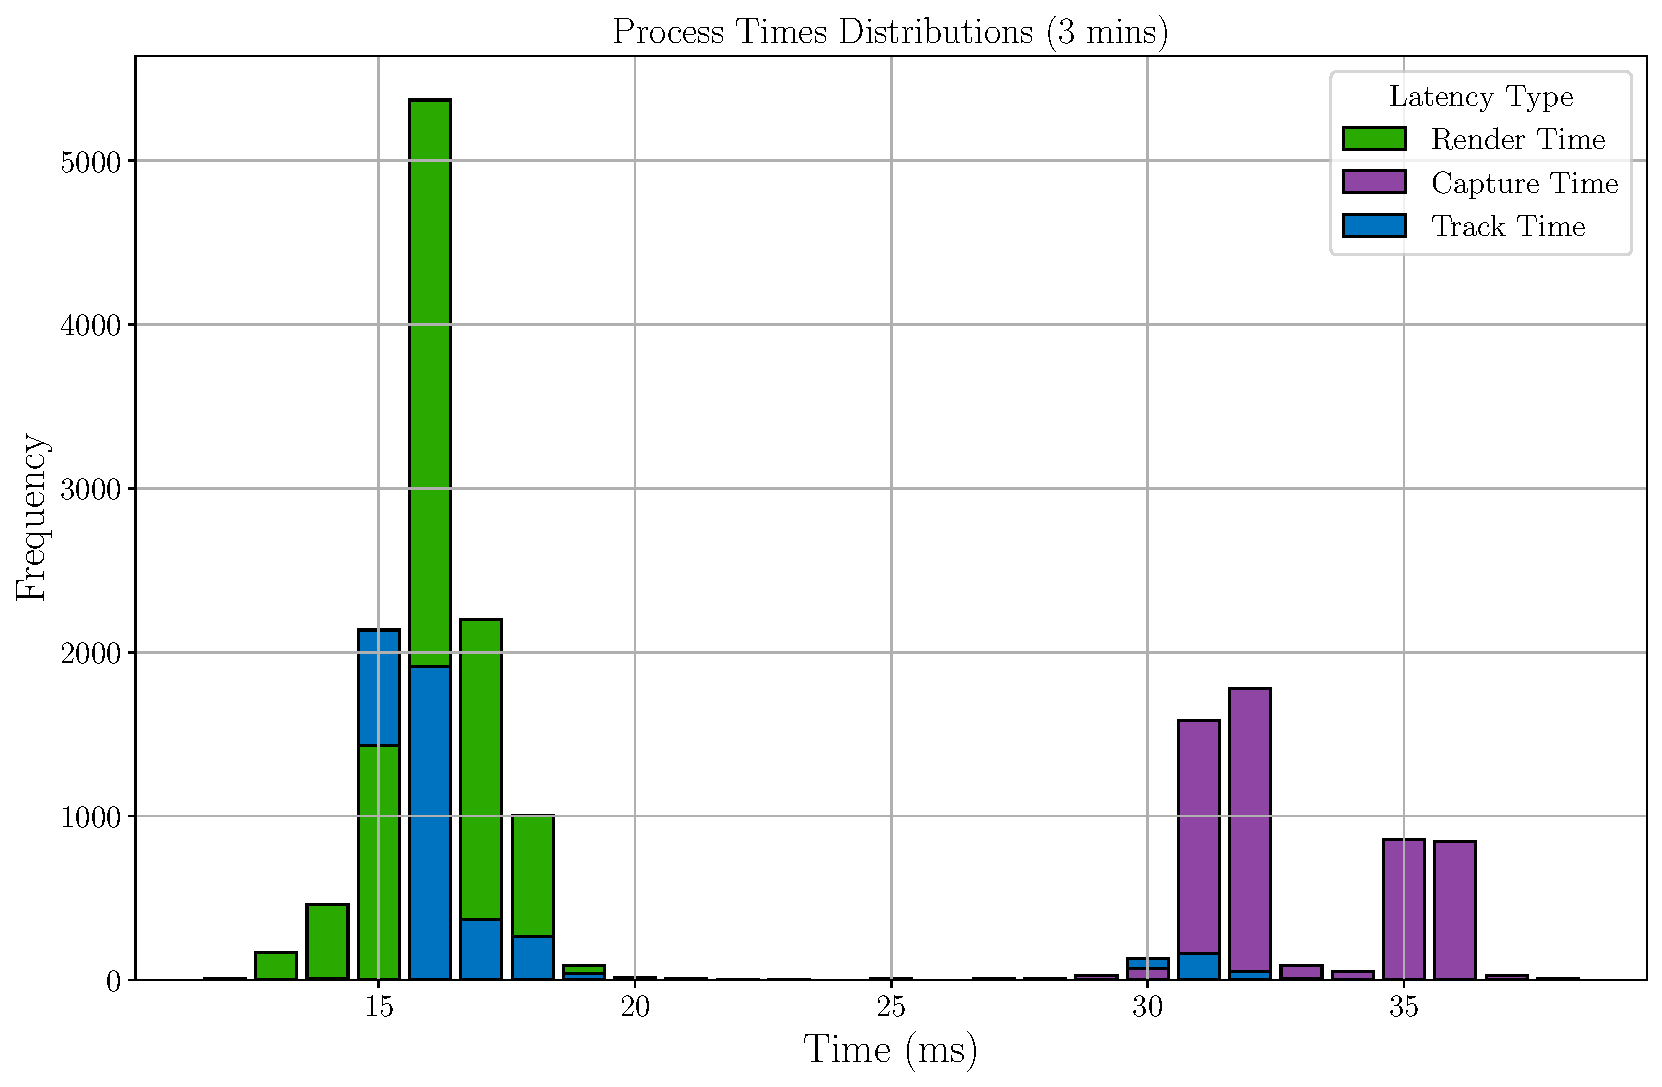
\includegraphics[width = 1.0\linewidth]{./evaluation/figures/process-times-distributions.pdf}
\end{figureBox}

\subsubsection{Latency from Camera to Eye}

Although precise latency statistics for the Azure Kinect from capture to device are unavailable, estimates suggest a latency of around 90 ms \cite{gholami2023autodepthnet}. Considering the time required for OpenGL primitives to display images on the screen, which ranges from 10 to 30 ms depending on the display \cite{https://doi.org/10.1002/jsid.1104} \cite{noauthor_latency_nodate}, and combining this with our system's processing time of less than 30 ms, we estimate the total system latency to be approximately 150 ms. \\

When compared to state-of-the-art systems in similar fields such as VR, our system exhibits higher latency, as shown in Table \ref{tab:photon-to-photon-latency}.

\begin{table}[h!]
    \centering
    \caption{Our Photo-to-Photon Latency Vs Common VR Systems reported by OptoFidelity \cite{noauthor_apple_2024}}
    \label{tab:photon-to-photon-latency}
    \begin{tabular}{lS[table-format=1.2e+2]S[table-format=4.0]S[table-format=2.6]S[table-format=1.6]}
        \toprule
        \textbf{System} & \textbf{Latency (ms)}\\
        \midrule
        \texttt{Volumetric Simulator (\textbf{Ours})} & ~150ms \\
		\texttt{HTC VIVA XR Elite} & ~40ms\\
		\texttt{Meta Quest 3} & ~39ms \\
		\texttt{Meta Quest Pro} & ~38ms \\
        \texttt{Apple Vision Pro} & ~11ms  \\
        \bottomrule
    \end{tabular}
\end{table}

It is challenging to directly compare our system with other similar systems, such as the Multi-person Fish-Tank Virtual Reality Display \cite{10.1145/3281505.3281540} \cite{10.1145/169059.169066} or systems used in 3D Display Simulation Using Head-Tracking with Microsoft Kinect \cite{Zabarauskas2012}, as they do not report their latencies. However, given that both systems utilize Kinect cameras, which are a significant source of latency, we can infer that our system likely has comparable latency to these systems.

\subsection{Tracking System: Accuracy}

Evaluating the accuracy of our tracking system is crucial to ensure its reliability and effectiveness.

\subsubsection{Effective Range}

The first aspect of the evaluation focused on the effective tracking range of our system. We placed a participant in a fixed position on a chair and instructed them to slowly wave their hand and move their head. An example of the test setup is shown in Figure~\ref{fig:distance-setup}. We conducted tests at various distances, recording the percentage of successful captures that detected a face or hand at 30-second intervals. The resolution of the color image used for this test was $1024 \times 793$.

\begin{invisBox}
    \pictureBox[label={fig:distance-setup}]{Setup for Distance Testing}{
        \adjustbox{height=5cm, keepaspectratio}{
            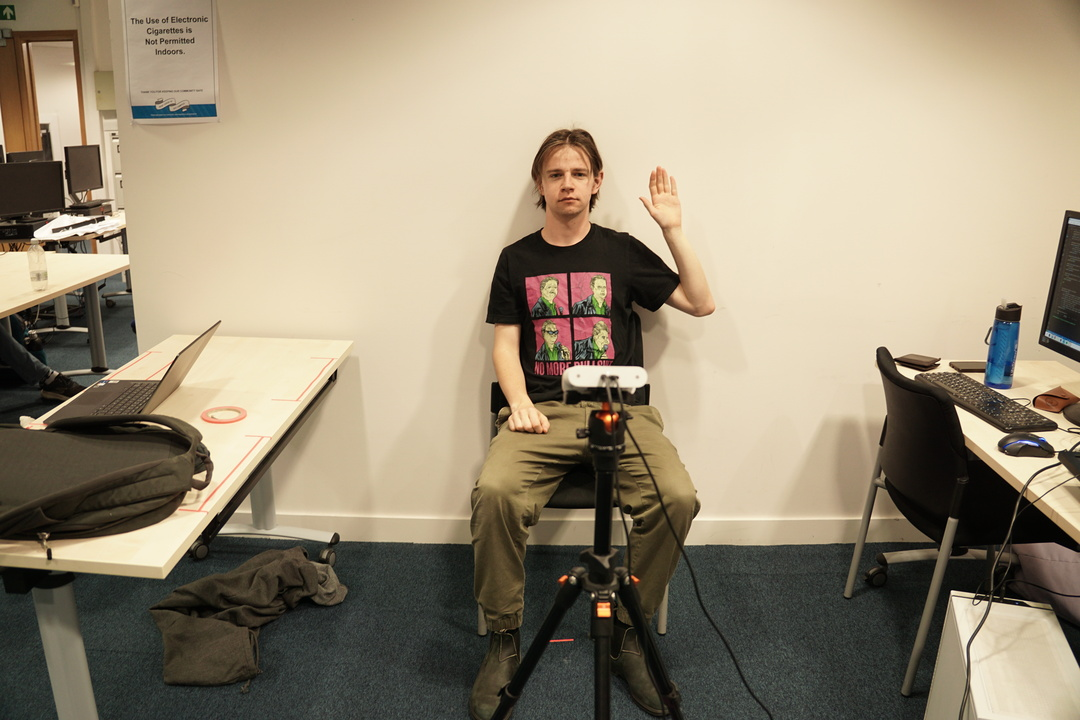
\includegraphics{./evaluation/figures/distance_setup.jpg}
        }
    }
    \hfill
    \pictureBox[label={fig:track-distance}]{Success Rate at Varying Distances}{
        \adjustbox{height=5.0cm, keepaspectratio}{
            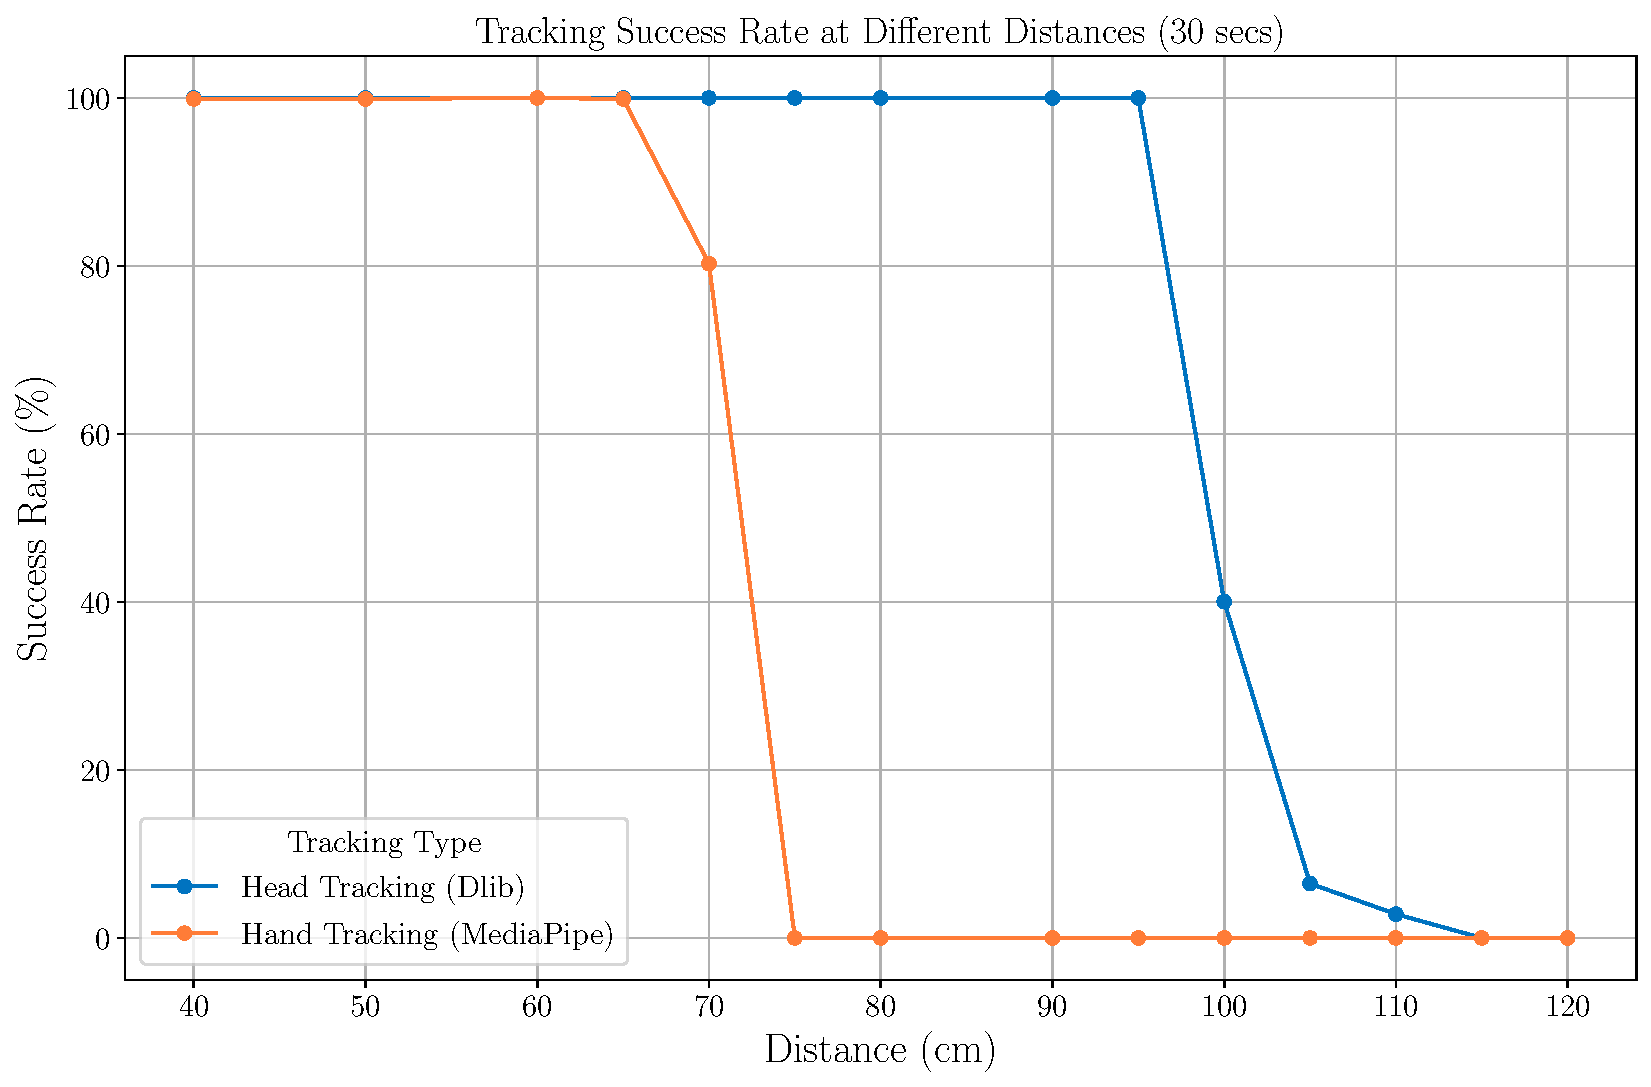
\includegraphics{./evaluation/figures/tracking-success-rate.pdf}
        }
    }
\end{invisBox}

As illustrated in Figure~\ref{fig:track-distance}, the success rate for MediaPipe's hand tracking model rapidly decreases after 1 meter, ultimately failing 100\% of the time at greater distances. This is likely due to the dataset it was trained on and its primary design for tracking hands using a mobile phone camera \cite{dlib09}. \\

Dlib's head tracking model performed better, with effective tracking up to approximately 1.5 meters. The decline in performance beyond this distance is similarly attributed to the nature of its training data. These findings were considered in the design of our user study, where the camera was positioned to keep the user's hand within 30-70 cm and the head within 1 meter from the camera.

\subsubsection{Head Tracking}

The effectiveness of the head tracking system is another critical aspect, particularly the range of head positions at which tracking is possible. Specifically, we were interested in the angle at which the model fails to detect a face. We set up a straightforward experiment, shown in Figure~\ref{fig:angle-setup}, to measure the head angles at which the tracking system ceases to function. Participants were seated on a swivel chair and asked to keep their body still while rotating their head. We noted the position of the midpoint of their feet when tracking failed, and used basic trigonometry to estimate the head angle.

\begin{figureBox}[label={fig:angle-setup}, width=1.0\linewidth]{Angle Setup}
    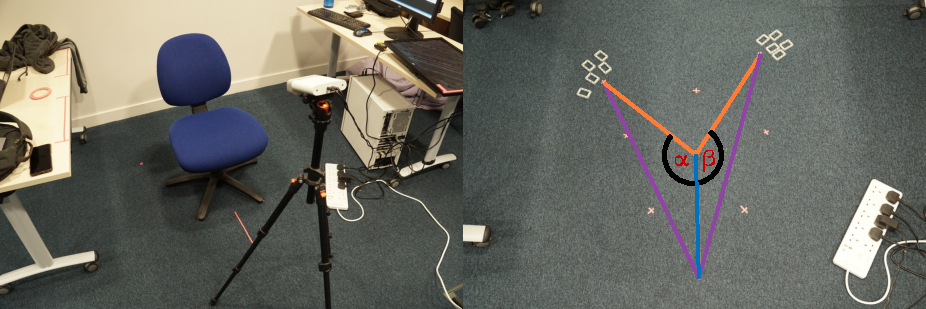
\includegraphics[width = 1.0\linewidth]{./evaluation/figures/angle-setup.pdf}
\end{figureBox}

This test involved five participants, with results presented in Figure~\ref{fig:head-angle}. Although the technique was somewhat rudimentary and thus not highly precise, the angle at which head tracking typically failed ranged between $120^{\circ}$ and $150^{\circ}$. This result may seem counterintuitive, as at these angles, the participant is facing away from the camera. However, the face tracking model first detects a face and then maps landmarks to it, even when the face is not directly visible.

\begin{invisBox}
    \pictureBox[label={fig:head-angle}]{Angle of Failure for Head Tracking}{
        \adjustbox{height=6cm, keepaspectratio}{
            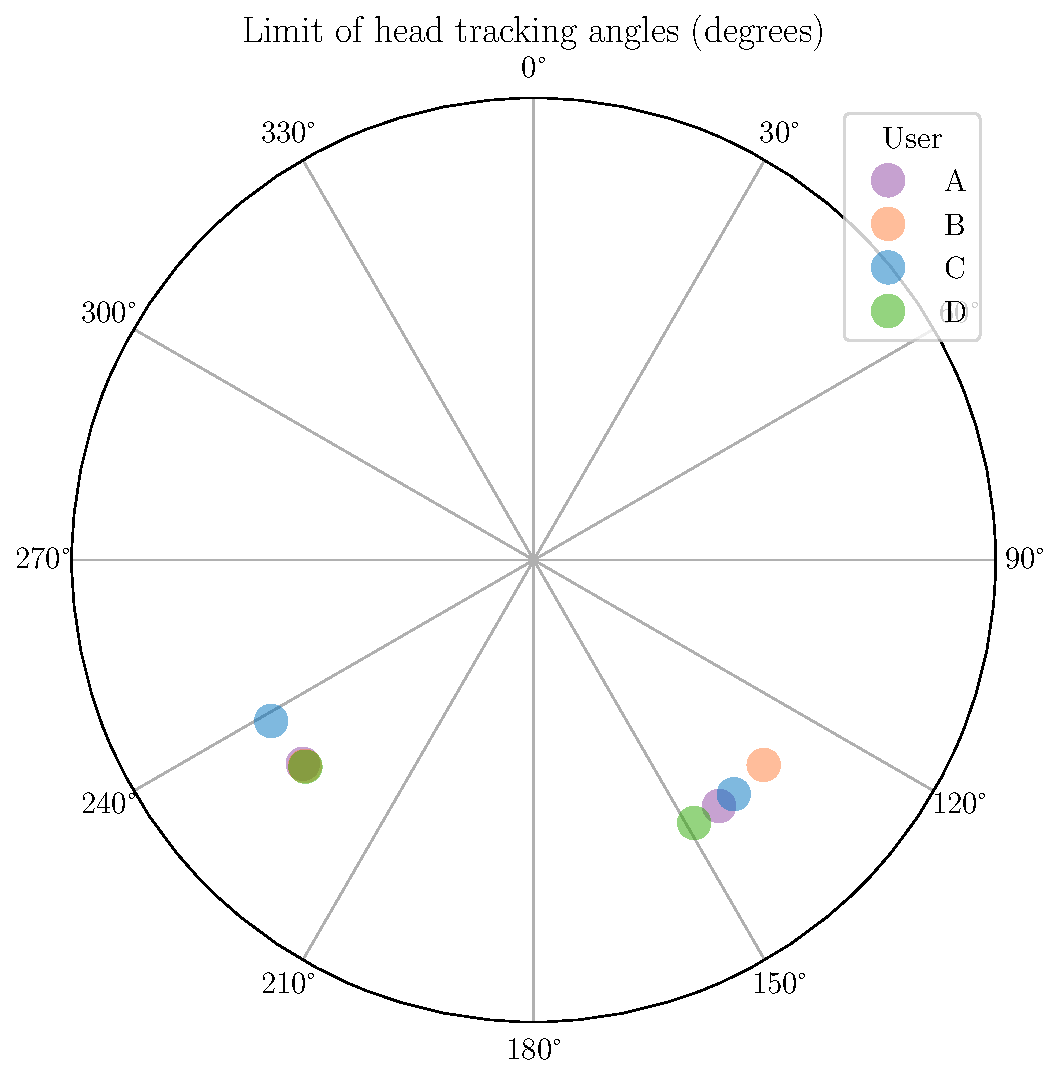
\includegraphics{./evaluation/figures/user-angles.pdf}
        }
    }
    \hfill
    \pictureBox[label={fig:incorrect-head-track}]{Incorrect Head Tracking}{
        \adjustbox{height=6.5cm, keepaspectratio}{
            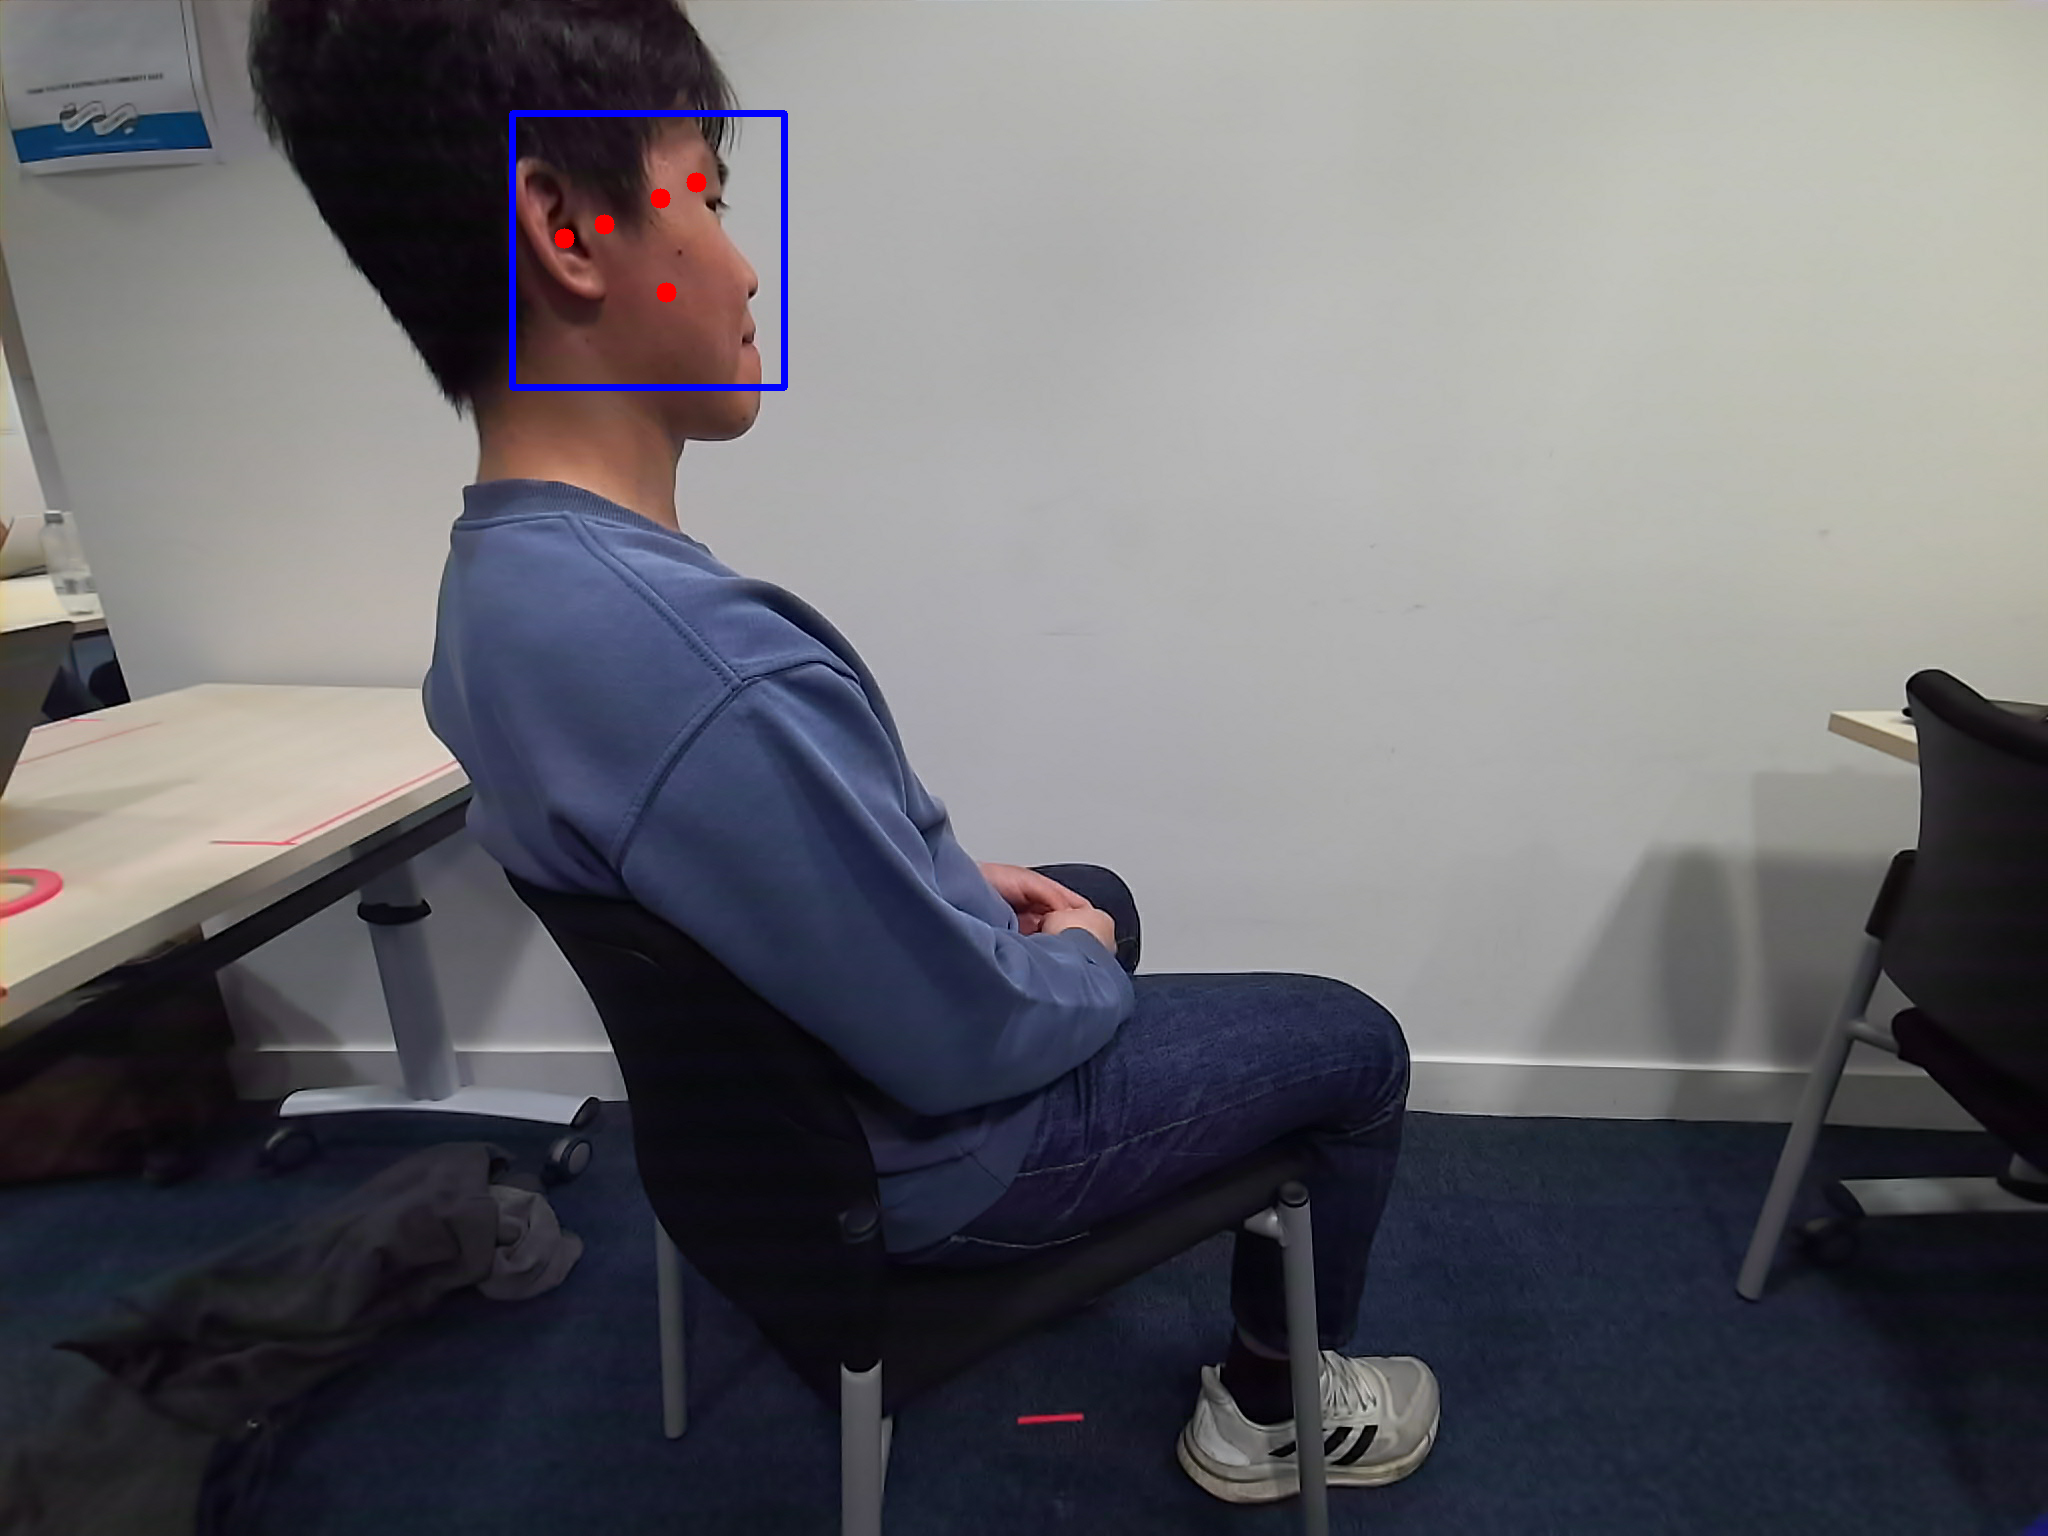
\includegraphics{./evaluation/figures/incorrectTrackedFace.png}
        }
    }
\end{invisBox}

As shown in Figure~\ref{fig:incorrect-head-track}, the face tracking model can still detect a face even when it is not visible, such as when detecting the side of the participant's head. The model tends to fail when only hair is visible. Testing on a bald participant could determine whether the system always detects a head regardless of rotation. While this might seem problematic, it is not, as the tracker and display are not visible to the user if their face is not visible. This also allows the system to approximate the position of the eyes, facilitating a smoother transition as the user turns their head back into view, minimizing the need for corrections and reducing noticeable adjustments for the user.

\subsubsection{Hand Tracking}

During the evaluation of our hand tracking model, we observed that it was significantly less reliable compared to our head tracking model, even when tested on the same images. Based on the metrics recorded during our user study, as illustrated in Fig~\ref{fig:failrate}, the hand tracking model failed for some users up to 10\% of the time, whereas the eye tracking model rarely experienced failures. This issue was particularly prominent when the model attempted to initially detect the hand. We found that the model was sensitive to specific conditions: it required a well-lit environment, a plain background, and the removal of extraneous objects from the scene. Users wearing t-shirts with intricate patterns experienced a notable decrease in tracking success. To address this, we provided a plain jumper for users to wear if we identified this as a potential problem. \\

We considered mitigating this issue by employing a segmentation model to separate the hand from the background before tracking. However, we did not have sufficient time to experiment with this solution, and we were concerned that it might significantly degrade the system's latency performance.

\begin{figureBox}[label={fig:failrate}, width=0.8\linewidth]{Failure rates during user study}
    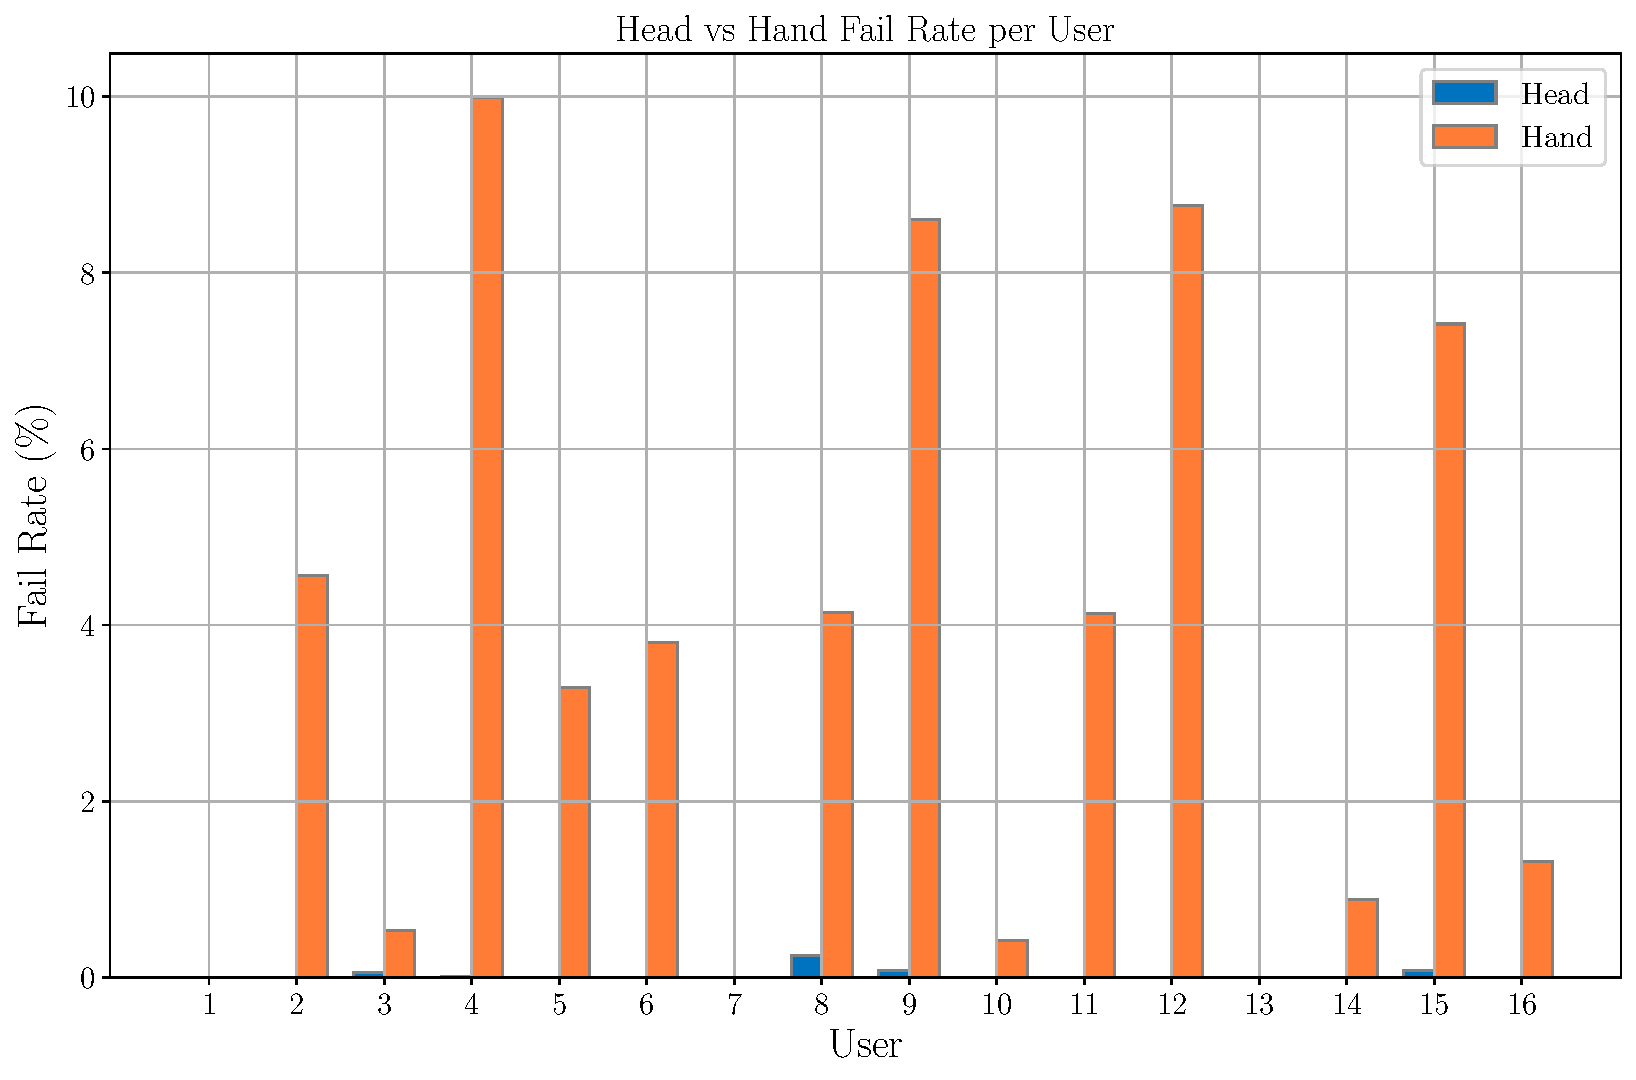
\includegraphics[width = 1.0\linewidth]{./evaluation/figures/failrate.pdf}
\end{figureBox}

A major challenge of using a depth sampling method is its inability to handle occlusion effectively. Although Mediapipe can predict the position of hand points even when they are not directly visible, our method struggles to sample their 3D positions accurately in such cases. This is problematic because the hand often occludes itself, as demonstrated in Fig~\ref{fig:occlusion}, where fingers are occluded by the palm, leading to erroneous depth sampling of the palm instead. Initially, we were concerned that this might also affect glasses wearers. However, we discovered that the depth sampling method, which uses infrared (IR) technology, was able to penetrate through glass.

\begin{figureBox}[label={fig:occlusion}, width=1.0\linewidth]{Occlusion in Sampling}
    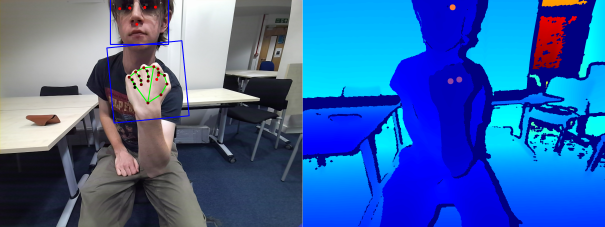
\includegraphics[width = 1.0\linewidth]{./evaluation/figures/occulusionsampling.png}
\end{figureBox}

There are methods to mitigate these issues, such as sampling from points that are not occluded and using the known depth of the hand to infer the depth of the occluded points. This is a complex problem, and we did not have sufficient time to develop a solution that was both accurate and fast. Additionally, we found that the relative depth values estimated by Mediapipe were not very accurate, complicating interaction. We believe that the most effective solution would be to switch to a point cloud-based tracking model \cite{sharp2015accurate}. Our solution was to switch to interaction using the middle and index fingers, the two fingers we found to be most reliable.

\subsection{Renderer}

In evaluating our rendering system, we focused primarily on the quality and accuracy of the images it produced.

\subsection[short]{Quality}

To evaluate the quality of our rendering system, we rendered a variety of complex 3D objects, including a chess set, a Minecraft house, and a protein structure. The images produced by our system were of high quality, as shown in Figures~\ref{fig:chess}, \ref{fig:erato}, \ref{fig:house}, and \ref{fig:8qbk}. The system was able to render these objects with high fidelity, accurately representing their 3D structure. The images were sharp and detailed, with precise lighting and shading. The system effectively rendered complex objects with numerous details, such as the protein structure, without any noticeable loss of quality or drop in frame rate. The images produced by our system were comparable to those produced by professional rendering software, demonstrating the high quality of our system.

\begin{invisBox}  
	\pictureBox[label={fig:chess}]{Chess Set \cite{noauthor_chessset_nodate}}{
	  \adjustbox{height=5cm, keepaspectratio}{
		\includegraphics{./evaluation/figures/renderer/chess_croped.png}
	  }
	}
	\hfill
	\pictureBox[label={fig:erato}]{Erato \cite{McGuire2017Data}}{
	\adjustbox{height=5cm, keepaspectratio}{
	  \includegraphics{./evaluation/figures/renderer/erato_2_cropped.png}
	  }
	}
	\\[0.3cm]
	\pictureBox[label={fig:house}]{Minecraft House \cite{McGuire2017Data}}{
	  \adjustbox{height=5cm, keepaspectratio}{
		\includegraphics{./evaluation/figures/renderer/house_2_cropped.png}
	  }
	}
	\hfill
	\pictureBox[label={fig:8qbk}]{Retron-Eco1 filament with ADP-ribosylated Effector \cite{bank_rcsb_nodate}}{
	\adjustbox{height=5cm, keepaspectratio}{
	  \includegraphics{./evaluation/figures/renderer/8qbk_cropped.png}
	  }
	}
\end{invisBox}

We successfully loaded and rendered a 6 million triangle model of Rungholt, a medieval city that was destroyed by a storm surge in the 14th century and recreated in Minecraft, as shown in Figure~\ref{fig:rungholt}. The model was rendered with no frame rate issues, demonstrating the system's ability to handle large and complex models with ease.

\begin{figureBox}[label={fig:rungholt}, width=1.0\linewidth]{Rungholt \cite{McGuire2017Data}}
	\includegraphics[width = 1.0\linewidth]{./evaluation/figures/renderer/rungholt_cropped.png}
\end{figureBox}

\subsubsection{Accuracy}

To evaluate the accuracy of our rendering system, we aimed to determine how well it could recreate a real object in a virtual environment. We chose a cube as our test object due to its simplicity and ease of measurement. A physical cube was constructed using Lego, and a corresponding virtual cube was created in our simulator, both with the exact dimensions of 13.5 cm x 13.5 cm x 12 cm, as illustrated in Figure~\ref{fig:real-vs-rendered}.

\begin{figureBox}[label={fig:real-vs-rendered}, width=1.0\linewidth]{A real and rendered cube}
	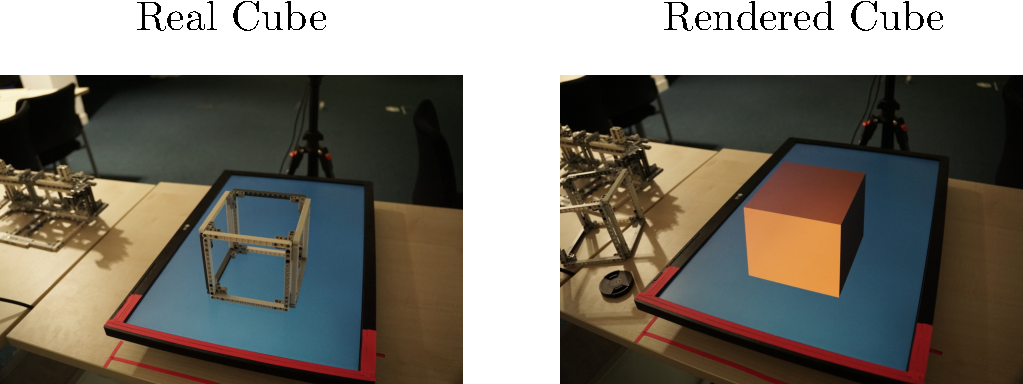
\includegraphics[width = 1.0\linewidth]{./evaluation/figures/real-vs-rendered.pdf}
\end{figureBox}

Due to the hollow nature of the physical cube, we were able to compare the two cubes effectively by superimposing them. We tested various perspectives and confirmed that the two cubes were indeed of the same size and shape, visually overlapping completely. Some example perspectives are presented in Figure~\ref{fig:super-imposed}. It is important to note that slight discrepancies in the images may occur, as the system was tracking the photographer's eye rather than the camera lens, which was positioned below and approximately 10 cm in front of the eye. Adjustments were made to account for this difference. This evaluation demonstrates that our rendering system is accurate and capable of recreating 3D objects from the real world with high precision.

\begin{figureBox}[label={fig:super-imposed}, width=1.0\linewidth]{Superimposed real and rendered cube}
	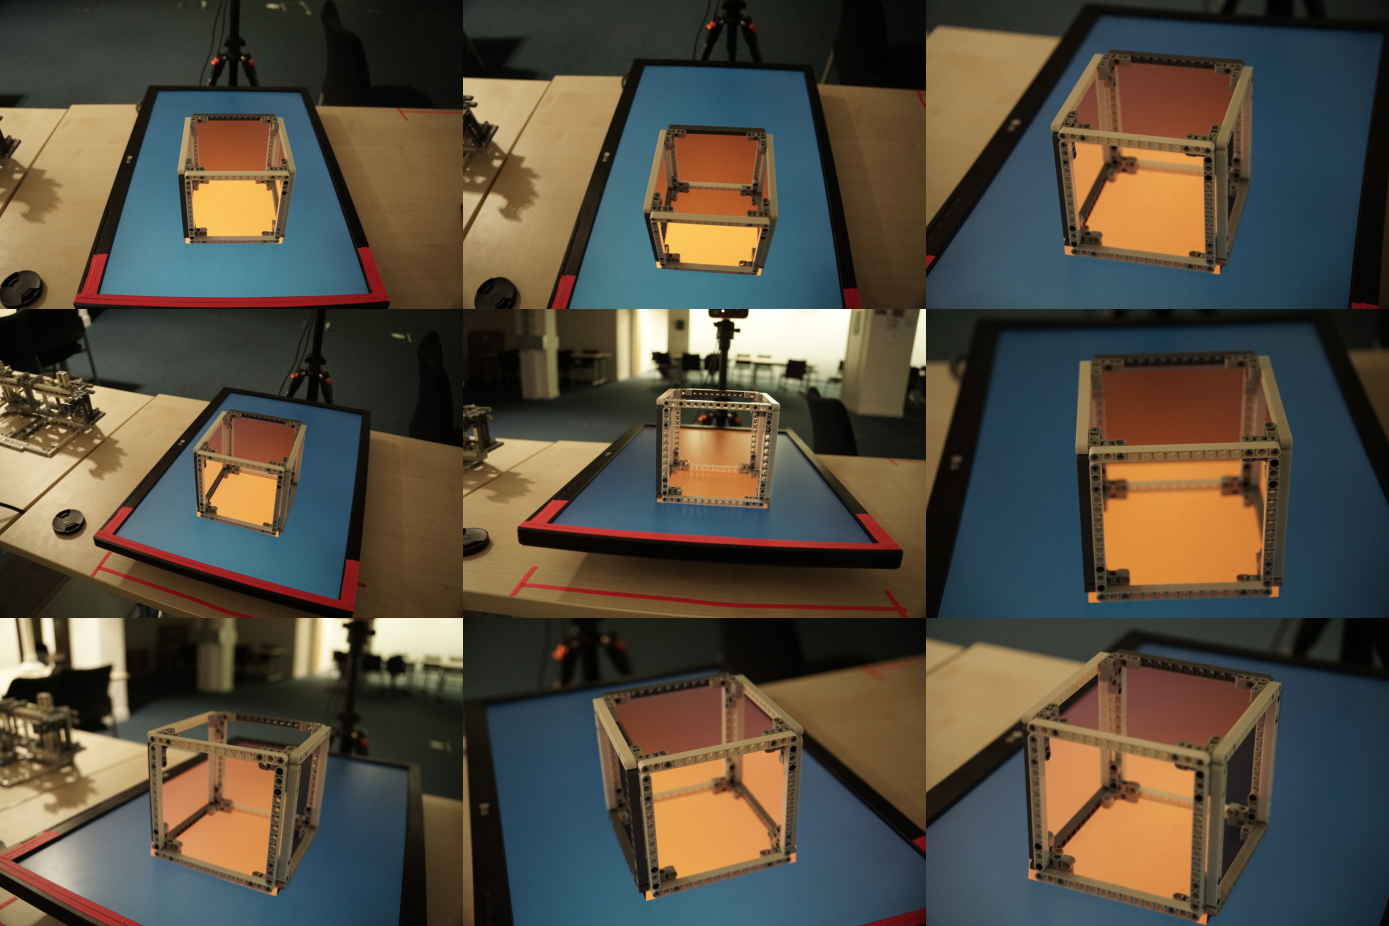
\includegraphics[width = 1.0\linewidth]{./evaluation/figures/super-imposed.pdf}
\end{figureBox}


\subsection{Portability}
One of the significant advantages of this system is its reproducibility and ease of deployment. It can be set up on a fresh Linux machine from scratch with a single command. The system was developed on a Linux machine (NixOS) using an Intel i5-9600K CPU and an NVIDIA GeForce RTX 2070 Super GPU. For testing purposes, the system was also run on a different Linux machine (NixOS) equipped with an Intel i7-4770K CPU and an NVIDIA GeForce GTX 1080 GPU, as depicted in Fig.~\ref{fig:other-machine}. Remarkably, the system executed flawlessly on the first attempt on this different hardware configuration.

\begin{figureBox}[label={fig:other-machine}, width=0.7\linewidth]{Running on a different machine}
	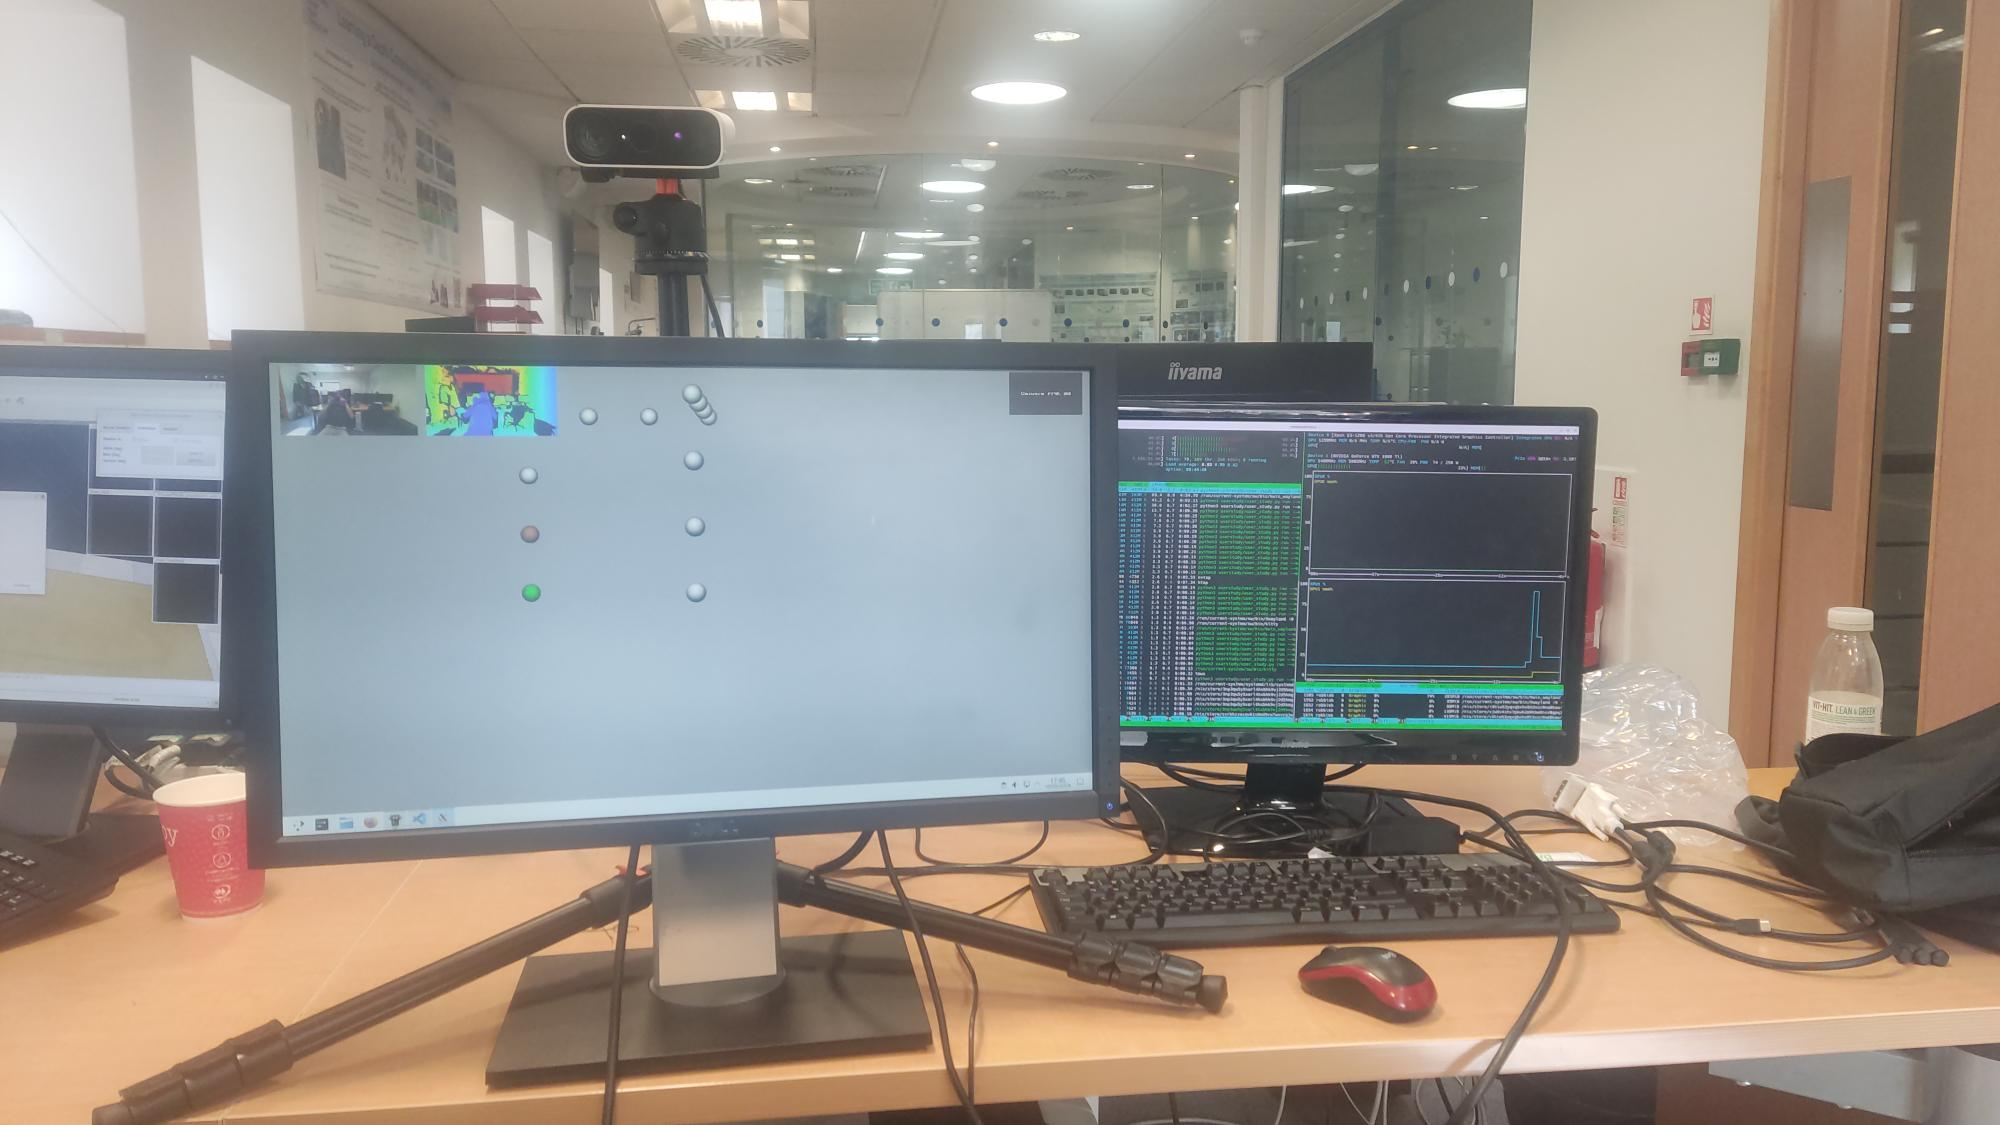
\includegraphics[width=1.0\linewidth]{./evaluation/figures/other-device.jpeg}
\end{figureBox}

We also tested the system on a Windows machine using Windows Subsystem for Linux 2 (WSL2). Although we successfully built the system, the OpenGL renderer did not function as expected. We did not have sufficient time to diagnose the issue thoroughly, but we suspect it is related to WSL GPU passthrough limitations. This issue is likely resolvable with additional troubleshooting. \\

Currently, the system only supports machines with Intel CPUs and NVIDIA GPUs. However, extending support to AMD CPUs and GPUs should be feasible with further development and fairly trivial modifications to the build system.

\subsection{Comparison to Other Systems}

As the field of volumetric displays is relatively new, there are few comparable systems available for direct comparison. However, we can compare our system to a few other devices that have been created. The most similar system to ours is the Multi-person Fish-Tank Virtual Reality Display \cite{10.1145/3281505.3281540} \cite{10.1145/169059.169066}, which uses a similar Kinect camera for tracking. \textcolor{red}{todo}

\begin{table}[h!]
	\centering
	\begin{tabular}{|>{\centering\arraybackslash}m{4cm}|>{\centering\arraybackslash}m{4cm}|>{\centering\arraybackslash}m{4cm}|>{\centering\arraybackslash}m{4cm}|}
	\hline
	\textbf{Attribute} & \textbf{Volumetric Simulator (Ours)} & \textbf{Fish-Tank Virtual
	Reality Display} \\
	\hline
	Attribute 1 & 0 & 0  \\
	\hline
	Attribute 2 & 0 & 0  \\
	\hline
	Attribute 3 & 0 & 0  \\
	\hline
	Attribute 4 & 0 & 0  \\
	\hline
	Attribute 5 & 0 & 0  \\
	\hline
	\end{tabular}
	\caption{Comparison of systems based on attributes}
	\label{table:comparison}
\end{table}

\textcolor{red}{TODO} 
\label{sect:eval-volsim}
\section{User Study}
\subsection{Introduction}
\begin{enumerate}
	\item The user study was conducted to evaluate the effectiveness of the system in improving the spatial reasoning skills of the participants.
\end{enumerate}

To validate the usefulness of our system we decided to conduct a Within-Subjects User Study. The user study was designed to show the capacity of the system for being used in research. The study was designed to test the effectiveness of users using volumetric displays under different conditions.

\subsection{Experimental Variables}
\begin{enumerate}
	\item Independent Variables:
	\begin{enumerate}
		\item 3D Perspective (On/Off)
		\item Interaction Offset (On/Off)
		\item So 4 conditions
	\end{enumerate}
	\item Dependent Variables:
	\begin{enumerate}
		\item Time taken to complete task
		\item Number of subtasks completed
		\item Eye and hand positions
	\end{enumerate}
	\item Control Variables:
	\begin{enumerate}
		\item The five tasks are the same in each condition.
		\item Position of participant
		\item Position of the tracking camera
		\item Position of the zone of interaction
		\item Size of the display. 
	\end{enumerate}
	\item Confounding Variables:
	\begin{enumerate}
		\item The participants may have different levels of experience with VR/Volumetric.
		\item Left-handed vs right-handed might make a difference for the tasks.
		\item Wearing glasses might make a difference for head tracking.
	\end{enumerate}
	\item 
\end{enumerate}

For this study we wanted to evaluate the difference in performance of participants in interacting with volumetric screens with their hands. 

Our two independent variables were: 
\begin{itemize}[itemsep=-0.25em]
	\item \textbf{3D Perspective}: (On/Off). This controls if the system is able to use the eye tracking system to create the illusion of a 3D volumetric display as can be seen in Fig~\todo.
	\item \textbf{Interaction Offset}: (On/Off). This controls if display is directly in front of the participant or if it is offset by a fixed amount as can be seen in Fig~\todo.
\end{itemize}
Giving us a total of 4 conditions to test.


The first condition we wanted to test was if there was any noticeable drop in performance when using the system in 2D (i.e with eye tracking disabled but still using hand tracking). The second condition was if there was a performance difference if participants "teleoperated" (controlled it with a fixed offset) the simulator vs using their hands directly. Combining these two conditions gives us the four conditions we tested as can be seen in Fig~\ref{fig:study-conditions}. 

\subsection{Tasks}
\begin{enumerate}
	\item Trace out points like a buzzwire game. 
	\item Draw Diagram of how the task works
	\item Draw Isometric view of the tasks
	\item Tasks are designed to be annoying if not in 3D.
	\item Timeout of 1 minute.
\end{enumerate}

In each of the 4 conditions the participant must complete the same 5 tasks. The tasks are designed to be simple but more difficult to complete if not in 3D. To complete a task a participant must trace the path between the points with their index and middle finger in the order the simulator presents to them. A green point is completed and an orange point represents the next point ot be completed as can be seen in Fig~\todo. \\ 

The participants have a timeout of 1 minute to complete the task. If they do not complete the task in the time limit, the task is marked as incomplete. The time each point is completed is recorded as well as the position of the hand and eye throughout the minute. The 5 different tasks are shown in Fig~\todo.

\subsection{Study Implementation}
\begin{enumerate}
	\item We run the study from a python based CLI (Click).
	\item We compile the simulator as a shared library and call it from the python CLI using a C-FFI.
	\item We receive the results and logs from python in json format and store them in a mongoDB database.
	\item This data is then used to generate the results.
\end{enumerate}

\subsection{Participants}
\begin{enumerate}
	\item We record age, gender, if they are left or right handed, and if they have any experience with VR, and if they wear glasses.
	\item The participants were given a random order of the four conditions.
	\item They complete the 5 tasks in each
	\item Fill out survey about each condition.
	\item Fill out survey about the system as a whole at the end.
	\item Ran the study in Huxley building.
\end{enumerate}

\subsection{Study Results}
\begin{enumerate}
	\item Use ANOVA test?
	\item ????
\end{enumerate}

\label{sect:eval-userstudy}

%%%%%%%%%%%%%%%%%%%%%%%%%%%%%%%%%%%%
\chapter{Future Work, Conclusions and Contributions}
\section{Future Work}

We have identified several areas for future work that could enhance the capabilities and usability of our volumetric display simulator and further explore the potential of volumetric displays in interactive 3D applications.

\subsection{Anaglyph 3D}
Anaglyph 3D \cite{Dhaou2019} is a technique for displaying 3D images using colour-filtered glasses, typically employing red and green filters. Unlike polarized 3D \cite{article-3D}, it does not require additional complex hardware. Currently, the 3D effect necessitates closing one eye. Integrating 3D support into the system could enhance the immersive experience by eliminating this limitation.

\subsection{Multi-User Support}
Another potential area for future exploration is multi-user support. Our current tracking system is limited to a single user. Extending it to support multiple users would be a logical progression and relatively straightforward. By utilizing colour filter glasses or shutter glasses, it is feasible to render different perspectives to multiple users simultaneously, as suggested in the study "Two Kinds of Novel Multi-user Immersive Display Systems" \cite{Two-Kinds}.

\subsection{Real-Time Light Detection}
Adding an additional camera with a fisheye lens to generate a real-time light map could be a valuable enhancement. This feature would enable the virtual scene to be illuminated by real-world lighting conditions. It would be insightful to investigate whether this addition impacts performance in any significant way, especially concerning the tasks evaluated in our user study.

\subsection{Generalize CPU/GPU Camera Compatibility}
The current project is compatible only with Nvidia GPUs. Expanding compatibility to include AMD GPUs, Intel GPUs, and even CPU-only environments (with expected slower performance) would be beneficial. Furthermore, supporting different depth cameras beyond the Kinect, such as Intel RealSense Depth Cameras \cite{keselman2017intel}, is crucial, particularly since the Kinect has been discontinued by Microsoft. Achieving this will require substantial code generalization. Switching cameras to a lower latency system would also be beneficial.

\subsection{Switch Hand Tracking Model}
The hand tracking component of the project is notably the weakest aspect. Transitioning to a more robust hand tracking model is highly recommended. Specifically, adopting a model that utilises depth images rather than RGB images could significantly improve performance. This would likely be a major undertaking, as off-the-shelf models for this purpose are scarce. Implementing the approach described in the paper "Accurate, Robust, and Flexible Real-Time Hand Tracking" \cite{sharp2015accurate} appears promising.

\subsection{Further User Study}
As indicated in the evaluation section, while the user study provided conclusive results, further investigation is warranted. We are interested in exploring various offset positions to examine the drop-off rate in greater detail. Additionally, adjusting the position of the interaction zone, as opposed to the display position, could yield valuable insights.

\subsection{Porting to Windows and Mac}
Although we have demonstrated that the project can be built with a single command on Linux, extending support to Windows (including WSL) and Mac would be advantageous. We have successfully compiled the project on Windows, but further investigation is required to address WSL-specific issues. We have yet to attempt building it on Mac. This is expected to be more challenging, as porting all GPU-accelerated functionality to Apple Metal \cite{noauthor_httpsdeveloperapplecommetalmetal-shading-language-specificationpdf_nodate} may pose significant difficulties, despite Nix's native compatibility with Mac.

\section{Conclusions}

The development and evaluation of our Volumetric Display Simulator underscore its potential as a versatile tool for future research in volumetric display technologies. By integrating cost-effective components and reproducible software environments, we have created a system that is both accessible and straightforward, encouraging wider adoption and further development by other researchers. \\

Our user study demonstrated that the use of head tracking and direct hand interaction significantly enhances task performance in a 3D environment, highlighting the importance of natural interaction modes for effective use of volumetric displays. The findings suggest promising avenues for future research, including the exploration of positional offsets and interaction zone dynamics, which could lead to significant improvements in the usability and functionality of volumetric displays.
\label{sect:conclusions}

%%%%%%%%%%%%%%%%%%%%%%%%%%%%%%%%%%%%
\printbibliography

\appendix
\chapter{Final Package}
\label{app:final-package}
\section{VolumetricSim Package}
The result of building our simulator is a shared library named \texttt{libvolsim.so} shown in Listing~\ref{list:libvolsim}.
\codeBoxFile[label = {list:libvolsim}]{shell}{./implementation/code/libvolsim.sh}{Terminal}
\chapter{Survey Forms}
\label{app:survey}
\section{Form A: Overall Digital Survey Form}
This form is the primary survey that was given to participants in the user study. It was used to collect data on the participants' demographics, their experience with technology, and their opinions on the volumetric display system.


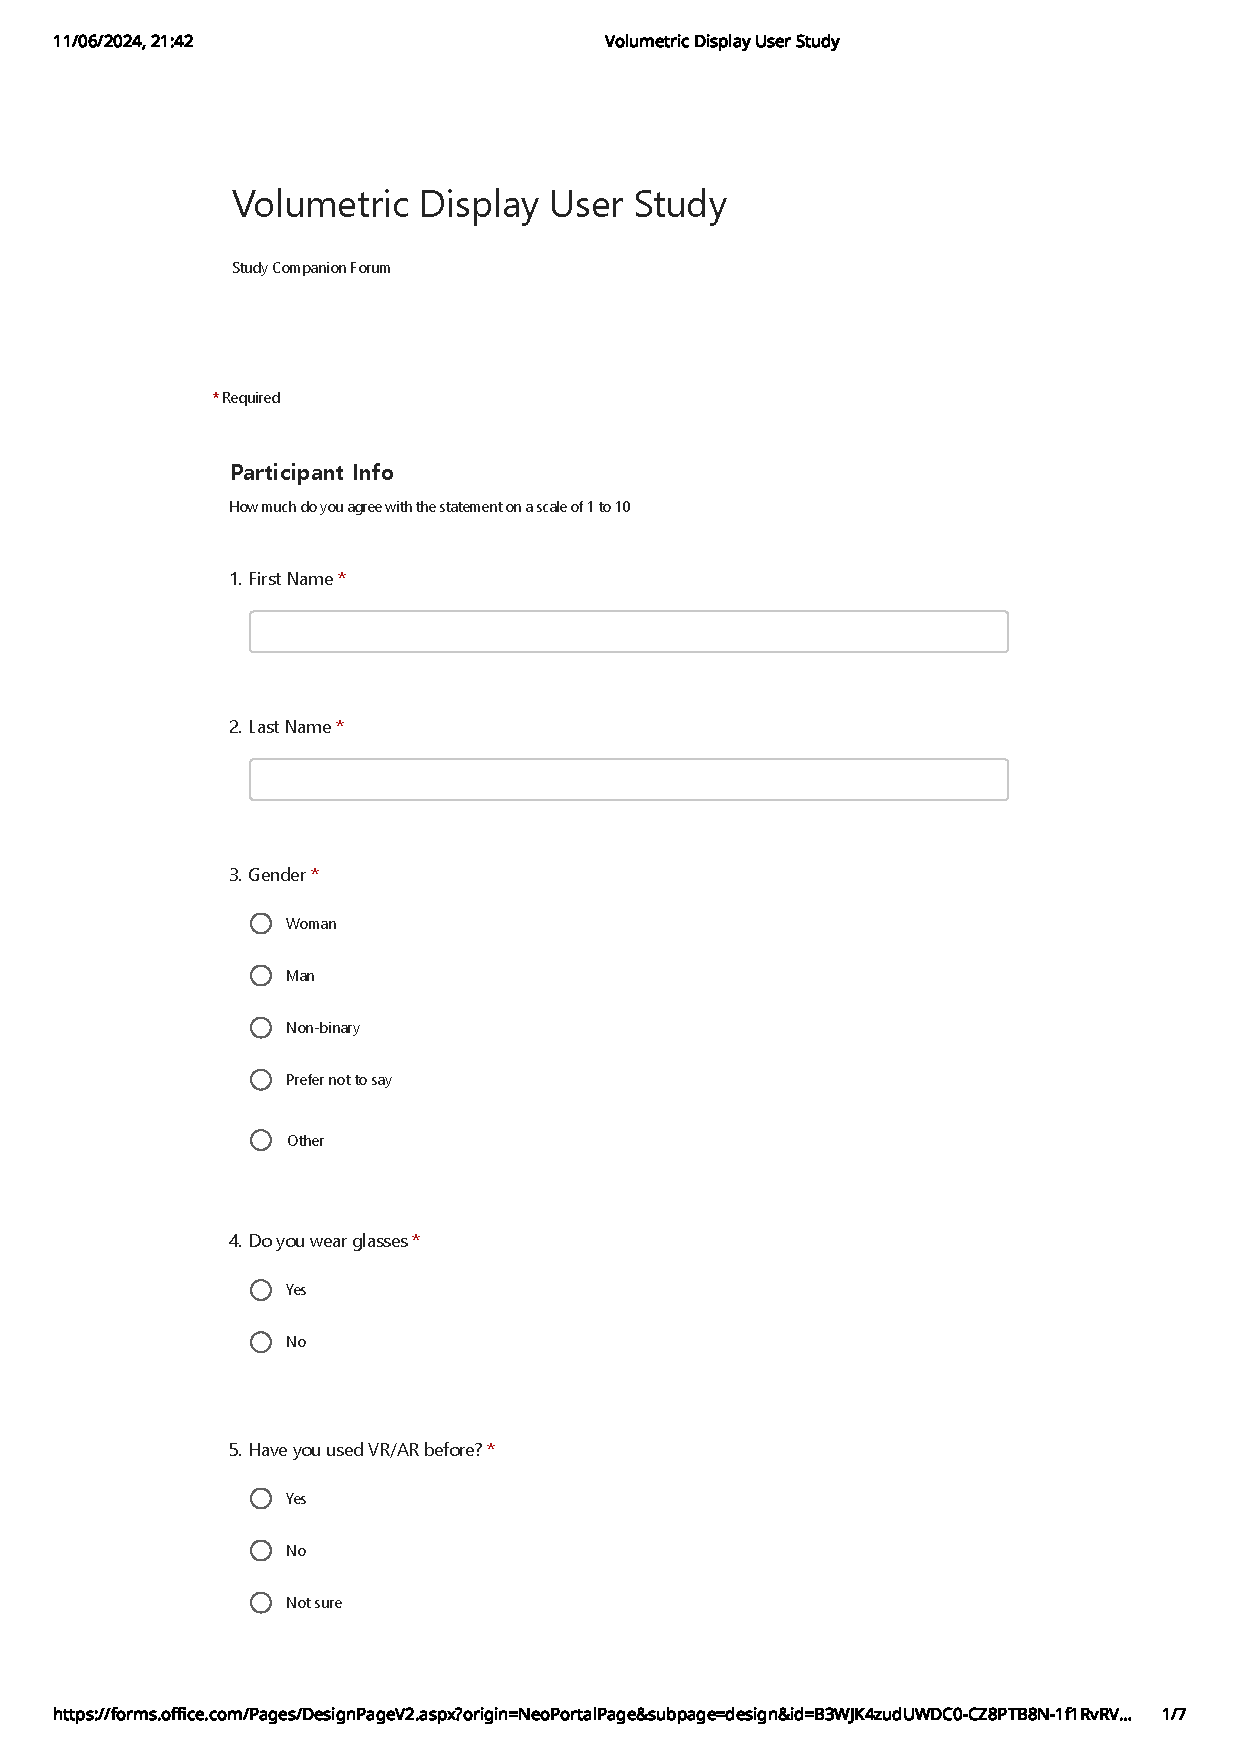
\includepdf[pages=-]{./appendix/files/Volumetric Display User Study.pdf}
\section{Form B: Inter-Condition Survey Form}
This was the phyiscal survey that was given to participants in the user study. It was used to collect data on the participants' opinions between the different conditions of the volumetric display system. The results were copied into a digital form. 

\includepdf[pages=-]{./appendix/files/Document For User Study.pdf}
\chapter{Extended User Study Results}
\label{app:results}
\section{Comprehensive Results}
Presented below are the detailed graphs and results from our user study, organized on a task-by-task basis. The graphs are divided into five sections, each corresponding to a specific task. The first two graphs are similar to those found in Evaluation~\ref{sect:eval-userstudy}, but are applied exclusively to this task. The subsequent four graphs display the fully plotted 3D paths of users under each condition, with each segment represented in a distinct colour.

\newpage
\includegraphics[scale=0.8]{./appendix/files/graphs-1.png}
\newpage
\includegraphics[scale=0.8]{./appendix/files/graphs-2.png}
\newpage
\includegraphics[scale=0.8]{./appendix/files/graphs-3.png}
\newpage
\includegraphics[scale=0.8]{./appendix/files/graphs-4.png}
\newpage
\includegraphics[scale=0.8]{./appendix/files/graphs-5.png}

\end{document}